\documentclass[fontsize=11pt, paper=a4, twoside=true, BCOR=5mm, DIV=10]{scrbook}

% -------------------------------------------------------------------
% PAQUETES Y OPCIONES
% -------------------------------------------------------------------
\RequirePackage[utf8]{inputenc} 
\RequirePackage[english, spanish, es-nodecimaldot, es-noindentfirst, es-tabla]{babel}

\usepackage{listings}
\usepackage{dcolumn}
\usepackage{enumitem}
\usepackage[chapter]{algorithm}
\usepackage{algpseudocode}
\RequirePackage{verbatim}
%\RequirePackage[Glenn]{fncychap}
\usepackage{fancyhdr}
\usepackage{graphicx}
%\usepackage{doxygen/doxygen}
\usepackage{pdfpages}
\usepackage{url}
\usepackage{colortbl,longtable}
\usepackage[stable]{footmisc}
\usepackage{index}


\newcolumntype{.}{D{.}{\esperiod}{-1}}
\makeatletter
\addto\shorthandsspanish{\let\esperiod\es@period@code}
\makeatother

\DeclareUnicodeCharacter{200B}{}

\usepackage[pdfborder={000}]{hyperref} %referencia

% -------------------------------------------------------------------
% INFORMACIÓN DEL TFG Y EL AUTOR
% -------------------------------------------------------------------
\newcommand{\myTitle}{Título del proyecto\xspace}
\newcommand{\myDegree}{Grado en Ingeniería informática}
\newcommand{\myName}{Cristhian Moya Mota (alumno)\xspace}
\newcommand{\myProf}{Diego Jesús García Gil (tutor1)\xspace}
\newcommand{\myOtherProf}{Julián Luengo Martín (tutor2)\xspace}
%\newcommand{\mySupervisor}{Put name here\xspace}
\newcommand{\myFaculty}{Escuela Técnica Superior de Ingenierías Informática y de
Telecomunicación\xspace}
\newcommand{\myFacultyShort}{E.T.S. de Ingenierías Informática y de
Telecomunicación\xspace}
\newcommand{\myDepartment}{Departamento de ...\xspace}
\newcommand{\myUni}{\protect{Universidad de Granada}\xspace}
\newcommand{\myLocation}{Granada\xspace}
\newcommand{\myTime}{\today\xspace}
\newcommand{\myVersion}{Version 0.1\xspace}


% -------------------------------------------------------------------
% ESTILOS DE LA CLASE KOMA
% -------------------------------------------------------------------
% Selecciona el tipo de fuente para los títulos (capítulo, sección, subsección) del documento.
\setkomafont{disposition}{\sffamily\bfseries}

% Cambia el ancho de la cita. Al inicio de un capítulo podemos usar el comando \dictum[autor]{cita} para añadir una cita famosa de un autor.
\renewcommand{\dictumwidth}{0.45\textwidth} 

\recalctypearea % Necesario tras definir la tipografía a usar.

\hypersetup{
	    pdfauthor = {\myName (email (en) ugr (punto) es)},
		% hidelinks,            % Enlaces sin color ni borde. El borde no se imprime
		linkbordercolor=0.8 0 0,
		citebordercolor=0 0.8 0,
		citebordercolor=0 0.8 0,
		colorlinks = true,            % Color en texto de los enlaces. Comentar esta línea o cambiar `true` por `false` para imprimir el documento.
		linkcolor = [rgb]{0.5, 0, 0}, % Color de los enlaces internos
		urlcolor = [rgb]{0, 0, 0.5},  % Color de los hipervínculos
		citecolor = [rgb]{0, 0.5, 0}, % Color de las referencias bibliográficas
		pdfsubject={Trabajo de fin de Grado},%
		pdfkeywords = {palabra_clave1, palabra_clave2, palabra_clave3, ...},
		pdfcreator={pdfLaTeX}%
	}


% Normal font: 			URW Palladio typeface. 
% Sans-serif font: 	Gill Sans (paquete cabin)
% Monospace font: 	Inconsolata
\RequirePackage[T1]{fontenc}
\RequirePackage[sc, osf]{mathpazo} \linespread{1.05}         
\IfFileExists{cabin.sty}{
	\RequirePackage[scaled=.95,type1]{cabin} 
} %else
{
	% Si cabin da ERROR usar el siguiente comando en su lugar
	\renewcommand{\sfdefault}{iwona} 
}

%\hyphenation{}


%\makeindex
%\usepackage[style=long, cols=2,border=plain,toc=true,number=none]{glossary}
% \makeglossary

% Definición de comandos que me son tiles:
%\renewcommand{\indexname}{Índice alfabético}
%\renewcommand{\glossaryname}{Glosario}

\pagestyle{fancy}
\fancyhf{}
\fancyhead[LO]{\leftmark}
\fancyhead[RE]{\rightmark}
\fancyhead[RO,LE]{\textbf{\thepage}}
\renewcommand{\chaptermark}[1]{\markboth{\textbf{#1}}{}}
\renewcommand{\sectionmark}[1]{\markright{\textbf{\thesection. #1}}}

\setlength{\headheight}{1.5\headheight}

\newcommand{\HRule}{\rule{\linewidth}{0.5mm}}
%Definimos los tipos teorema, ejemplo y definición podremos usar estos tipos
%simplemente poniendo \begin{teorema} \end{teorema} ...
%\newtheorem{teorema}{Teorema}[chapter]
%\newtheorem{ejemplo}{Ejemplo}[chapter]
%\newtheorem{definicion}{Definición}[chapter]

\definecolor{gray97}{gray}{.97}
\definecolor{gray75}{gray}{.75}
\definecolor{gray45}{gray}{.45}
\definecolor{gray30}{gray}{.94}

\lstset{ frame=Ltb,
     framerule=0.5pt,
     aboveskip=0.5cm,
     framextopmargin=3pt,
     framexbottommargin=3pt,
     framexleftmargin=0.1cm,
     framesep=0pt,
     rulesep=.4pt,
     backgroundcolor=\color{gray97},
     rulesepcolor=\color{black},
     %
     stringstyle=\ttfamily,
     showstringspaces = false,
     basicstyle=\scriptsize\ttfamily,
     commentstyle=\color{gray45},
     keywordstyle=\bfseries,
     %
     numbers=left,
     numbersep=6pt,
     numberstyle=\tiny,
     numberfirstline = false,
     breaklines=true,
   }
 
% minimizar fragmentado de listados
\lstnewenvironment{listing}[1][]
   {\lstset{#1}\pagebreak[0]}{\pagebreak[0]}

\lstdefinestyle{CodigoC}
   {
	basicstyle=\scriptsize,
	frame=single,
	language=C,
	numbers=left
   }
\lstdefinestyle{CodigoC++}
   {
	basicstyle=\small,
	frame=single,
	backgroundcolor=\color{gray30},
	language=C++,
	numbers=left
   }

 
\lstdefinestyle{Consola}
   {basicstyle=\scriptsize\bf\ttfamily,
    backgroundcolor=\color{gray30},
    frame=single,
    numbers=none
   }


\newcommand{\bigrule}{\titlerule[0.5mm]}


%Para conseguir que en las páginas en blanco no ponga cabecerass
\makeatletter
\def\clearpage{%
  \ifvmode
    \ifnum \@dbltopnum =\m@ne
      \ifdim \pagetotal <\topskip
        \hbox{}
      \fi
    \fi
  \fi
  \newpage
  \thispagestyle{empty}
  \write\m@ne{}
  \vbox{}
  \penalty -\@Mi
}
\makeatother

% -------------------------------------------------------------------
% DESARROLLO DE LOS CAPÍTULOS DEL TRABAJO
% -------------------------------------------------------------------

\begin{document}
	% Plantilla portada UGR
	\begin{titlepage}
 
\newlength{\centeroffset}
\setlength{\centeroffset}{-0.5\oddsidemargin}
\addtolength{\centeroffset}{0.5\evensidemargin}
\thispagestyle{empty}

\noindent\hspace*{\centeroffset}\begin{minipage}{\textwidth}

\centering

\includegraphics[width=0.9\textwidth]{imagenes/logo_ugr.jpg}\\[1.4cm]

\textsc{ \Large TRABAJO FIN DE GRADO\\[0.2cm]}
\textsc{ INGENIERÍA INFORMÁTICA}\\[1cm]
% Upper part of the page
% 
% Title
{\Huge\bfseries Aplicación móvil para la prognosis y detección del cáncer de piel usando Deep Learning\\
}
\noindent\rule[-1ex]{\textwidth}{3pt}\\[3.5ex]
%{\large\bfseries Subtitulo del Proyecto}
\end{minipage}

\vspace{1cm}
\noindent\hspace*{\centeroffset}\begin{minipage}{\textwidth}
\centering

\textbf{Autor}\\ {Cristhian Moya Mota (alumno)}\\[2ex]
\textbf{Directores}\\
Diego Jesús García Gil\\
Julián Luengo Martín\\
\vspace{2cm}

\includegraphics[width=0.3\textwidth]{imagenes/etsiit_logo.png}\\[0.1cm]
\textsc{Escuela Técnica Superior de Ingenierías Informática y de Telecomunicación}\\
\textsc{---}\\
Granada, \today
\end{minipage}
%\addtolength{\textwidth}{\centeroffset}
%\vspace{\stretch{2}}
\end{titlepage}



	
	% Plantilla prefacio UGR
	\chapter*{}
%\thispagestyle{empty}
%\cleardoublepage

%\thispagestyle{empty}

\begin{titlepage}
 
 
\setlength{\centeroffset}{-0.5\oddsidemargin}
\addtolength{\centeroffset}{0.5\evensidemargin}
\thispagestyle{empty}

\noindent\hspace*{\centeroffset}\begin{minipage}{\textwidth}

\centering
%
\includegraphics[width=0.9\textwidth]{imagenes/logo_ugr.jpg}\\[1.4cm]

%\textsc{ \Large PROYECTO FIN DE CARRERA\\[0.2cm]}
%\textsc{ INGENIERÍA EN INFORMÁTICA}\\[1cm]
% Upper part of the page
% 

 \vspace{3.3cm}

%si el proyecto tiene logo poner aquí

\includegraphics{imagenes/logo.png} 
 \vspace{0.5cm}

% Title

{\Huge\bfseries Aplicación móvil para la prognosis y detección del cáncer de piel usando Deep Learning\\
}
\noindent\rule[-1ex]{\textwidth}{3pt}\\[3.5ex]
%{\large\bfseries Subtítulo del proyecto.\\[4cm]}
\end{minipage}

\vspace{2.5cm}
\noindent\hspace*{\centeroffset}\begin{minipage}{\textwidth}
\centering

\textbf{Autor}\\ {Cristhian Moya Mota}\\[2.5ex]
\textbf{Directores}\\
{Nombre Apellido1 Apellido2 (tutor1)\\
Nombre Apellido1 Apellido2 (tutor2)}\\[2cm]
%
\includegraphics[width=0.15\textwidth]{imagenes/tstc.png}\\[0.1cm]
%\textsc{Departamento de Teoría de la Señal, Telemática y Comunicaciones}\\
%\textsc{---}\\
%Granada, mes de 201
\end{minipage}
%\addtolength{\textwidth}{\centeroffset}
\vspace{\stretch{2}}

 
\end{titlepage}






\cleardoublepage
\thispagestyle{empty}

\begin{center}
{\large\bfseries Aplicación móvil para la prognosis y detección del cáncer de piel usando deep learning}\\
\end{center}
\begin{center}
Cristhian Moya Mota\\
\end{center}

%\vspace{0.7cm}
\noindent{\textbf{Palabras clave}: cáncer de piel, deep learning, prognosis, diagnóstico, preprocesado, cuantización, aplicación Android.}\\

\vspace{0.7cm}
\noindent{\textbf{Resumen}}\\

El cáncer es una de las enfermedades que más muertes causan al año en todo el mundo. Su tendencia, en aumento, refleja la importancia de una correcta detección y diagnóstico de esta enfermedad a través de los médicos especialistas. Sin embargo, su elevado coste en algunos países, y la gran incidencia mostrada cada año dificulta el acceso a los medios adecuados para una parte considerable de la población, sobre todo, aquella con menos recursos. Uno de los más frecuentes, el cáncer de piel, suma a este problema la dificultad de diagnóstico, compleja incluso para los dermatólogos por su similitud con los lunares comunes.

La detección temprana de los tumores cutáneos, sobre todo de los de tipo melanoma, es clave para aumentar la esperanza de vida de sus pacientes. Para hacer más accesible el diagnóstico, se propone el uso de modelos de deep learning, cuyo modelo resultante tras el aprendizaje sea capaz de ejecutarse en un teléfono móvil, teniendo en cuenta las restricciones de potencia asociadas.

Se emplean, para lograrlo, los conjuntos de datos más citados y conocidos del estado del arte, mediante los cuales se procede a la creación de un conjunto combinado variado y suficientemente extenso como para diagnosticar no solo si se trata de una lesión benigna o maligna, si no también para especificar la enfermedad concreta a la que el paciente se enfrenta. Por tanto, convierte el proceso de tratamiento de los datos en un aspecto clave a tener en cuenta, que comprende la selección, el recortado y el reetiquetado manual de los datos para lograr la estandarización de los mismos y obtener un conjunto apto para el proceso de aprendizaje, tras aplicar un aumento de resolución mediante redes generativas adversarias (GANs)~\cite{goodfellow2014generative}.

Para esta tarea, se tienen en cuenta las restricciones de potencia impuestas por la arquitectura ARM de los smartphones, usando para ello el proceso de cuantización de modelos. Tras un análisis de los modelos habitualmente aplicados, se demuestra que la simplificación mediante cuantización consigue mejores resultados que los modelos pensados inicialmente para ser ejecutados en dispositivos de baja potencia. Además, se emplea un enfoque novedoso por el cual, en lugar de construirse un único modelo, se construyen 3 modelos organizados a dos niveles para reducir al mínimo las pérdidas ocasionadas por la cuantización, siendo uno específico para distinguir en un primer nivel, si se trata de una enfermedad maligna o benigna, y posteriormente, emplear uno de los dos modelos especializados en cada una de las variantes.

Esta arquitectura consigue unos resultados cercanos a un 83\% de acierto en clasificación binaria, y un 82\%  y 45\% en enfermedades malignas y benignas, respectivamente, por lo que ofrece resultados razonables teniendo en cuenta la ganancia en velocidad obtenida tras realizar el proceso de cuantización, superior a 1,5 en los 3 casos. Además, todo ello se consigue con apenas un 1\% de pérdida respecto al modelo base, ResNet50~\cite{he2015deep}.

Por último, para poner en práctica el modelo entrenado, se ha desarrollado una aplicación Android que ofrece al usuario la capacidad de tomarse una fotografía de la lesión que desee diagnosticar, y obtener el resultado en un tiempo inferior a un segundo, sin necesidad de conectarse a servidores externos, y con la posibilidad de revisar los casos previamente diagnosticados y su evolución mediante un historial. 

\cleardoublepage
\thispagestyle{empty}


\begin{center}
{\large\bfseries Aplicación móvil para la prognosis y detección del cáncer de piel usando deep learning}\\
\end{center}
\begin{center}
Cristhian Moya Mota\\
\end{center}

%\vspace{0.7cm}
\noindent{\textbf{Keywords}: skin cancer, deep learning, prognosis, preprocessing, quantization,  Android app.}\\

\vspace{0.7cm}
\noindent{\textbf{Abstract}}\\

Cancer is one of the diseases that causes the most deaths each year worldwide. Recent studies say each year there will be more cases than previous. This reflects the importance of preventive detection and diagnosis by specialists . However, preventive medicine has a high cost in some countries. The high incidence shown each year make access to specialists a difficult task for a considerable part of the population, especially those with fewer resources. Skin cancer is one of the most frequent cancers in the world, and its similarity to other skin conditions like benign moles make the problem even harder for specialists.

Preventive medicine is the way to minimize the mortality of some skin cancers, like melanoma, which is the worst posible condition. In order to make prognosis an easier task, we propose the use of deep learning models, with the resulting model after learning being capable of running on a mobile phone, taking into account CPU power restrictions.

To achieve it, this project uses the most used and cited datasets in the state of art. With them, we made a big an exhaustive dataset which combines images to detect if a mole is benign or malign. But, we also have enough information to predict the type of benign or malign disease we have. Therefore, it turns the data processing process into a key aspect to consider, which includes data selection, cropping, and manual re-labeling to achieve standardization, and obtain a dataset suitable for the learning process, including the use of GANs (Generative Adversarial Netwoks)~\cite{goodfellow2014generative}.

To solve this problem, we take into account the performance and powers restrictions of the ARM architecture by utilizing quantization as a way to simplify models. After doing an analysis between the most common convolutional models, it is demonstrated that simplification through quantization achieves better results than models initially designed to run on low-power devices.  We also replaced the common technique of doing an unique model with a two level architecture instead, where we have 3 different models: the first one, to separate between benign and malignant moles, and the other two to prognosticate the specific type of disease it has. With this novel technique, we minimize the precision loss caused by quantization.

This architecture achieves results close to 83\% accuracy in binary classification. For specific diseases, achieves around 82\% and 45\% of accuracy for malignant and benign diseases, respectively. The speed gain achieved after quantization process is greater than 1.5 in all three cases. Furthermore, all of this is accomplished with just less than 1\% loss compared to the base model, ResNet50~\cite{he2015deep}.

In order to show the trained models, we developed an Android. It offers the user the ability to take a photograph of the lesion he/she want to diagnose and obtain the results within 1 second of delay, all of this without needing an external server. Furthermore, it provides the ability to save previously diagnosed cases to check their evolution through time.


\chapter*{}
\thispagestyle{empty}

\noindent\rule[-1ex]{\textwidth}{2pt}\\[4.5ex]

Yo, \textbf{Cristhian Moya Mota}, alumno de la titulación Grado en Ingeniería informática de la \textbf{Escuela Técnica Superior
de Ingenierías Informática y de Telecomunicación de la Universidad de Granada}, con DNI 20596451C, autorizo la
ubicación de la siguiente copia de mi Trabajo Fin de Grado en la biblioteca del centro para que pueda ser
consultada por las personas que lo deseen.

\vspace{6cm}

\noindent Fdo: Cristhian Moya Mota

\vspace{2cm}

\begin{flushright}
Granada a 24 de junio de 2024.
\end{flushright}


\chapter*{}
\thispagestyle{empty}

\noindent\rule[-1ex]{\textwidth}{2pt}\\[4.5ex]

D. \textbf{Diego Jesús García Gil}, Profesor del Departamento de Lenguajes y Sistemas Informáticos de la Universidad de Granada.

\vspace{0.5cm}

D. \textbf{Julián Luengo Martín}, Profesor del Departamento de Ciencias de la Computación e Inteligencia Artificial
 de la Universidad de Granada.


\vspace{0.5cm}

\textbf{Informan:}

\vspace{0.5cm}

Que el presente trabajo, titulado \textit{\textbf{Aplicación móvil para la prognosis y detección del cáncer de piel usando deep learning}},
ha sido realizado bajo su supervisión por \textbf{Cristhian Moya Mota}, y autorizamos la defensa de dicho trabajo ante el tribunal
que corresponda.

\vspace{0.5cm}

Y para que conste, expiden y firman el presente informe en Granada a 24 de junio de 2024.

\vspace{1cm}

\textbf{Los directores:}

\vspace{5cm}

\noindent \textbf{Diego Jesús García Gil \ \ \ \ \ \ Julián Luengo Martín}

\chapter*{Agradecimientos}
\thispagestyle{empty}

       \vspace{1cm}


A mis padres, y a toda mi familia, por apoyarme en todo momento y darme ánimos cuando lo necesitaba. A todos los amigos que he conocido durante la titulación. Y a todos los profesores que han aportado su granito de arena durante mi etapa formativa, con especial mención a mis tutores, Julián y Diego, por su amabilidad y cercanía.


	
	% Índice de contenidos
	\newpage
	\tableofcontents
	
	% Índice de imágenes y tablas
	\newpage
	\listoffigures
	
	% Si hay suficientes se incluirá dicho índice
	\listoftables 
	\newpage
	
	\chapter{Introducción}

\section{Motivación}

El cáncer es una de las causas de muerte principales en el mundo. Su gran agresividad, así como su dificultad de diagnóstico, debido a su gran variedad de ubicaciones y manifestaciones, provoca que un alto porcentaje de casos no sean diagnosticados a tiempo correctamente. Tan solo en 2023, aproximadamente se registraron 20 millones de nuevos casos de cáncer a nivel mundial, y produciéndose algo menos de 10 millones de defunciones.\\

Estos registros provocan una gran inquietud en la población y entre los expertos de la materia; debido al aumento que se produce cada año, se espera que para el año 2050, el número de nuevos casos sea un 70\% mayor.  Por desgracia, no existen formas de prevención claras para este tipo de enfermedad, ni un tratamiento efectivo que permita al paciente recuperarse fácilmente. \\

La única opción probada es la realización de pruebas rutinarias a colectivos de riesgo, para así acelerar la detección de posibles tumores, y aumentar la esperanza de supervivencia. Esto se ve reflejado en las cifras de los dos tipos de cáncer más frecuentes: el cáncer de mama, y el cáncer colorrectal. Si se detectan en fases iniciales, la correcta recuperación del colon podría aumentarse hasta el 90\%, mientras que en el cáncer de mama, podría reducirse su mortalidad entre un 25-31\%. Gracias a la existencia de pruebas rutinarias programadas por servicio de salud, se puede reducir la mortalidad.\\

El gran problema de estos tipos de cánceres son la escasa visibilidad y síntomas de los mismos; cuando muestran señales, es probable que la tasa de supervivencia sea mucho menor, sobre todo en el colon. Pero existe otro tipo de cáncer que sí se manifiesta de forma más visible y que puede alarmar al paciente de forma más temprana: el cáncer de piel.\\

Este tipo de tumores puede manifestarse en las diferentes capas de la dermis, y su origen se atribuye a la exposición prolongada a la luz solar sin hacer uso de protección. Debido a los daños que sufre la capa de ozono, y otros factores ambientales, la cantidad de rayos ultravioleta que llegan hasta la superficie ascendió desde que se tienen registros. Si bien la capa de ozono parece recuperarse, debemos ser cautos, y tener cuidado de nuestra piel; los rayos ultravioleta pueden dañar células de la misma, y provocar alteraciones en su material genéctico. Son las que dan lugar al crecimiento incontrolado de células, son las que forman los tumores cancerígenos en la piel.\\

Se estima que en el mundo, los tumores de la piel representan un tercio de los casos de cáncer diagnosticados. Esta distribución sigue valores parecidos en España, y al igual que las cifras de otros tipos de tumores, los casos diagnosticados aumentan año tras año. Las muertes debidas a esta enfermedad son principalmente, por ser indentificadas en fases tardías de su evolución. Debido a que la piel es el órgano más grande del cuerpo humano, y que está en contacto con todos los capilares sanguineos y el sistema linfático, las células cancerosas se pueden extender por ellos hacia otros lugares del cuerpo.\\

Aunque este cáncer puede ser identificado de forma más sencilla por su portador, la escasa información acerca del tema, y la confusión con otras lesiones benignas de la piel como verrugas o lunares, provoca una disminución en las posibilidades de supervivencia. Por ello, el objetivo de este trabajo es aportar una nueva forma de diagnóstico que permita a los usuarios obtener una orientación acerca de qué posible lesión están experimentando en la piel, y sirvan como complemento del experto. O bien, ayudar a los expertos a tomar la decisión, acortando los tiempos de diagnóstico para aumentar las posibilidades de supervivencia. Esta tarea será realizada gracias al uso de uno de las herramientas en auge en la actualidad: la inteligencia articificial, y concretamente, el uso de DeepLearning para visión por computador.\\
 
 Mediante una nueva arquitectura, el propósito es conseguir un buen modelo, capaz de segmentar las manchas de interés en la piel que estén recogidas en una fotografía. Dicha fotografía será capturada con el telefóno movil del usuario, retirando así la necesidad de disponer de dispositivos especializados. Y posteriormente, clasificar dichas manchas para ofrecer al usuario final una respuesta sólida acerca del posible tipo de lesión de piel que sufre.\\

\newpage
\section{El cáncer de piel}

Prosiguiendo con el cáncer de piel, su diagnóstico si dificulta, sobre todo, por su amplia variedad de formas, tamaños, texturas y manifestaciones. Aunque su visibilidad pueda parecer evidente, (ya que es observable a nivel macroscópico) puede ser confundido fácilmente con lesiones benignas. Normalmente, suele dividirse entre dos tipos diferentes:
\begin{itemize}
	\item \textbf{Melanomas de la piel}. Son la variante más peligrosa. Su origen se encuentra en los melanocitos, las células encargadas de dar el color bronceado a la piel.  Éstas pueden comenzar a crecer sin control originando tumores, los cuales crecen y se diseminan rápidamente hacia otras regiones del organismo, provocando la metástasis, una extensión a nivel total del organismo. Es el más grave de los diagnósticos. Puede identificarse como una mancha oscura en la piel, formando tumores de color café oscuro. Sin embargo, debido a la gran variedad de reacciones, pueden darse de color rosado si dejan de producir melanina. Este aspecto dificulta su diagnóstico, por lo que el papel de las herramientas de visión por computador pueden ayudar a su identificación.
	\item \textbf{Cánceres no melanomas}. Este tipo de cánceres no se ubican en los melanocitos, y pueden ser tratados mediante otras ténicas menos agresivas debido a su rara probabilidad de expansión. Los más comunes, son los tumores de células basales y los de células escamosas:
	\begin{itemize}
		\item Células basales. Componen la capa inferior de la piel, y son las células encargadas de sustituir aquellas que componen la capa más externa de la piel. Se encuentran , por tanto, en constante reproducción para cubrir aquellas que mueren en la superificie. Si experimentan alguna mutación, producen tumores de color similar al de piel del paciente, con la posibilidad de aparecer en colores como negro brillante en las pieles más oscuras.
		
		\item Células escamosas. Son las células externas de la piel, con forma plana. Se regeneran constantemente gracias a las células basales, que producen estas células las cuales se aplanan a medida que ascienden hacia la capa externa. Es frecuente, de nuevo, en zonas expuestas al sol, sobre todo la cara. Normalmente, se encuentran bien localizados, y puede procederse a su extirpación. En casos en los que se haya extendido, se hace uso de radioterapia.
		
	\end{itemize}
\end{itemize}

Aunque en base a su descripción parezcan distinguibles, son fácilmente confudidos por su variedad con otros tumores benignos de la piel, como:

\begin{itemize}
	\item \textbf{Lunares(nevus)}: hiperpigmentación benigna en la piel.
	\item \textbf{Verrugas}: tumores benignos de piel, frecuente debido a virus como el del papiloma humano.
	\item \textbf{Lesiones vasculares}: varices, derrames, y otro tipo de problemas circulatorios.
	\item \textbf{Lipomas}: tumores de tacto blando, debido a su contenido en lípidos (grasa).
	\item \textbf{Queratosis seborreica}: son manchas cerosas, comúnmente desarrolladas en la espalda. De aspecto oscuro y gran relieve, no suponen ninguna amenaza más allá de posible incomodidad al roce o estética.
\end{itemize}

El uso de aprendizaje profundo para este fin resulta interesante como forma de mejora del diagnóstico ante casos malignos y benignos de gran similitud, los cuales pueden confunir y dificultar la labor incluso a expertos dermatólogos.

\section{Dificultades del diagnóstico}

La justificación de la realización de este proyecto se basa, sobre todo, en la dificultad de conocer la naturaleza del tumor del paciente. Habitualmente, se suele extraer una muestra del tejido afectado para proceder a su análisis en laboratorio. A esta técnica se le denomina biopsia.\\

Es un proceso efectivo, que consiste en el estudio bajo microscopio de las células extraídas, y el patrón que constituye el tejido. Su proceso más complejo es la extracción, ya que si ésta no se realiza correctamente, ciertas células cancerígenas pueden no aparecer en la muestra y realizarse un diagnóstico erróneo. Además, debido a la falta de especialistas en la materia que puedan realizar las incisiones, personal médico no cualificado en esta materia suele realizar su extracción. Se estipula que en lesiones inflamatarias, el correcto estudio de la patalogía se da en el 77\% de los casos si la muestra es recogida por un dermátologo, y un 41\% si la realiza un ayudante [ref].

Existen varias técnicas: mediante 	corte con tijera, mediante rasurado, extracción mediante bisturí, o en forma elíptica, persiguiendo la extracción total de la lesión. En el caso de las dos primeras opciones, solo está indicada si la lesión es superficial y no existe riesgo de que se trata de un melanoma por las complicaciones que esto conlleva de una posible diseminación y metástasis. \\

Aunque esta técnica suele ofrecer buenos resultados, debido a que la distinción entre un tumor de tipo melanoma, y un simple nevus puede ser complicada, sería de interés conocer una evaluación previa. Y es aquí donde podemos ver la utilidad del proyecto propuesto: se busca reforzar el diagnóstico del experto utilizándose el modelo entrenado con las imágenes de entrenamiento extraídas.\\

También hay que tener en cuenta otros factores que pueden perturbar el diagnóstico tradicional, como lo es la correcta manipulación de la muestra extraída, y su coloración adecuada para mejorar el contraste del tejido y poder distinguir el patrón descrito por las células y su núcleo. Además, la herida dejada en la piel puede sufrir complicaciones como hemorragias o infecciones si no se tratan adecuadamente. Reducir por tanto este tipo de operaciones a las estrictamente necesarias gracias a un modelo de aprendizaje profundo es una opción atractiva.

\section{Relevancia y objetivos del proyecto}

Teniendo en cuenta los factores estudiados acerca de la enfermedad en los puntos anteriores, podemos afirmar que el uso de un modelo de aprendizaje profundo en smartphones permite:
\begin{itemize}
	\item Minimizar los costes al hacer uso de un dispositivo esencial en nuestra vida diaria como los teléfonos móviles, aprovechando la posibilidad de que la manifestación de los tumores de piel son visibles a nivel macroscópico.
	\item Facilitar la toma de decisiones de los expertos dermatólogos en casos complicados, a modo de sistema de ayuda a la decisión.
	\item Realizar diagnósticos preliminares por parte del paciente en manchas o lesiones de procedencia desconocida para el mismo, aunque sigue siendo recomendable pedir cita a un experto.
	\item Defender la utilidad de los modelos de aprendizaje profundo en el estudio y evaluación de casos en el ámbito médico, siendo en este caso la identificación de la patalogía a nivel macroscópico, sin necesidad de realizar una biopsia con el posible riesgo que esto conlleva.
	\item Profundizar y mejorar el rendimiento de las redes convolucionales en dispositivos móviles, haciendo un uso responsable y optimizado de los recursos disponibles, teniendo en cuenta los modelos presentes en el estado del arte actual.
\end{itemize}

En este documento, estudiaremos el estado del arte actual, y analizaremos e implementaremos una aplicación para dispotivos móviles que sea capaz de realizar la segmentación de la mancha cutánea, y su posterior clasificación dentro de una lista de patologías posibles. Se busca informar al usuario del riesgo de su lesión, y de su posible diagnóstico final, el cual debe ser verificado por el experto. De esta forma, el software final puede contribuir a acelerar los diagnósticos de esta enfermedad,  y favorecer la esperanza de vida de los pacientes en caso de que su lesión sea cancerosa.
	
	\chapter{Tendencias y Estado del arte}

Antes de adentrarnos en el análisis del problema, debemos de tener en cuenta de que este problema es una temática en constante evolución, y por tanto, podemos encontrar diferentes conceptos y procedimientos seguidos en la literatura que pueden servirnos de inspiración para abordar el problema sin cometer los errores ya cometidos en el pasado, y ser capaces de encontrar un nuevo enfoque que nos ofrezca ventajas.\\

Generalmente, este problema ha sido abordado empleando hardware de computador de escritorio, por lo que la mayoría de modelos se centran en el aprovechamiento de los recursos hardware alojados en un servidor para realizar la clasificación y evaluación de las imágenes potencialmente cancerosas tomadas. Por tanto, nos adentraremos en sus conceptos, pero teniendo en cuenta que el proyecto propuesto hará uso de dispositivos móviles durante el tiempo de inferencia.

\section{Aprendizaje profundo en dispositivos móviles}

Con la creciente tendencia de la potencia de cálculo en los dispositivos actuales, prácticamente todos los aparatos electrónicos que nos rodean han crecido en cuanto a potencia y complejidad de cálculo. Los smartphones son precisamente uno de ellos, y nos acompañan cada día, por lo que es el dispositivo ideal para tareas de uso cotidiano y portabilidad.\\

Estos dispositivos, a diferencia de los computadores tradicionales, normalmente basado en la arquitectura x86 o AMD64, se basan en ARM, siguiendo como concepto de diseño ofrecer el máximo rendimiento posible dentro de unos consumos contenidos,mejorando el ahorro de energía y la pérdida de la misma mediante calor. El entrenamiento de modelos que encontramos habitualmente en la literatura, como ResNet, Inception o similares, es prácticamente inviable de forma nativa.\\

Sin embargo, en lo que respecta a la inferencia, éstos son capaces de ofrecer muy buenos resultados, gracias a la incorporación de hardware dedicado capaz de ofrecer estas características. Como prueba, podemos observar infinidad de aplicaciones que hace uso de ello, como Google Lens, que si bien se ayuda del uso de servidores de búsqueda especializados, es capaz de realizar procedimientos locales en los dispositivos de gama alta. \\

El objetivo del proyecto es aprovechar dicho vacío en la existencia de apliaciones de inferencia local para ofrecer una app que no necesite de conexión de red permanente para ofrecer resultados acerca de las manchas de piel identificadas.

\subsection{Arquitecturas neuronales de alta eficiencia}

Aprovechando el auge de los smartphones, grandes empresas, como Google y Meta, centran sus esfuerzos en la creación de arquitecturas basadas en redes convolucionales capaces en realizar detección de imágenes en tiempo real, para la clasificación de distintos objetos que podemos encontrar en nuestra vida cotidiana, y servir así como una herramienta de apoyo para diferentes necesidades. Sin embargo, esto es una tarea completa, ya que suelen carecer de complejas operaciones, o sacrificar en profundidad para lograr un rendimiento aceptable de unas decenas de milisegundos por inferencia.\\

A continuación, evaluaremos algunos de los modelos más conocidos y efectivos de propósito general, como SqueezeNet\cite{iandola2016squeezenet}, MobileNet \cite{howard2017mobilenets}\cite{sandler2019mobilenetv2}\cite{howard2019searching}, ShuffleNet \cite{zhang2017shufflenet} y  EfficientNet Lite \cite{tan2020efficientnet}\cite{eflite}.

\subsubsection{Squeeze-Net (2016)}

Squeeze-Net\cite{iandola2016squeezenet} se centra en la reducción de complejidad de la arquitectura, sin pérdida de capacidad predictiva y evitando aplicar técnicas de compresión y cuantización\cite{kuzmin2024fp8} de modelos. Se autodefine como ``una red al nivel de AlexNet\cite{NIPS2012_c399862d} pero con una quincuagésima parte de los parámetros'', haciendo alusión a disponer de una capacidad de cálculo similar a AlexNet, pero recortando en cuanto a número de parámetros necesarios.\\

Aunque el motivo de su creación no es de forma directa el uso de la arquitectura en dispositivos móviles, ha sido ampliamente utilizada en ellos al formar parte de la tendencia actual de reducción de coste computacional para reducir las necesidades de potencia de cálculo. De esta forma, se puede facilitar la implementación de redes convolucionales en sistemas empotrados con escasa capacidad de memoria y cómputo, haciendo uso de FPGAs \cite{fpga}.\\

Siguiendo este punto de vista, fue capaz de igualar e incluso superar levemente el rendimiento de AlexNet\cite{NIPS2012_c399862d}, empleando las siguientes técnicas:
\begin{itemize}
    \item Uso de módulos \textbf{Fire}. Se trata de un nuevo tipo de estructura convolucional modular que puede ser apilado en capas al estilo de los módulos Inception \cite{szegedy2014going} de Google. Consiste en una unidad modular ajustable en función de 3 parámetros: el número de convoluciones 1x1, y el número de filtros 1x1 y 3x3 de ``expasión'' a aplicar. El objetivo de añadir las convoluciones 1x1 es, por un lado, la reducción de dimensionalidad del volumen a convolucionar, y por otro lado, la simplificación en número de parámetros. En arquitecturas de gran profundidad, como VGGNet o ResNet, quedó demostrado que este tipo de convoluciones permitían llegar más allá sin perder información relevante para el aprendizaje. \ref{figsqueeze}
    \item Desplazamiento de los métodos de \textbf{reducción} de dimensionalidad hacia las capas más \textbf{profundas} de la arquitectura. En lugar de realizar pooling o aplicar stride a la hora de aplicar el filtro para reducir el volumen de salida en las primeras capas de la red, este tipo de transformaciones se reparten en capas más profundas para evitar que las capas cercanas al Head, de forma que se reduce la pérdida de características si retrasamos el subsampling del filtro.
    \item Eliminación de capas totalmente conectadas. Estas capas son, normalmente, las que mayor complejidad añaden al modelo por su gran cantidad de parámetros. Gracias al uso de Average Pooling en su última capa, podemos tener una red completamente independiente del tamaño de la entrada sin gran cantidad de parámetros ni necesidad de capas adicionales.
\end{itemize}

\begin{figure}[H]
	\label{figsqueeze}
	\centering
	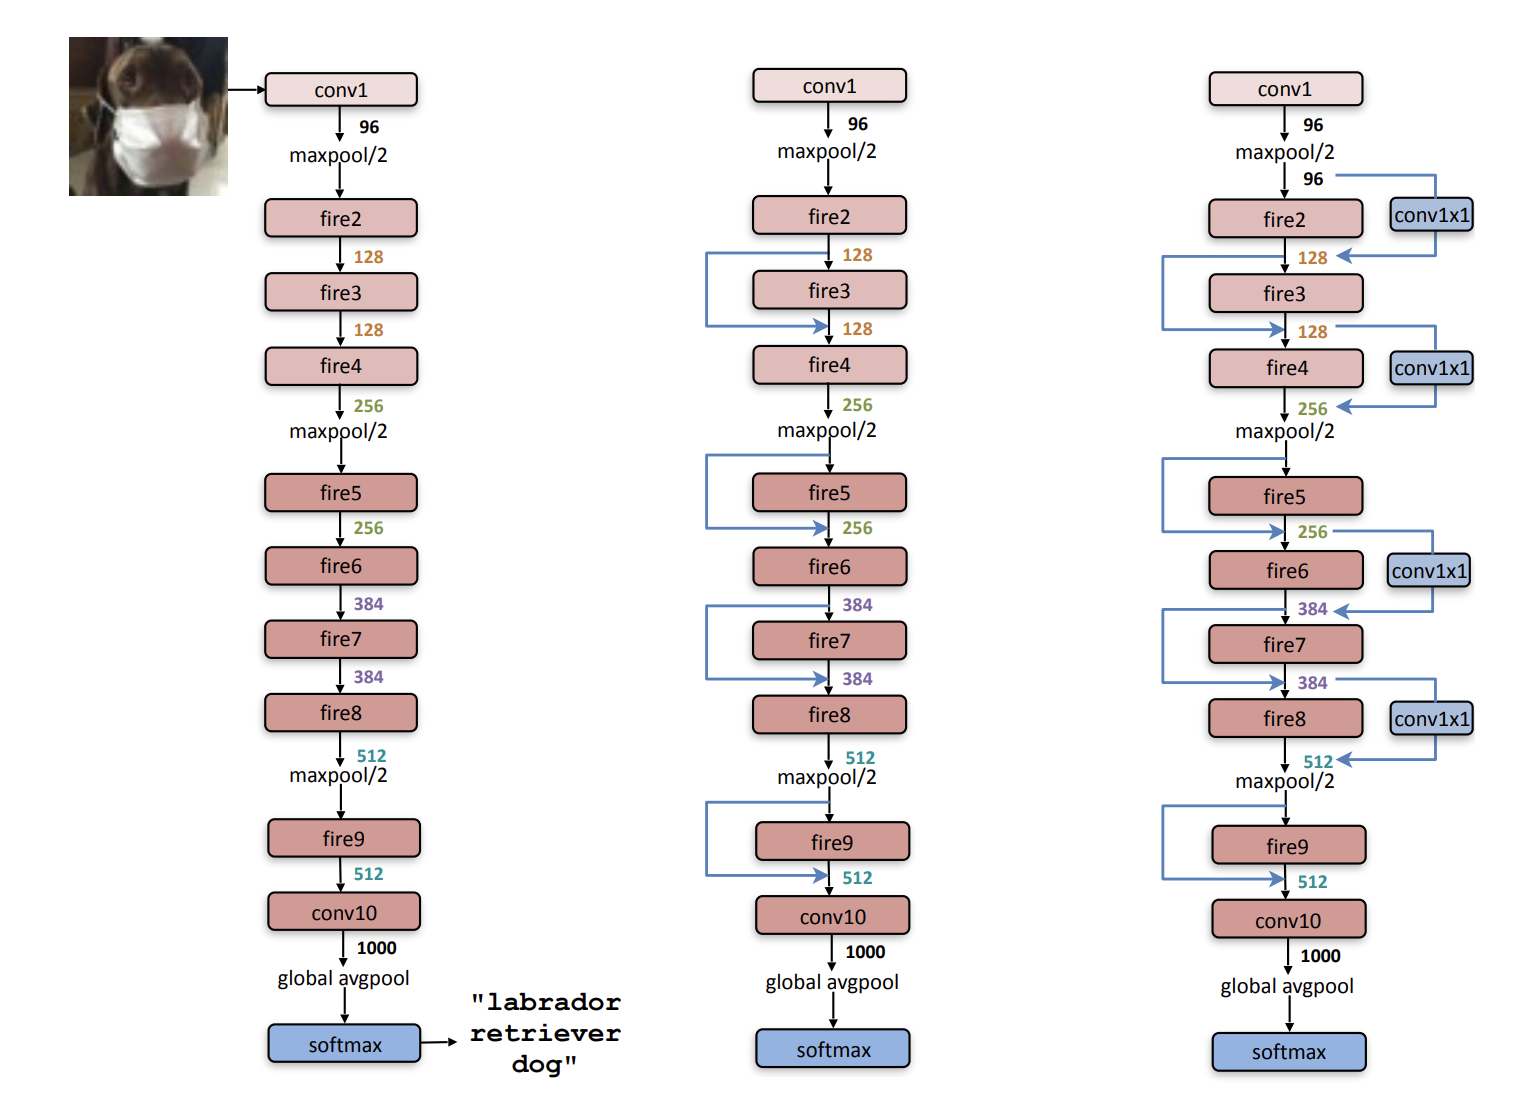
\includegraphics[scale = 0.2]{imagenes/squeezenet.png}
	\caption{Arquitectura de SqueezeNet}
\end{figure}


Esta red ha sido empleada en multitud de aplicaciones: detección de objetos en tiempo real, clasificación semántica, y modelos preliminares de conducción autónoma. Entre todas sus aplicaciones, podríamos destacar su utilización en imagen médica, concretamente MRI (Resonancias magnéticas). Ha permitido facilitar el diagnóstico de ciertas enfermedades y lesiones cerebrales en un espacio de memoria y recursos contenido.\\

Sin embargo, a pesar de las mejoras recibidas en sus versiones sucesivas, como los módulos Fire de doble nivel para reducir dimensionalidad, o la introducción de más reducciones mediante pooling, sacrifica resultados a nivel de accuracy respecto a la competencia, y no ha sido aplicada de forma firme y exitosa sobre imágenes de enfermedades cutáneas.



\subsection{MobileNet}

MobileNet es el fruto del proyecto de investigación de Google Research para la implementación de redes convolucionales en dispositivos móviles. El objetivo era encontrar un modelo eficiente que pueda ser incluso utilizado en tareas de segmentación en tiempo real, pero reduciendo el número de parámetros del red así como el número de operaciones de producto necesarias, para poder ejecutarlas de forma nativa en dispositivos móviles como smartphones y tablets.\\

Esta arquitectura consta de 3 versiones diferentes, siendo cada una más sofisticada que la anterior. Disponemos de MobileNet V1, MobileNet V2 y MobileNetV3.

\subsubsection{MobileNet V1 (2017)}

La versión original de la arquitectura convolucional MobileNet  \cite{howard2017mobilenets} fue publicada en 2017. En esta publicación, se busca reducir el número de operaciones realizadas para conseguir un menor impacto de las operaciones en punto flotante sobre el rendimiento.\\
El punto clave de esta arquitectura reside en las llamadas "pointwise convolutions", haciendo uso del concepto de separabilidad, ampliamente estudiado desde el año 2012 por la literatura.

Las nuevas convoluciones descomponibles se pueden separar en dos pasos bien delimitados: la convolución en profundidad y la convolución puntual.

\begin{itemize}
    \item Las convoluciones en profundidad realizan el producto del filtro con el volumen de entrada capa a capa. Es decir, no se tiene en cuenta la dimensionalidad total de la imagen, sino que se realiza por cada nivel de profundidad el mismo producto. Esto reduce considerablemente el número de parámetros, ya que la dimensionalidad del problema es mucho menor.
    \item La segunda fase es la convolución puntual, cuyo objetivo no es más que acumular el producto de todas las capas calculadas independientemente mediante una simple combinación lineal, la cual es de coste computacional muy bajo.
    
    $$G_{k,l,m} =  \sum_{i,j}^{} K^{i,j,m} * F_{k+i-1,l+j-1,m}$$
\end{itemize}

Este producto es calculable eficientemente por las técnica de álgebra lineal GEMM, que permite aplicar propiedades de la suma y la multiplicación para el producto matricial de forma eficiente mediante Tensor cores.\\

En resumen, gracias a la separabilidad convolucional, se adquieren varias ventajas:
\begin{itemize}
    \item El número de productos se reduce considerablemente. Como se puede verificar en \cite{howard2017mobilenets} se traduce en una reducción de entre 8 y 9 veces el número de operaciones con respecto a las arquitectura tradicional de convolución
    \item Se reduce el espacio necesario en memoria.
    \item Se puede aprovechar el hardware específico.
    \item No se pierde precisión de cálculo gracias a que la separabilidad de convoluciones no afecta al resultado.
\end{itemize}

\begin{figure}[H]
	\label{depthwise}
	\centering
	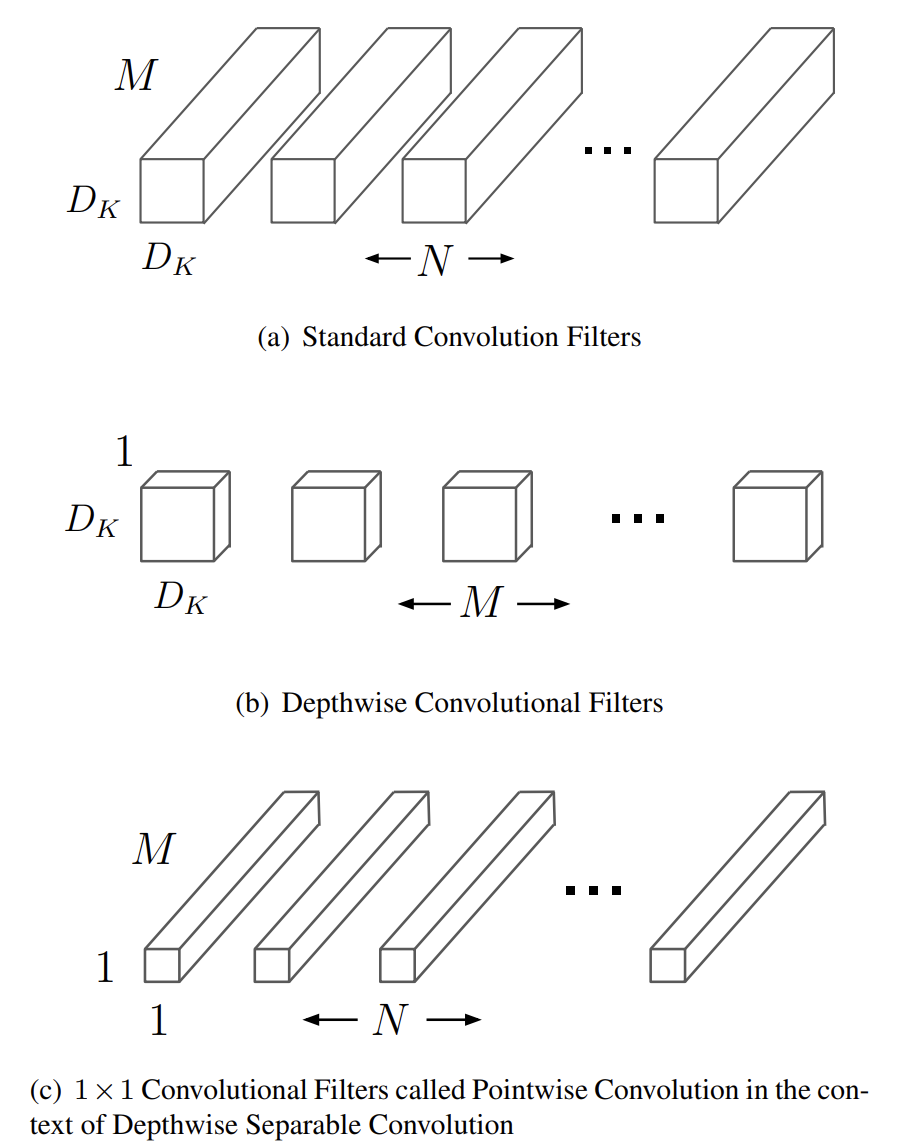
\includegraphics[scale = 0.225]{imagenes/depthwise.png}
	\caption{Producto depthwise}
\end{figure}

Adicionalmente, también incorporaron dos hiperparámetros: $\alpha$ y $\rho$. Estos parámetros controlan la anchura y la resolución de entrada, respectivamente.\\
El hiperparámetro $\alpha$ hace referencia a la anchura de cada capa convolucional que compone la red, adquiriendo un valor de 1 cuando la arquitectura no se ve reducida, y gradualmente podrá ser reducida en el intervalo (0,1]. Así se conseguirán modelos más simples en anchura para dispositivos con menores recursos.\\

En cuanto a $\rho$, este se encuentra implícito en la resolución de la imagen de entrada. Por defecto, la red acepta imágenes de hasta 224x224, pero en función de dicho valor $\rho$, podremos reducir su resolución también dentro del intervalo (0,1].\\

Ambos parámetros sacrificarán bondad y ajuste en los resultados a favor de una mayor eficiencia.

\subsubsection{MobileNet V2 (2018)}

Dos años más tarde de la publicación de MobileNets, da a luz su versión V2  \cite{sandler2019mobilenetv2}. Esta conserva los hiperparámetros  de la versión anterior, así como el producto punto a punto. Sin embargo, añade tres nuevas características, algunas de ellas no triviales y que requieren experimentación:
\begin{itemize}
    \item Se introduce el concepto de ``residuo invertido''. Ésta mejora reside en la utilización de los bloques residuales, propuesto por la arquitectura de ResNet. Su objetivo es evitar la degradación del gradiente, y que se frene el aprendizaje en modelos de gran profundidad. Normalmente, estas conexiones se realizan entre capas de gran profundidad, siendo las capas intermedias bloques estrechos. Sin embargo, en MobileNet V2, se propone la composición inversa, de forma que sean los bloques intermedios entre los residuales aquellos que poseen una mayor anchura, y así reducir el número de parámetros sin perder expresividad en el modelo \cite{invertedresidualsv2}.
    \begin{figure}[H]
    	\label{invert}
    	\centering
    	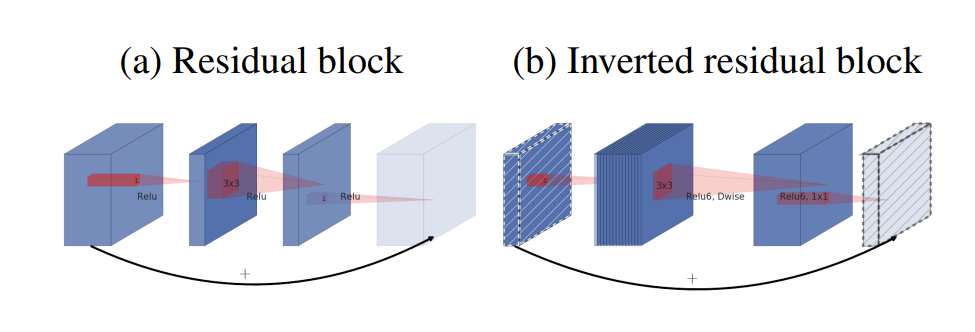
\includegraphics[scale = 0.3]{imagenes/invertedres.png}
    	\caption{Bloque residual invertido}
    \end{figure}
    
     \item En las capas donde el volumen de entrada es estrecho, al hacer uso de bloques residuales invertidos, la eliminación de la no linealidad aportada por ReLu favorece a la conservación de características y permite obtener mejores resultados de accuracy en tareas generales como clasificación en imagenet. Esto se debe a que al realizar los saltos entre bloques ``estrechos'' perdemos rendimiento de la red, y simplemente con eliminar la última transformación no lineal del bloque, contrarrestamos este problema.
    \item ReLu6. Se mantiene una versión modificada de la original función de activación. En lugar de utilizar la tradicional función ReLu entre 0 y 1, se extiende este intervalo hasta 6, permitiendo mantener la precisión en caso de utilizar coma fija, ya que se aseguran 3 dígitos de parte entera, y el resto queda destinado a la mantisa, que se almacena de forma precisa.
\end{itemize}

    \begin{figure}[H]
	\label{mv2}
	\centering
	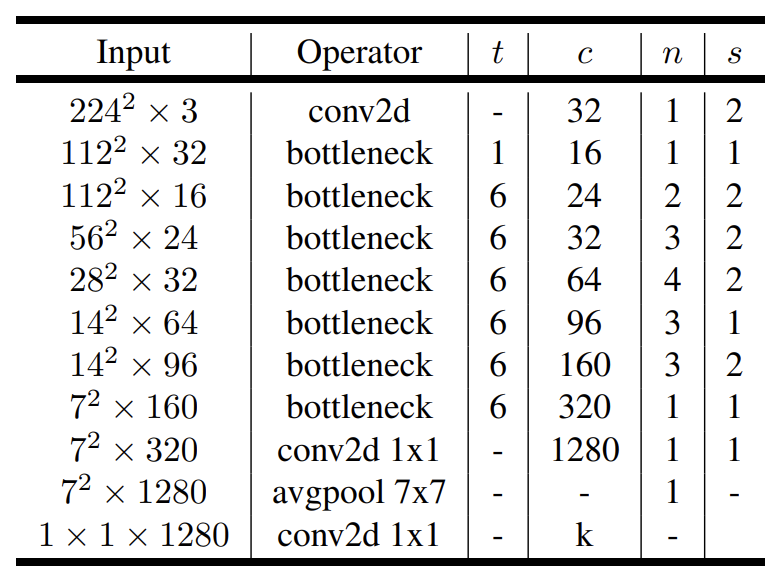
\includegraphics[scale = 0.25]{imagenes/mobilenetv2.png}
	\caption{Arquitectura de MobileNetV2}
\end{figure}

\subsubsection{MobileNet V3 (2019)}

En su tercera versión\cite{howard2019searching}, MobileNet incorpora métodos avanzados de diseños de redes basados en NetAdapt. Este algoritmo se basa en la transformación de modelos preentrenados para escritorio, y, en base a una serie de requisitos de potencia especificados, adapartar la arquitectura a una plataforma móvil perdiendo las mínimas capacidades posibles de la red original.  El modelo de partida empleado fue ajustado con precisión para mejorar latencias y uso de memoria, aplicando los siguientes conceptos:

\begin{itemize}
    \item Se añade la capa Squeeze-and-Excite, dentro de las conexiones residuales. Se trata de un mecanismo surgido en 2018 \cite{hu2019squeezeandexcitation}. Este estudio afirma que existen filtros de imagen con mayor importancia para el cómputo global que otros, como, por ejemplo, los bordes. Por tanto, les aporta un mayor ``peso'' durante el entrenamiento a dichos filtros haciendo uso de una serie de parámetros adicionales. Éstos añaden una carga computacional muy pequeña, por lo que se trata de una técnica eficaz. Para obtener los parámetros de relevancia, se dispone de dos módulos: squeeze, y excite. El módulo squeeze se encarga de representar cada filtro mediante un valor numérico, obtenido por average pooling de la imagen. Y por otro lado, el módulo excite se encarga de aprender los pesos que dar a cada uno de estos filtros o canales, haciendo uso de un MLP. El resultado final serán los pesos de cada canal en cuanto a su importancia, normalizados entre 0 y 1 por una función sigmoide.

    \item Se incluyeron nuevas capas al inicio y al final de la red de tipo residual invertidas.
\end{itemize}

    \begin{figure}[H]
	\label{mv2}
	\centering
	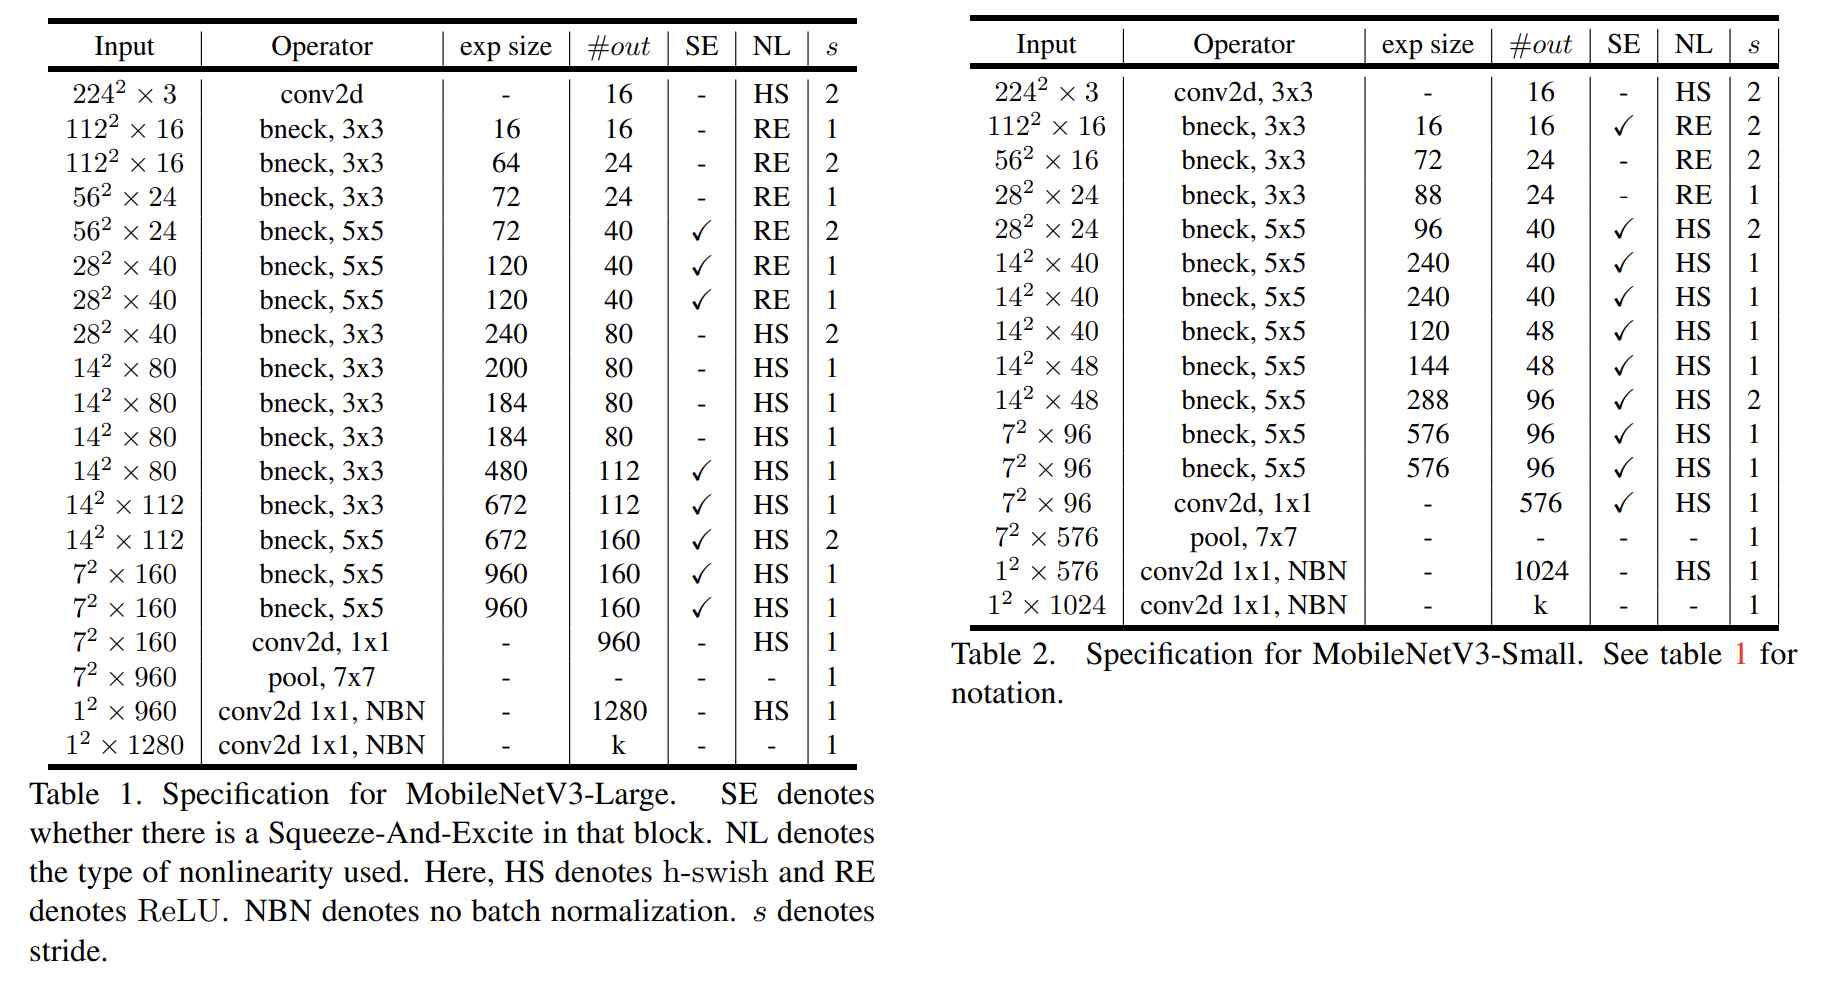
\includegraphics[scale = 0.85]{imagenes/mobilev3.png}
	\caption{Arquitectura de MobileNetV3}
\end{figure}

Debido a la gran complejidad adquirida por el modelo, los problemas de latencia y rendimiento en dispositivos de menor potencia, se opta por dividir la arquitectura en dos modelos parametrizables: MobileNet Small y Large. Mientras que la versión Large mejora los resultados de la versión 2 aumentando las prestaciones, el modelo Small otorga importancia sobre todo a la eficiencia y el uso de memoria, enfocado al hardware embebido o dispositivos de poca potencia.


\subsubsection{Aplicaciones en dermatología y cáncer de piel}

MobileNet, concretamente en su segunda versión, ha sido utilizado en la literatura para el diagnóstico de enfermedades de la piel. En \cite{Chaturvedi_2020}, es utilizado para realizar la clasificación de 7 enfermedades cutáneas extraídas del Humans against Machine, HAM10000 \cite{ham10000}, que podemos encontrar en ISIC archive \cite{isicarchive}, un repositorio web de acceso libre con enfermedades de la piel tanto beningnas como cancerosas. 

También se utilizó más recientemente para su implementación en dispositivos de IOT, \cite{mnetsqueeze}, donde se logra alcanzar el 99\% de accuracy en un pequeño conjunto extraido de ISIC, haciendo uso de la versión V3 junto a un algoritmo de Squeeze. Dicho algortimo se encarga de localizar la ubicación de los pelos y otros posibles artefactos para preprocesar la imagen y lograr una fotografía resultante libre de interferencias. 

Para ello, hace uso de un filtro black hat, que binariza la imagen y obtiene los píxeles objetivo de eliminar, que son sustituidos por los colores de los píxeles adyacentes, junto al uso del aumento de datos. Sin embargo, no queda especialmente claro la tasa de precisión del modelo para cada una de las enfermedades que se intentan diagnosticar.

\subsection{Shuffle Net}

Shuffle Net \cite{zhang2017shufflenet,shufflenetreview} surge con el objetivo ofrecer un modelo capaz de ofrecer un buen modelo con la mínima pérdida de rendimiento frente a modelos profundos. Es capaz de superar en resultados a la primera versión de MobileNet, logrando un error de aproximadamente tres puntos menos que MobileNet V1. Su mejor rendimiento se debe sobre todo al uso de Channel Shuffle para las convoluciones grupales, y creando una arquitectura basada en módulos shuffle.

La convolución en grupo mediante mezcla de canales (Channel Shuffle) surge tras el estudio del funcionamiento de las convoluciones grupales en 	AlexNet\cite{NIPS2012_c399862d} y ResNext. En ambos modelos, se uitilizan convoluciones grupales, donde cada canal de salida sólo se relaciona con los canales de entrada del que proviene. Esto podría debilitar la relación entre cada canal, y debilitar los resultados; para evitarlo, y no poner en riesgo el rendimiento con demasiadas convoluciones 1x1 para relacionarlos, se hace uso del mezclado de canales; es decir, es como si permitiésemos que cada grupo convolucional pudiera obtener información de otros grupos adyacentes, para así mejorar la relación entre ellos.

Para evitar un sistema complejo a la hora de representar dichas interconexiones, es como surge el channel shuffle \ref{shufflechannels}: se mezclan los canales de forma que los grupos ya no quedan aislados con sus respectivas entradas y salidas.

    \begin{figure}[H]
	\label{shufflechannels}
	\centering
	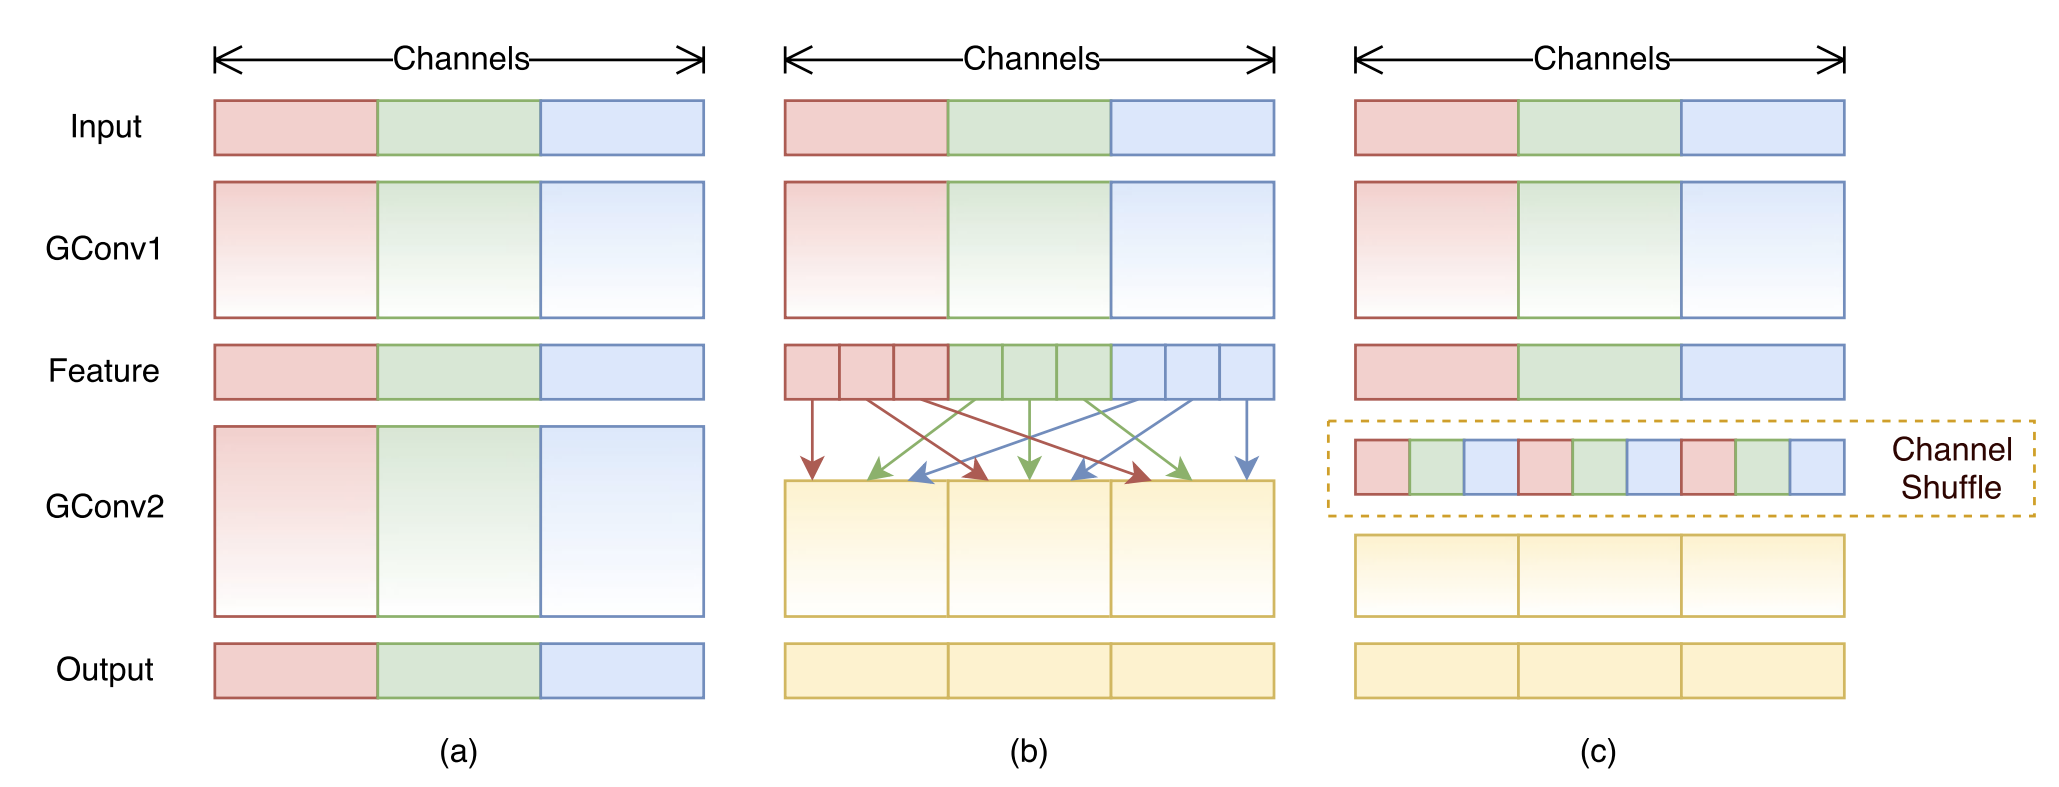
\includegraphics[scale = 0.2]{imagenes/shufflechannels.png}
	\caption{Channel Shuffle de ShuffleNet}
\end{figure}

Esta técnica se aplicará sobre la primera y última convolución 1x1 realizada sobre los bloques residuales de la red, que siguen una estructura parecida a la que adoptaría MobileNetV2 posteriormente. Mediante esta propuesta, podemos además aplicar una mayor capacidad de procesamiento en anchura añadiendo stride, y aplicando average pooling. El resultado, es conseguir modelos más anchos en procesamiento que no impacten negativamente en el rendimiento de los dispositivos con menor capacidad. En la figura \ref{label} , podemos apreciar la arquitectura de la red, cuyos filtros pueden ser escalados mediante el parámetro s, aunque teniendo en cuenta una penalización en la complejidad, equivalente a $s^2$ sobre Shuffle Net base, equivalente a $s=1$

\begin{figure}[H]
		\label{arquitecturashuffle}
		\centering
		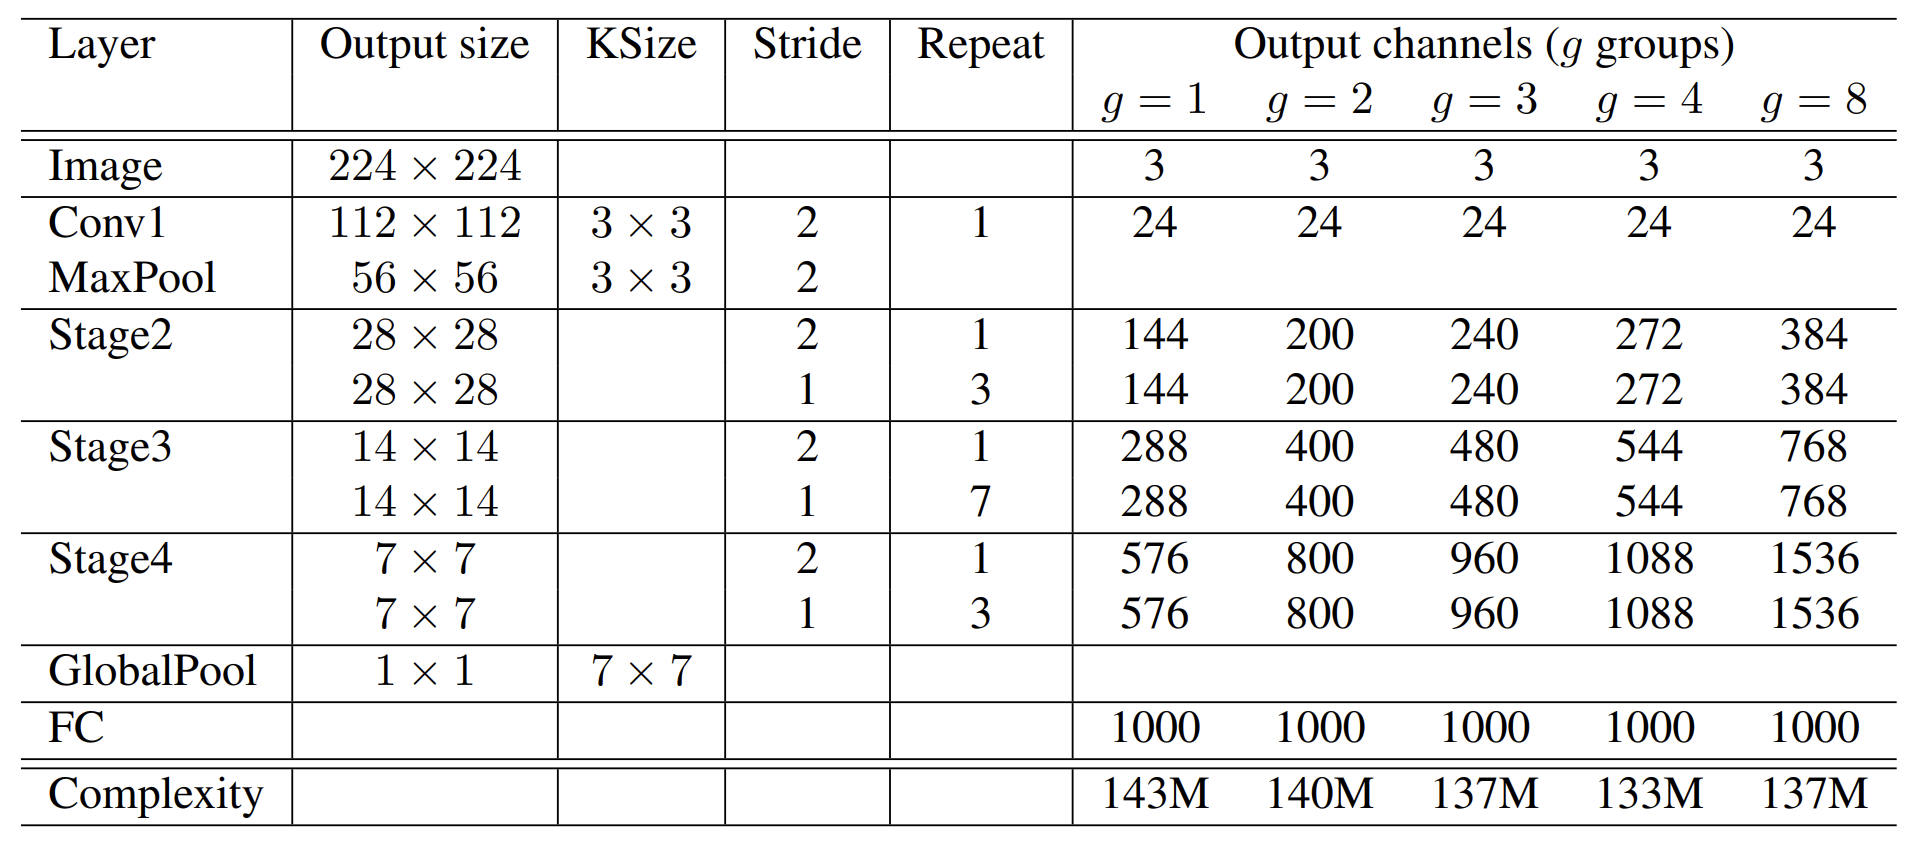
\includegraphics[scale = 0.2]{imagenes/arquitecturashuffle.png}
		\caption{Arquitectura de ShuffleNet}
	\end{figure}

Sus aplicaciones han sido variadas, pero en lo que respecta a la detección de lesiones cutáneas, la cercana salida de MobileNet V2 y su mejor rendimiento provocó que ShuffleNet quedase relegada a un segundo plano, y no fuese muy utilizada para este fin. Podemos encontrar algunos trabajos \cite{shuffleapp} donde podemos observar una comparativa de este modelo frente a la completitud de los modelos del estado del arte de 2022, y podemos confirmar que  MobileNetV2 es capaz de superar su rendimiento en la mayoría de pruebas, siendo estas comparaciones en cuanto a tiempo de entrenamiento, precisión, accuracy y tamaño del conjunto de entrenamiento. Sólo consigue superar a MobileNetV2 en tiempo de entrenamiento, donde es aproximadamente 900 más rápida, pero ofrece peores resultados en promedio.

\subsection{EfficientNet lite}

EfficientNet \cite{Chaturvedi_2020} es un conjunto de arquitecturas de redes creadas por el departamento de investigación de Google con el fin de conseguir una familia de modelos variada que fuese capaz de adaptarse fácilmente mediante parámetros a diferentes conjuntos de imágenes, y a requisitos de hardware más o menos limitados. 

Parte de que una red convolucional sigue el siguiente esquema:
$$\mathcal{N}=\odot_{i=1...s} F_i^{L_i}(X_{(H_i, W_i,L_i)})$$


Donde se denota que la capa $F_i$ es repetida $L_i$ veces la etapa i de la red, y la dimensionalidad de la capa queda representada con ${( W_i,L_i)}$.  Fijando $F_i$, efficient net intenta dar versatilidad a sus modelos variando las dimensiones restantes, Li, Ci, Hi, Wi mediante el uso de 3 constantes de escalabilidad:

\begin{itemize}
	 \item  Profundidad, Depth (d):  Aumentar la profundidad es la tendencia habitual presente en las redes convolucionales. Pero llegar a un equilibrio es crítico, ya que aumentar demasiado la profundidad sin modificar otros parámetros puede ocasionar pérdidades rendimiento por el desvanecimiento del gradiente  a menor profundidad. 
	\item Anchura, Width (w): Aumentar la anchura suele ser beneficioso para modelos de pocos recursos donde el aumento de profundidad supone un gran aumento de la carga computacional. Permite conseguir mayor cantidad de características de grado fino, pero si la red es demasiado poco profunda, el modelo careceré de características de alto grado que permitan aprender patrones generales.
	\item Resolución, (r): al emplear tamaños de entrada mayores, damos opciones a obtener una mayor cantidad de características de grado fino, pero un exceso de resolución puede provocar grandes tiempos de ejecución y puede ser contraproducente, al reducirse la ganancia con tamaños demasiados grandes.
\end{itemize}

\begin{figure}[H]
	\label{arquitecturashuffle}
	\centering
	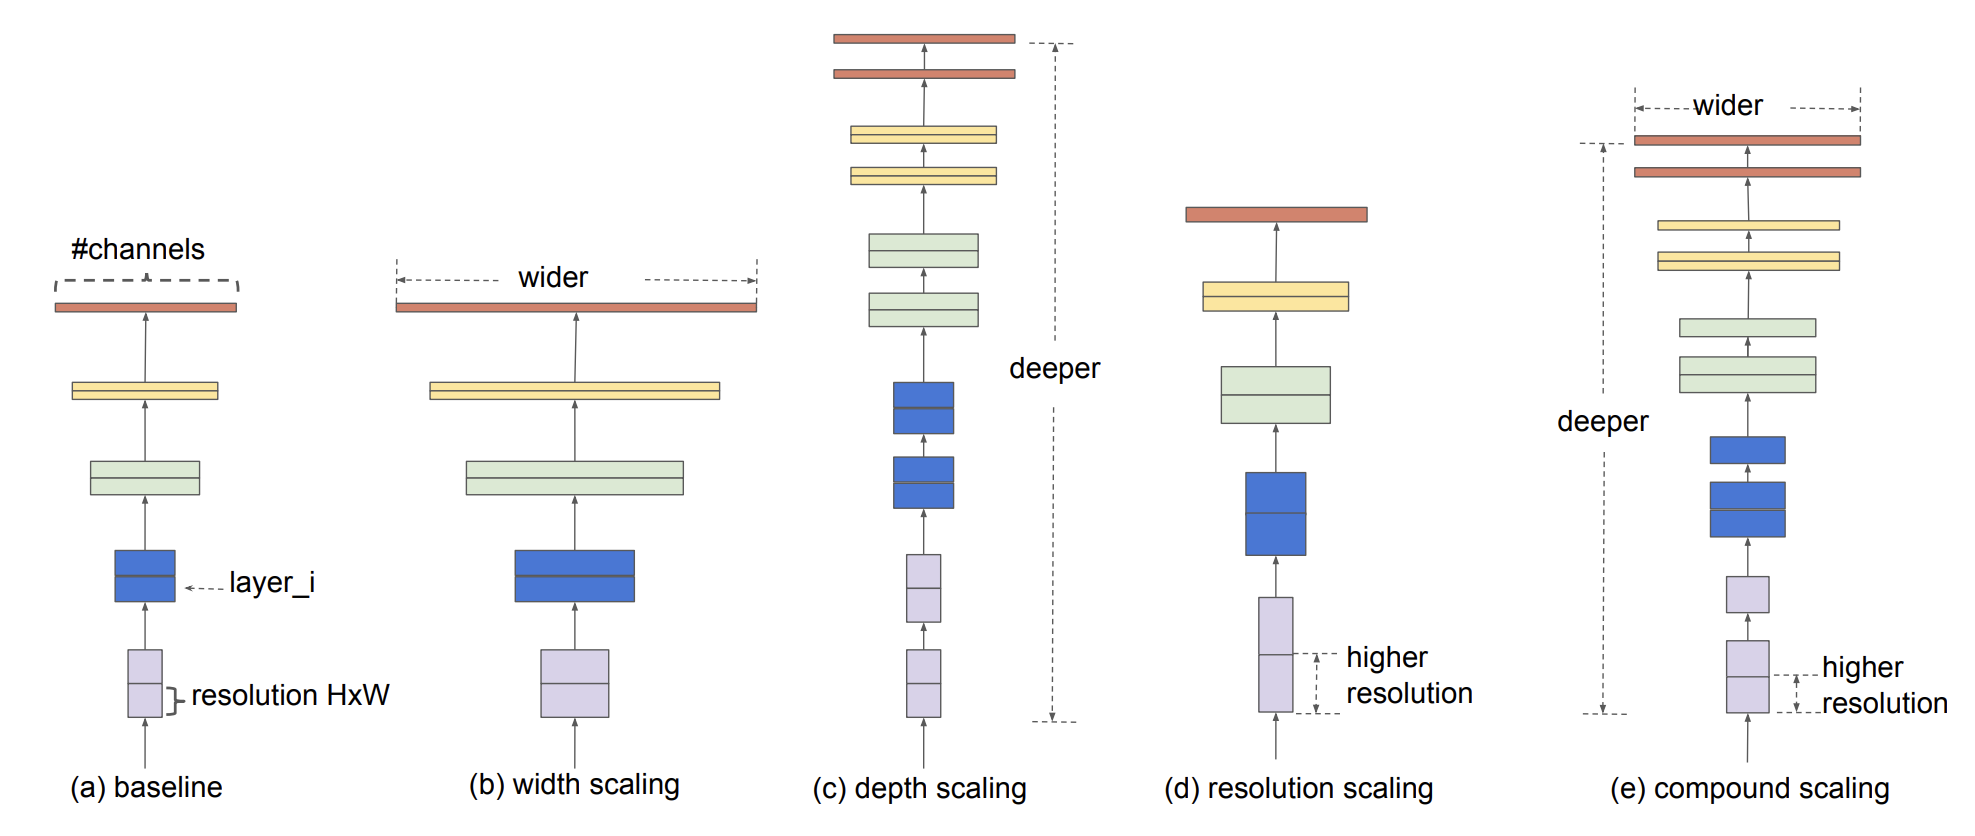
\includegraphics[scale = 0.2]{imagenes/efnet_scale.png}
	\caption{Parámetros de EfficientNet}
\end{figure}


Experimentalmente, estos parámetros pueden ser ajustados, y dan lugar a una serie de modelos distinto: los conocidos EfficientNetB0 - B7, denotando el valor numérico la profundidad y complejidad del modelo, siendo esta mayor a mayor valor del índice.	 Cada una de ellas fue ajustada utilizando como requisito la potencia medida en TFLOPS para su ejecución, y puede ser posteriormente ajustada con el resto de parámetros libres no fijados a las características del conjunto de entrada.\\


\subsubsection{Aplicaciones en dermatología y cáncer de piel}

En el problema que nos concierne, esta arquitectura ha conseguido grandes resultados en el dataset del ISIC abierto al público como competición en la plataforma Kaggle, habiendo sido utilizado como parte de un ensemble de modelos, o bien como modelo único entrenado en el top 3 de ganadores de la competición. En el caso de la segunda mejor solución clasificada \cite{2ndISIC}, se menciona la utilización de EfficientNet-B6, con tamaño de entrada de 512x512, y un tamaño de batch de 64, obteniendo 0.9485 de accuracy como resultado final a la hora de emplear los datasets ISIC 2019 y 2020\\ En la primera solución, es usada en conjunto a Resnet50, y una red especializada en los metadatos de la imagen, y todos los modelos juntos someten su resultado a votación \cite{1stISIC}.

Ambos resultados han sido evaluados con computadores de alta gama, haciendo uso de múltiples tarjetas gráficas para el entreanmiento y la inferencia. Este proceso es demasiado pesado para un dispositivo móvil, por lo que de cara a este trabajo, se buscarán alternativas capaces de ahorrar en espacio y potencia como concepto de cuantización.

 \subsection{Cuantización de modelos}


\section{Recursos gráficos disponibles}

La obtención de datos es un proceso fundamental en la resolución de problemas de Machine Learning. Este tipo de problemas requieren un gran número de imágenes que aporten variedad, y permitan construir un modelo general que se capaz de adaptarse a cambios de iluminación, diferentes puntos de vista y composiciones.

Es clave, por tanto, disponer de diferentes tipos de lesiones, tanto benignas como malignas, así como diferentes tonos de piel. La inexistencia de un tipo de piel en el conjunto de entrenamiento, o la inexistencia de un tipo de lesión podrían provocar resultados sesgados indeseados durante la predicción de la imagen tomada.

Podemos encontrar en la red varios datasets de acceso público que permiten su utilización de forma abierta con fines académicos. Dada a la gran cantidad de publicaciones disponibles, resulta complejo averiguar si los datos a los cuales hace referencia se encuentran disponibles públicamente, si son de acceso restringido, o bien, ya no se encuentran disponibles debido a cambios en su política o la falta de mantenimiento.

Debido a que el estudio de la evolución y el diagnóstico del cáncer de piel de forma temprana es un tema en auge, existen gran cantidad de publicaciones especializadas únicamente en el análisis de los conjuntos de datos públicamente accesibles, como es el caso de la lista propuesta por M. Goyal et Al. [16], o el reciente estudio realizado por Sana Nazari y Rafael García (2023)[30].
Basados en su modelo de estudio y las referencias recomendadas por sus artículos, se ha elaborado el siguiente plan de búsqueda para saber qué tipo de datos utilizar y cuáles descartar:

\begin{figure}[H]
	\centering
	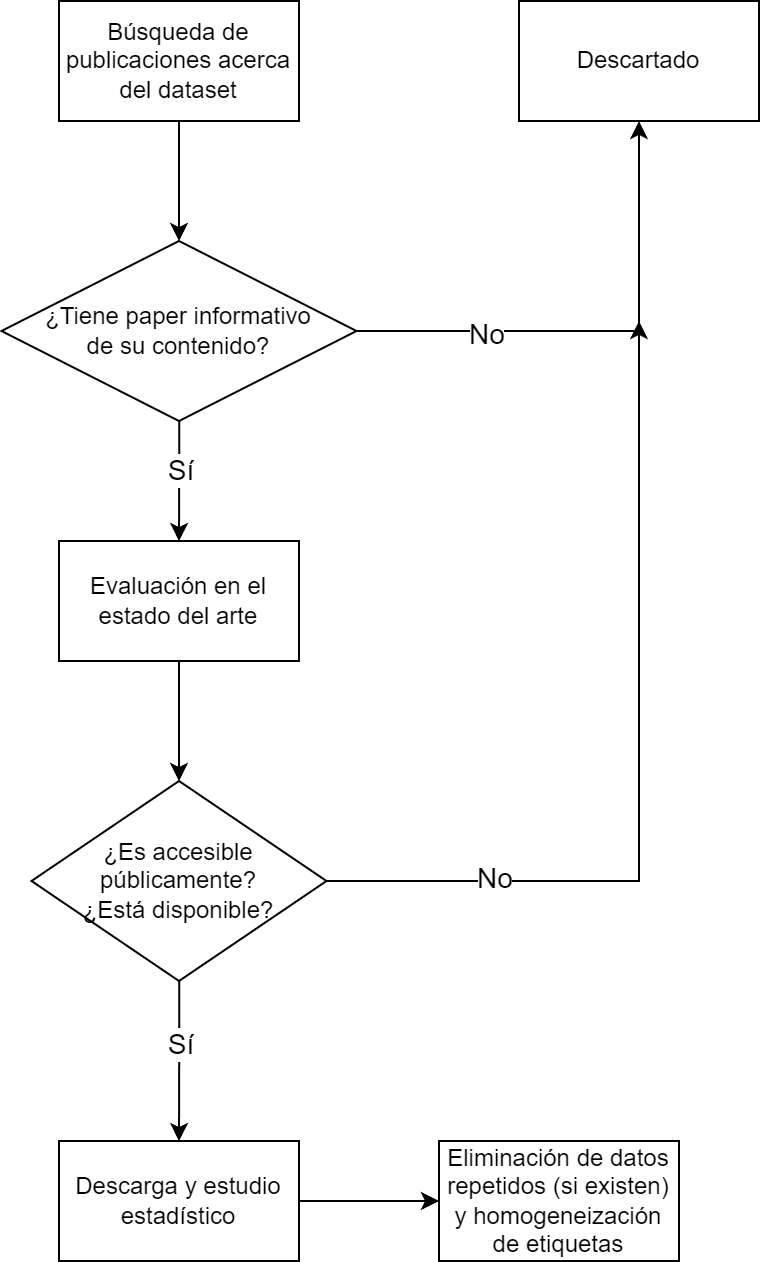
\includegraphics[scale=0.75]{imagenes/DiagramaBusqueda.png}
	\caption{Proceso de búsqueda seguido}
\end{figure}

Siguiendo dicho procedimiento, se han encontrado 6 datasets diferentes, cuyo origen son instituciones públicas que han cedido datos con fines académicos y de investigación.\\

Un factor determinante para la elección de estos conjuntos es la diversidad. Es indispensable, para este proyecto, encontrar datos lo suficientemente variados como para distinguir lesiones cancerígenas y no cancerígenas, y disponer de diferentes tonos de piel para entrenar. Aunque los tonos de piel más oscuras sufren lesiones de tipo cancerígeno en menor proporción gracias a su protección natural, también pueden sufrir este tipo de patologías, y es clave ser capaces de detectarlas en cualquier posible paciente.

\subsubsection{ISIC Data}
El repositorio ISIC (International Skin Imaging Collaboration [1]), contiene imágenes demoscópicas de lesiones principalmente cancerosas.  Existe una gran cantidad de publicaciones acerca de este conjunto de datos, debido a su utilización anual durante los años 2016-2020 para la realización de un reto virtual de Machine Learning descrito en [1]. El objetivo, consiste en identificar los melanomas frente a lesiones no cancerosas (ISIC Challenge-2020[2]) o bien, identificar diferentes subtipos de lesiones cancerosas frente a lesiones benignas (ISIC Challenge 2019, [3]). \\

En el estado del arte, destacan las soluciones que hacen uso de métodos de DeepLearning, como el planteado por Ian Pan [4], finalista de la competición para el año 2020. El ganador de la competición del año 2020, cuyo análisis podemos encontrar en [5], realiza por su parte un enfoque híbrido entre el uso de DeepLearning para la clasificación de los datos de tipo imagen, y clasificación mediante Machine Learning para los metadatos, y así obtener un resultado más preciso. \\

Debido a que cada uno de estos subconjuntos de datos anuales podían ser pequeños, normalmente se recurría a la reutilización de los conjuntos anteriores para enriquecer el conjunto de entrenamiento.  Este método es bastante recomendable, ya que, a mayor conjunto de entrenamiento, más cercanos se encontrarán los parámetros de interés del problema general a solucionar. Sin embargo, hay que realizar dicha fusión con especial cuidado, ya que existen volúmenes de datos considerables que se repitieron en las competiciones de cada año para aumentar el tamaño del dataset, y si se realizase una simple concatenación de los datos, estaríamos desperdiciando esfuerzo computacional en clasificar imágenes redundantes (comportamiento para nada deseable al trabajar sobre entornos móviles de menor potencia.).\\

Un análisis extenso de los datos asociados a cada Challenge podemos encontrarlo en [6]. En él, se recogen otros modelos del estado del arte utilizables para este fin, así como una forma de tratar los datos duplicados. Los datos pueden ser separados en los siguientes subconjuntos:

\begin{table}[H]
	\centering
	\begin{tabular}{|l|l|l|l|l|}
		\hline
		\textbf{Challenge Dataset Year} & \textbf{Train} & \textbf{Test} & \textbf{Total} & \textbf{Tipo de problema } \\ \hline
		ISIC 2016 & 900 & 379 & 1279 & Clas. binaria  \\ \hline
		ISIC 2017 & 2000 & 600 & 2600 & Clas. Multiclase  \\ \hline
		ISIC 2018 & 10015 & 1512 & 11527 & Clas. Multiclase  \\ \hline
		ISIC 2019 & 25331 & 8238 & 33569 & Clas. Multiclase  \\ \hline
		ISIC 2020 & 33126 & 10982 & 44108 & Clas. Binaria  \\ \hline
	\end{tabular}
\end{table}

\begin{itemize}
	
	\item ISIC 2016 [7]:  Es el dataset de menor tamaño de todos los propuestos. Hace distinción únicamente de los casos malignos y benignos. Contiene imágenes dermoscópicas anotadas con información acerca de la localización de la mancha, y la edad del paciente. Contiene información adicional para la segmentación de la mancha pigmentada de interés (máscaras).
	\item ISIC 2017 [8] Es un conjunto de mayor tamaño al anterior, y hace alusión a 4 clases diferentes: melanomas, nevus, y seborrheic keratosis. Contiene también información acerca de la edad del paciente, y otros metadatos de interés. La escasa cantidad de datos provoca que normalmente en la literatura este dataset se utilice también como clasificación binaria entre nevus y keratosis, u otros enfoques similares. 
	\item ISIC 2018 [9]. Este dataset contiene un número de imágenes considerables, siendo un total de 10015 imágenes para entrenamiento, y 1512 para test. En este caso, se realiza subclasificación de tipos, a través de las clases melanocytic nevus, basal cell carcinoma, actinic keratosis, benign keratosis, dermatofibroma y lesiones vasculares. Es de especial interés destacar que este dataset proviene, a su vez, de HAM10000 (Human against machine, [11] )  y MSK Dataset [12]. El challenge original comprendía, de nuevo, la clasificación de los diferentes tipos realizando previamente una discriminación de la mancha en cuestión mediante segmentación. Existen gran cantidad de publicaciones que tratan este conjunto de datos, como [13], donde se emplea este dataset para demostrar mejores resultados al emplear transformaciones polares de la imagen y aumentar la invarianza.
	
	\item ISIC 2019 [2].  Se trata del mayor conjunto de datos para clasificación multiclase propuesto por ISIC [1]. Se trata del mismo dataset que el año 2018 [9], con la adición de BCN\_20000 Dataset [14], cuyos datos provienen del Hospital Clínic de Barcelona [14]. Las clases a clasificar se amplían hasta 9, encontrando subtipos de melanomas en el conjunto.
	\item ISIC 2020 [3]. El último dataset propuesto públicamente, contiene únicamente datos binarios acordes a melanomas y no malignos. 
\end{itemize}

Todos estos datos pueden ser acoplados entre sí para dar un dataset global de ISIC [6], donde obtendríamos las siguientes clases: 


\begin{table}[H]
	\centering
	\begin{tabular}{|c|c|c|c|c|}
		\hline
		\textbf{Clase} & \textbf{2017} & \textbf{2018} & \textbf{2019} & \textbf{2020} \\ \hline
		\textbf{Melanoma} & 374 & 1113 & 4522 & 584 \\ \hline
		\textbf{Atypical melanocytic proliferation} & - & - & - & 1 \\ \hline
		\textbf{Cafe-au-lait macule} & - & - & - & 1 \\ \hline
		\textbf{Lentigo NOS} & - & - & - & 44 \\ \hline
		\textbf{Lichenoid keratosis} & - & - & - & 37 \\ \hline
		\textbf{Nevus} & - & - & - & 5193 \\ \hline
		\textbf{Seborrheic keratosis} & 254 & - & - & 135 \\ \hline
		\textbf{Solar lentigo} & - & - & - & 7 \\ \hline
		\textbf{Melanocytic nevus} & - & 6705 & 12.875 & - \\ \hline
		\textbf{Basal cell carcinoma} & - & 514 & 3323 & - \\ \hline
		\textbf{Actinic keratosis} & - & 327 & 867 & - \\ \hline
		\textbf{Benign keratosis} & - & 1099 & 2624 & - \\ \hline
		\textbf{Dermatofibroma} & - & 115 & 239 & - \\ \hline
		\textbf{Vascular lesion} & - & 142 & 253 & - \\ \hline
		\textbf{Squamous cell carcinoma} & - & - & 628 & - \\ \hline
		\textbf{Other / Unknown} & 1372 & - & - & 27.124 \\ \hline
		\textbf{Total} & 2000 & 10.015 & 25.331 & 33.126 \\ \hline
	\end{tabular}
\end{table}

Sin embargo, sería necesario tener en cuenta la eliminación de imágenes repetidas, debido a que durante cada edición de ISIC, un número considerable de imágenes han sido incluidos en varios años. Este procedimiento engloba:

\begin{enumerate}
	
	
	\item Eliminar las imágenes idénticas por hash. Todas las imágenes de ISIC están numeradas de forma única para facilitar la identificación de cada una de ellas. Si unimos todos los datatesets, y tomamos las repeticiones, podemos remover:
	
	\begin{table}[H]
		\centering
		\begin{tabular}{|c|c|c|c|c|c|}
			\hline
			\textbf{} & \textbf{2016} & \textbf{2017} & \textbf{2018} & \textbf{2019} & \textbf{2020} \\ \hline
			\textbf{Train} & 291 & 1283 & 0 & 0 & 0 \\ \hline
			\textbf{Test} & 95 & 594 & 0 & 0 & 0 \\ \hline
		\end{tabular}
		\caption{Número de imágenes duplicadas recogidas por [6]}
	\end{table}
	
	
	\item 	Eliminación del ISIC 2018. Como éste se encuentra contenido en la composición para el año 2019, puede prescindirse totalmente de él a favor de la versión de 2019.
	\item 	Eliminación de imágenes “downsampled” del conjunto. En los años 2019 y 2020, se añadieron imágenes de challenges anteriores con una reducción en resolución. Para ahorar en espacio y tiempo de cómputo, pueden eliminarse las imágenes reducidas para quedarnos con una única copia de mayor calidad de la lesión, y luego realizarles manualmente un reescalado en caso de que sea necesario.
	
	Atendiendo de nuevo a los resultados propuestos por [6], obtenemos el siguiente conjunto: 
	
	\begin{table}[H]
		\centering
		\begin{tabular}{|c|c|c|c|}
			\hline
			\textbf{Year} & \textbf{Task No.} & \textbf{Images Removed} & \textbf{Images Remaining} \\ \hline
			\textbf{2016} & 3 & 826 & 74 \\ \hline
			\textbf{2017} & 3 & 801 & 1199 \\ \hline
			\textbf{2018} & 3 & 10,015 & 0 \\ \hline
			\textbf{2019} & 1 & 2235 & 23,096 \\ \hline
			\textbf{2020} & - & 433 & 32,693 \\ \hline
			\textbf{Total} & - & 14,310 & 57,0621 \\ \hline
		\end{tabular}
		\caption{Tabla de imágenes únicas extraída de [6]. En este caso, el autor descarta el uso del dataset de 2016 por su baja aportación}
	\end{table}
	
\end{enumerate}

Obtendríamos un total de 57000 imágenes, los cuales podrían clasificarse, con sus respectivas clases extraídas de los metadatos. Componen, en resumen, un conjunto de datos robusto que puede formar parte del dataset de entrenamiento de este trabajo.
\begin{figure}[H]
	\centering
	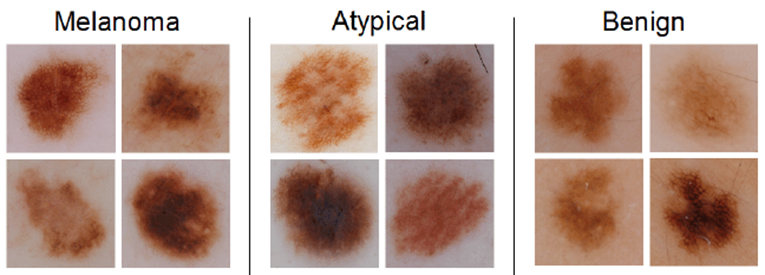
\includegraphics[scale = 0.5]{imagenes/Ejemplo2020.png}
	\caption{Ejemplo de imágenes de ISIC 2017 [23]}
	\label{fig:enter-label}
\end{figure}

\subsubsection{ASAN Dataset}

ASAN (Seung Seog Han 2018)[15][18][19] es un conjunto de datos de origen surcoreano compuesto por lesiones malignas y benignas de la piel. Nos permite obtener un mayor grado de variedad de las imágenes, ya que el repositorio ISIC se centra sobre todo en lesiones de piel de población europea. 

\begin{table}[H]
	\centering
	\begin{tabular}{|c|c|}
		\hline
		\textbf{Tipo de lesión} & \textbf{Número de ejemplares} \\ \hline
		{Actinic keratoses and intraepithelial carcinoma (AKIEC)} & 651 \\ \hline
		{Basal Cell Carcinoma (BCC)} & 1082 \\ \hline
		{Dermatofibroma (DF)} & 1247 \\ \hline
		{Hereditary angioedema (HAO)} & 2715 \\ \hline
		{Intraepithelial Carcinoma (IC)} & 918 \\ \hline
		{Lentigo (LEN)} & 1193 \\ \hline
		{Melanoma (ML)} & 599 \\ \hline
		{Nevus (NV)} & 2706 \\ \hline
		{Pyogenic Granuloma (PG)}  & 375 \\ \hline
		{Squamous Cell Carcinoma (SCC)} & 1231 \\ \hline
		{Seborrhoeic Keratosis (SK)}  & 1423 \\ \hline
		{Wart} & 2985 \\ \hline
		\textbf{Total} & \textbf{17125} \\ \hline
	\end{tabular}
	\caption{Distribución de clases de ASAN dataset}
\end{table}

Tal y como se describe en [17] (M Goyal 2019), este dataset tiene 12 tipos de enfermedades, sumando un total de 17125 imágenes clínicas. Estas imágenes están compuestas en su mayoría por imágenes en miniatura, pero existe un repositorio con imágenes de mayor tamaño, donde sería necesario realizar tareas de segmentación- Sin embargo, dichas imágenes son de acceso restringido, y se requieren permisos especiales del hospital para acceder a ellos. Por ese motivo, tendremos únicamente en cuenta loas 17125 miniaturas.

Adicionalmente, podemos encontrar también imágenes proporcionadas por Hallym, un dataset complementario de 125 imágenes pertenecientes a lesiones de tipo melanoma cancerosas.

Las clases más destacadas de este dataset en su conjunto son la presencia de lesiones benignas de la piel, detalle que no encontramos en ISIC, y que permiten así contrastar información de la piel con lesiones benignas con la piel cancerosa. Podemos encontrar 4 clases benignas: lentigos (manchas solares fruto del envejecimiento y la exposición prolongada al sol), nevus (lunares comunes), verrugas y granulomas benignos. 

\begin{figure}[H]
	\centering
	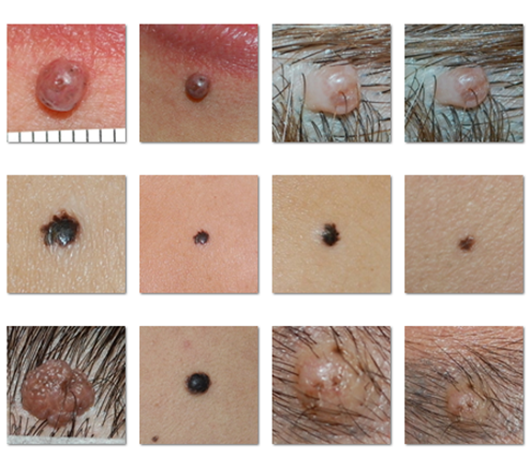
\includegraphics[scale = 0.6]{imagenes/ASAN.png}
	\caption{Ejemplo de lunares beningnos en ASAN (Nevus)}
\end{figure}

Los resultados han sido confirmados por expertos dermatólogos y los resultados verificados en su mayoría mediante biopsia, por lo que las etiquetas asociadas a cada lesión están completamente verificadas.\\

El formato de las imágenes es una disposición matricial de las miniaturas, donde cada fichero que contiene las subimágenes representa en su conjunto una clase. Por desgracia, no se aporta otro tipo de información adicional más allá de la etiqueta por motivos de privacidad.

\subsubsection{Dermnetz}

Podemos encontrar extraer este dataset de un atlas online de enfermedades cutáneas recogidas de pacientes alrededor de todo el mundo. Contiene tanto lesiones benignas como malignas, existiendo además manchas y lesiones vinculadas a enfermedades infecciosas y hongos. 

Existen gran cantidad de herramientas para realizar esta extracción de datos, como la que podemos encontrar en [21]. En total, se pueden obtener hasta 23000 imágenes, existiendo un total de 23 clases no balanceadas. Podemos encontrar lesiones de tipo alérgico, así como acné, dermatitis severa o celulitis.

Carece de metadatos asociados, ya que dicha información es de carácter reservado por su mantenedor.  El dataset no se encuentra listo para usar de forma inmediata, ya que desde 2019, las imágenes deben ser extraídas de la propia web, pues dispone un índice donde se pueden acceder a las enfermedades de interés. El fichero contenedor del dataset fue retirado en 2019 del libre acceso, junto a sus metadatos. Es necesario solicitar su acceso y aportar una cantidad económica.


\subsubsection{ PH2}
El conjunto de datos PH2 [22] es un conjunto de 200 imágenes obtenidas gracias al hospital Pedro Hispano de Portugal. Está compuesto por imágenes de alta resolución que contienen 3 posibles casos de lesiones:
\begin{itemize}
	\item Lunar común (Common Nevus), 80 ejemplares
	\item Lunar atípico (Atypical Nevus), 80 ejemplares
	\item Melanomas, 40 ejemplares.
\end{itemize}

Además de las 200 imágenes, podemos encontrar metadatos asociados a cada una de ellas, como el color, su extensión, textura, forma del borde, localización, entre otros.
Su acceso es libre para fines académicos desde su página oficial [22], que contiene las imágenes en formato jpg, y varios ficheros .csv con la información de la imagen y su clasificación.

\begin{figure}[H]
	\centering
	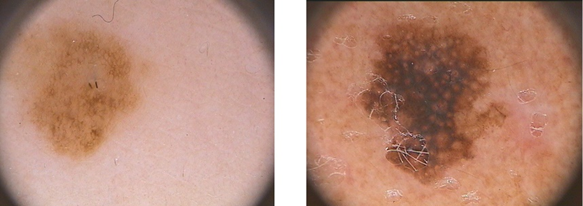
\includegraphics[scale = 0.6]{imagenes/PH2.png}
	\caption{Nevus maligno y benigno en PH2}
\end{figure}

\subsubsection{PAD-UFES 20}

PAD-UFES-20 [25] se trata de un conjunto de datos recopilado de diferentes poblaciones, que contiene diagnósticos para 1.641 lesiones cutáneas únicas recopiladas, comprendiendo un total de 2.298 imágenes.\\

Entre sus clases, podemos encontrar tres enfermedades y tres cánceres de piel.  Todos estos datos han sido recogidos y verificados mediante biopsia en un 100\% de los casos cancerosos, por lo que su diagnóstico está totalmente verificado.\\

Podemos encontrar, además del diagnóstico, metadatos acerca de:
\begin{itemize}
	\item ID de paciente
	\item ID de lesión, 
	\item ID de imagen
	\item Si la lesión benigna fue o no probada por biopsia.
	\item Información del paciente: fumador o no, localización de la lesión, edad, exposición a químicos, historial cancerígeno, etc.
\end{itemize}
Los datos han sido recogidos mediante teléfonos móviles en formato PNG, siendo las imágenes validadas por el Hospital Pathological Anatomy Unit of the University Hospital Cassiano Antȳnio Moraes (HUCAM) de la Federal University of Espírito Santo (Brasil). 
En su publicación original [25], podemos encontrar un resumen de su contenido de forma más específica:

\begin{table}[!ht]
	\centering
	\begin{tabular}{|c|c|c|}
		\hline
		\textbf{Diagnostico} & \textbf{Ejemplares} & \textbf{\% biopsied} \\ \hline
		Actinic Keratosis (ACK) & 730 & 24.4\% \\ \hline
		Basal Cell Carcinoma of skin (BCC) & 845 & 100\% \\ \hline
		Malignant Melanoma (MEL) & 52 & 100\% \\ \hline
		Melanocytic Nevus of Skin (NEV) & 244 & 24.6\% \\ \hline
		Squamous Cell Carcinoma (SCC) & 192 & 100\% \\ \hline
		\textbf{Total} & \textbf{2298} & \textbf{58.4\%} \\ \hline
	\end{tabular}
	\caption{Tabla de casos diagnosticados en PAD-UFES20}
\end{table}

Donde podemos apreciar que todos los casos de enfermedades cancerígenas han sido probados mediante biopsia, y el cáncer de célula basal se trata del tipo de enfermedad más frecuente.

\begin{figure}[H]
	\centering
	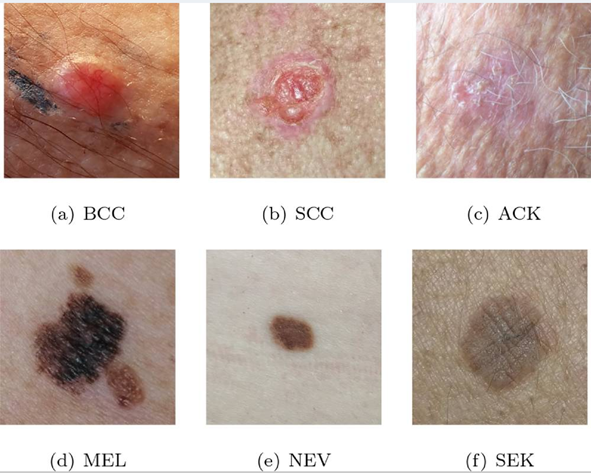
\includegraphics[scale = 0.45]{imagenes/PAD-UFES.png}
	\caption{Batch de ejemplo de PAD-UFES 20 [25]}
\end{figure}

\subsubsection{Severance}
Se trata de un conjunto de imágenes de lesiones cutáneas [24] recopiladas de pacientes de Corea del Sur. Recibe dicho nombre a que los datos recopilados cuentan con la colaboración del Hospital Severance, en el mismo país. \\

En su variante A, que es la única disponible públicamente, podemos encontrar el diagnóstico y otra información asociada sobre 10426 imágenes, cuya valoración se encuentra entre las 38 posibles clases que contiene este conjunto de datos. \\

Seleccionando las 6 clases más comunes contenidas en este dataset, encontraremos que comprenden aproximadamente el 75\% del conjunto. Está compuesto por actinickeratosis (22.5\%), angiofibromas (14.4\%), angiokeratomas(13.8\%), cáncer de tipo basal cell (8.1\%), Becker nevus (7.5\%), bluenevus (6.2\%), y la enfermedad de Bowen (carcinomas)(6.1\%).

El interés en este dataset se debe a que algunas de estas clases mayoritarias, como los nevus azules y de Becker, son condiciones benignas que suelen ser retirados únicamente con fines estéticos, permitiendo complementar con el resto de los diagnósticos negativos. Este tipo de lunares son los más complejos de diagnosticar, debido a sus colores similares a un melanoma, y suelen requerir una biopsia, por lo que su diagnóstico suele alargarse.

Las imágenes se encuentran en formato matriz, por lo que es necesario proceder a su separación previo a su utilización con fines de Deep Learning: 

\begin{figure}[H]
	\centering
	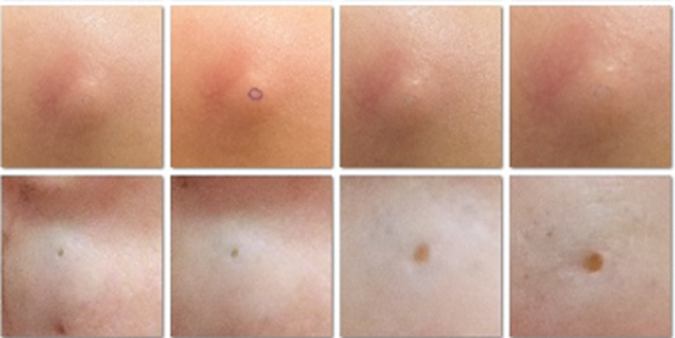
\includegraphics[scale = 0.5]{imagenes/Severance.png}
	\caption{Imágenes de ejemplo provenientes del dataset Severance   }
\end{figure}

\subsubsection{Otros datasets}
Existen otros datasets ampliamente referenciados que son de acceso público. Sin embargo, en los últimos años, éstos han sido retirados y han quedado inaccesibles. Es el caso de DermQuest, un atlas virtual que contenía lesiones cutáneas y otras patologías. Ese dataset fue contenido posteriormente por Derm101, pero ambas versiones fueron retiradas para su descarga. Alternativamente, podemos encontrar algunas de sus imágenes en los datasets SD-198 y SD-260 [26][29], pero únicamente permanece en activo el primero de ellos, bajo solicitud. En total, SD-198 contiene más de 6500 imágenes, mientras que SD-260 alcanzaba las 20000 imágenes.

En el estado del arte actual, podemos encontrar otros datasets ampliamente utilizados, como el caso de DermIS [27], un atlas online de patologías de la piel. También existen publicaciones reciente sobre nuevos conjuntos de datos utilizados de uso restringido, que permiten observar que la tendencia de investigación de este campo sigue en alza; es el caso del estudio propuesto por Papadakis et Al (2021) [28], que recoge datos sobre pacientes con melanoma de grado 3 para estudiar su evolución durante un período de 3 años, para estimar su crecimiento y potencial grosor del tumor.

Debido a las restricciones de acceso, ninguno de estos datasets será empleado como parte del entrenamiento del modelo diseñado para este estudio.

\subsubsection{Conjunto resultado}
Una vez examinados todos los conjuntos mencionados anteriormente, podemos llevar a cabo la unión de todos los datos en un único subconjunto. Esto nos permitirá conseguir un dataset completo y variado con diferentes tipos de piel y diferentes lesiones que nos permitirán identificar multitud de tipos de patologías, siendo posible ajustar el grado de granularidad en función de la agrupación o no de posibles subclases.

Inicialmente, el conjunto de datos construido contendrá todos los subtipos de lesiones cutáneas vistos, pero dispondrán de una segunda etiqueta que indicará si se trata de un caso canceroso o no, atendiendo a su subclase que lo etiqueta. Si agrupamos por lesiones benignas, cancerosas, y potencialmente cancerosas, obtenemos:


\begin{figure}[H]
	\centering
	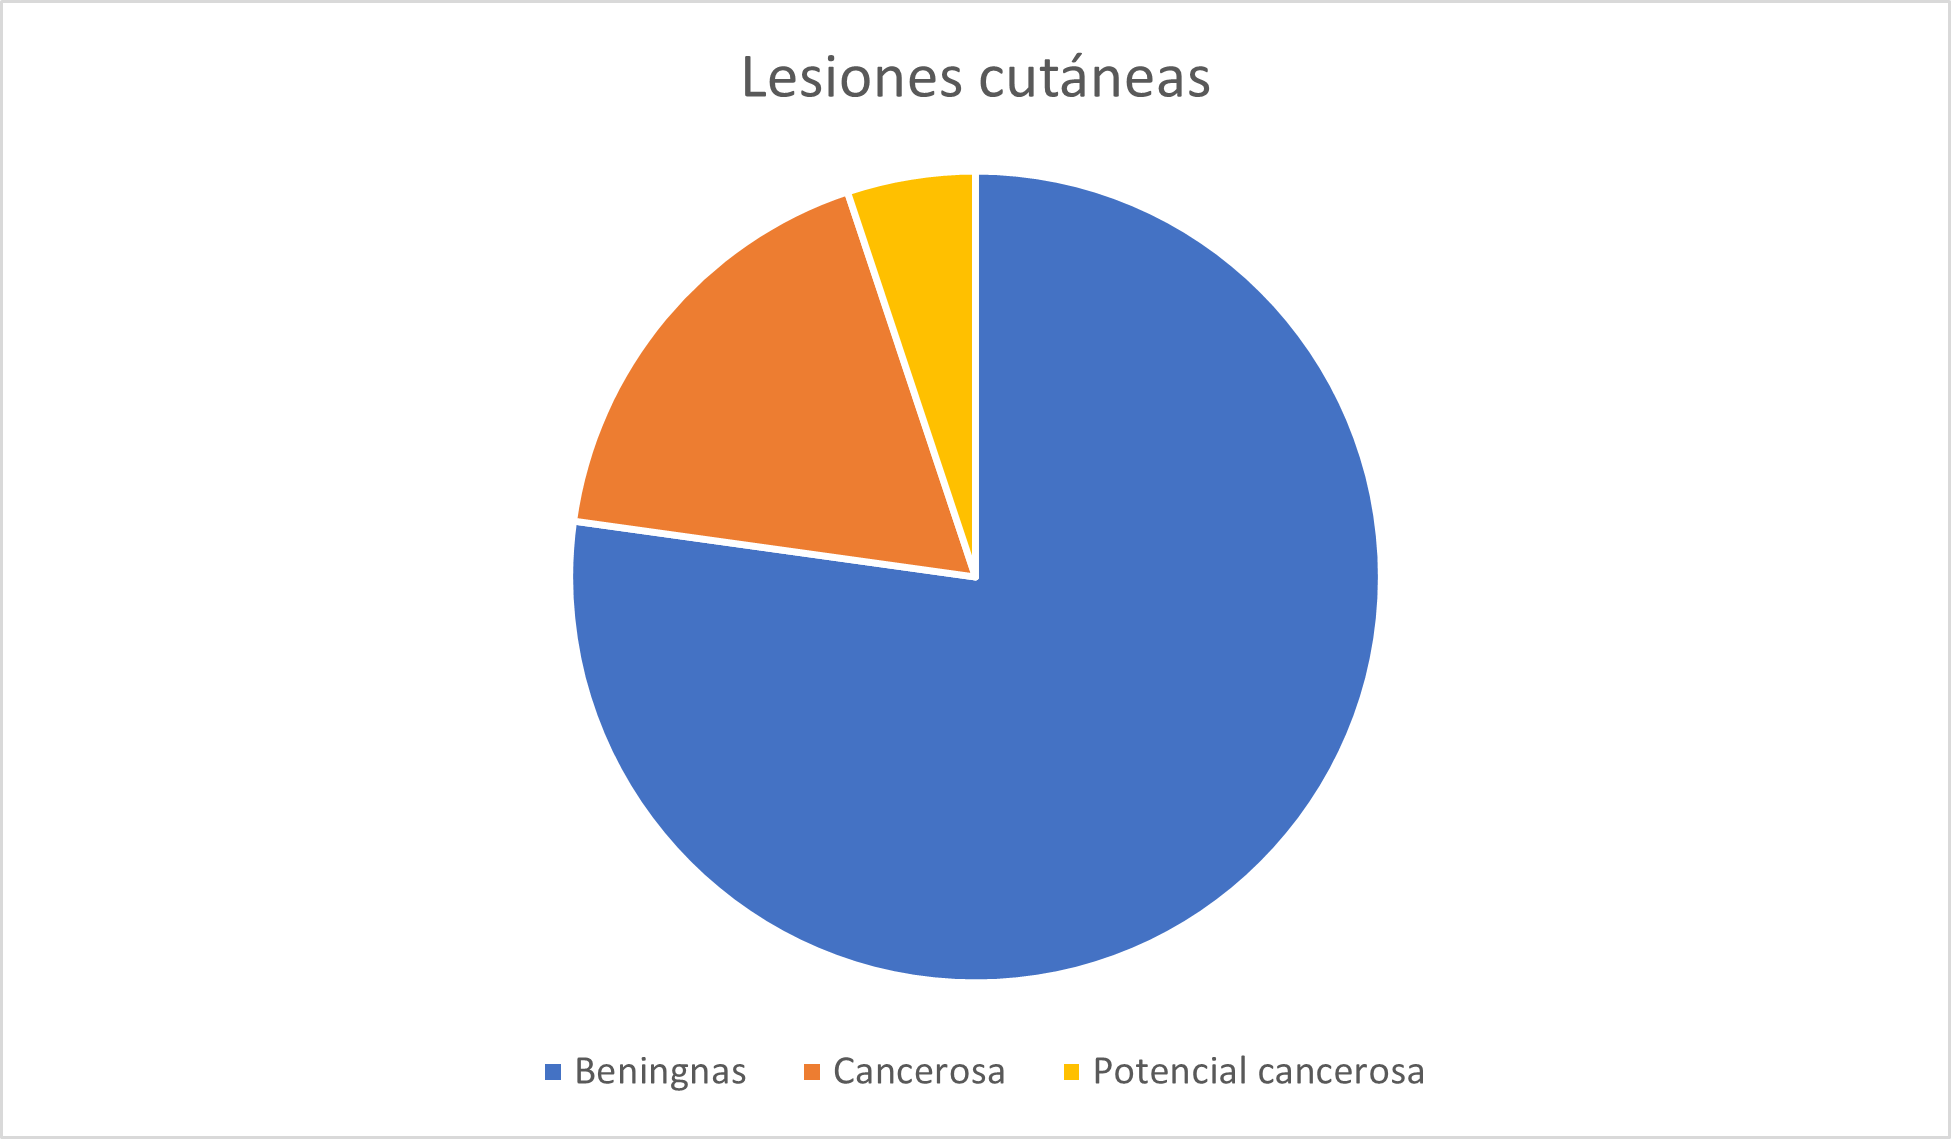
\includegraphics[scale = 0.65]{imagenes/datasetfinal.png}
	\caption{Distribución de clases}
\end{figure}

Se puede observar cómo la mayoría de imágenes disponibles engloban problemas de piel no cancerosos, mientras que el segundo tipo más común de lesión si es la cancerosa. Si atendemos a clasificar las subclases de cada tipo de patología, encontramos 52 posibles etiquetas.

%\section{Procesado de imágenes cutáneas}
%\subsection{Técnicas de reducción de ruido}
%\subsection{Normalización}
%\subsection{Extracción de características}



	
	\chapter{Preprocesado de datos}


Una vez examinados todos los conjuntos mencionados anteriormente, podemos llevar a cabo la unión de todos los datos en un único subconjunto. Esto nos permitirá conseguir un dataset completo y variado con diferentes tipos de piel y diferentes lesiones que nos permitirán identificar multitud de tipos de patologías, siendo posible ajustar el grado de granularidad en función de la agrupación o no de posibles subclases.

Inicialmente, el conjunto de datos construido contendrá todos los subtipos de lesiones cutáneas vistos, pero dispondrán de una segunda etiqueta que indicará si se trata de un caso canceroso o no, atendiendo a la enfermedad que lo etiqueta. En total, tenemos como subclases 52 posibles etiquetas, las cuales iremos examinando a medida que se preprocese cada uno de los subconjuntos.

En el caso de las lesiones potencialmente cancerosas, como se trata de condiciones de la piel no cancerosas con posible evolución a cancerosas, se tendrán en cuenta como imágenes benignas, ya que la condición de malignidad sólo podría aparecer en el futuro, el cual sigue siendo desconocido.

Este proceso es una fase muy delicada del entrenamiento, ya que se ha demostrado empíricamente que una correcta preparación y normalización de los datos permiten hallar soluciones más cercanas a la optima que con datos no procesados. Es importante tener en cuenta que no existe una metodología de preprocesado única, y que es necesario adaptarse al tipo de dato que estamos tratando. Para este proyecto, además, existe una dificultad adicional, y es la existencia de diferentes procedencias para los datos, pues en total se dispone de 5 datasets distintos, cada uno recopilado con diferentes metodologías e instrumentación. Por tanto, será clave adaptarse a cada uno de los destinos, y realizar la partición final de forma estratificada para evitar sesgos que perturben el resutado.

A continuación, se describe la estrategia seguida para el procesado global de los datos, y los ajustes necesarios para cada uno de los conjuntos empleados.

\section{Estrategia de preprocesado para la fusión}

En el punto de partida, antes del preprocesado, contamos con 5 datasets muy diferentes entre sí. Cada uno ha sido documentado y organizado siguiendo unos criterios no estándares que nos afectan en gran medida a la hora de emplear estos datos para el aprendizaje. Antes de proceder con el desarrollo de los modelos, debemos de estadarizarlos a un formato común para evitar que existan clases con el mismo diagnóstico que, por cuestiones de formato, se consideren etiquetadas como clases distintas, por usar criterios distintos de escritura, como ausencia de espacio, mayúsculas o one hot encoding. 

Concretamente, los datos recopilados poseen el siguiente formato de etiquetado:
\begin{itemize}
	\item ISIC: etiquetas escritas a formato completo, como nombre de carpeta, con la primera letra de la enfermedad en mayúscula.
	\item ASAN: nombres escritos en el nombre de la fotografía, haciendo uso de caracteres especiales, y de abreviaturas.
	\item Severance: etiquetas escritas en la propia imagen, la cuales habrá que etiquetar y organizar manualmente, debido a que su csv está incompleto.
	\item PH2: fichero csv, con diagnósticos en formato one hot encoding. Es decir, una fila de ceros y unos, siendo uno la clase a la que pertenece, y 0, el resto.
	\item PAD UFES 20: fichero csv, con los nombres de diagnóstico escritos en minúsculas, sin espacios.
\end{itemize}

Podemos observar la gran variedad de formatos de registro empleados, y que por tanto, es completamente obligatorio y necesario realizar una transformación para hacerlo homogéneo. En este caso, por decisión propia, he considerado adecuado realizar una transformación de las etiquetas al siguiente formato: Uso únicamente de minúsculas, con ausencia de caracteres especiales, nombres sin abreviaturas, y evitando el uso de espacios, con el uso de la barra baja como carácter sustitutivo. Para la clasificación binaria, se utilizará one hot encoding, denotando como 0 los casos negativos y como unos, los positivos.\\


De esta forma, se obtiene un fichero .csv donde encontrar los valores necesarios para entrenar los modelos. Para poder localizar cada imagen, se mantendrá el arbol de directorios por defecto de cada dataset, y se anotará su directorio en un nuevo fichero .csv, que contendrá las etiquetas estandarizadas y los nombres de los ficheros de imagen con y sin el directorio. En resumen, contará con los campos:

\begin{itemize}
	\item image: nombre la imagen, sin el path en su nombre, y con la extensión de formato
	\item dir: directorio donde se aloja la imagen, respetando la estructura de carpetas original seguida por el dataset de origen
	\item label: etiqueta con el diagnóstico de la lesión, siguiendo las pautas indicadas anteriormente
	\item dataset: columna que indica el dataset de procedencia de la imagen, por si fuese necesario utilizar solo un subconjunto de todos los datos.
	\item bin: columna para la etiqueta que indica si se trata de clase Benigna (0) o Maligna (1)
\end{itemize}

\begin{figure}[H]
	\centering
	\label {formatocsv}
	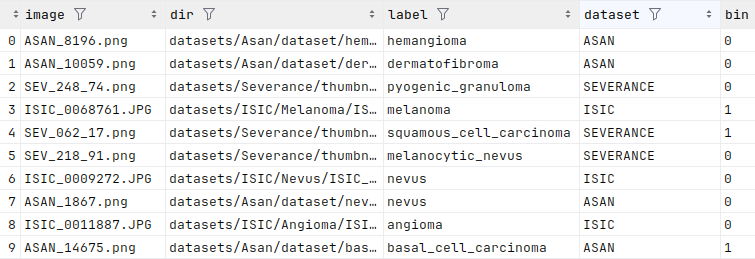
\includegraphics[scale = 0.55]{imagenes/formatocsv.png}
	\caption{Formato del fichero csv normalizado}
\end{figure}

Una vez establecido el formato común, podemos pasar al análisis y adaptación propia de cada conjunto.

\subsection{ISIC Dataset}

El dataset ISIC es el mayoritario de la lista, ya que posee casi 60.000 imágenes de alta resolución, del total de casi 108.000 imágenes de las que disponemos. Para su descarga, se han empleado la galería de la web oficial \cite{isicarchive}, donde podemos filtrar cómodamente las enfermedades que queremos descargar. Como criterio de descarga, se han tenido en cuenta únicamente aquellas fotografías correctamente diagnosticadas, ya que existe un total de 27896 imágenesno etiquetadas dentro del repositiorio, las cuales descartaremos. El problema se centrará en resolver un problema de aprendizaje supervisado, por lo que las imágenes no etiquetadas suponen una complejidad adicional y un ruido para el modelo.

Cada clase descargada, además, se ha sometido a un proceso de filtro, sobre todo por cuestiones numéricas; existen nuevas clases, con escasas cantidades de datos, las cuales poseen menos de 10 imágenes, cantidad insuficiente a la hora de clasificar frente a clases como lunares comunes, que tienen en total 32697 ejemplares. De esta forma, nos queda el siguiente conjunto de clases:
\begin{itemize}
	\item Nevus
	\item Seborreic keratosis            
	 \item Actinic keratosis            
	\item Pigmented benign keratosis         
	\item Solar lentigo                           
	\item Dermatofibroma                          
	\item Vascular lesion                         
	\item LIchenoid keratosis                     
	\item Acrochordon                             
	\item Lentigo NOS                             
	\item Atypical melanocytic proliferation       
	\item Aimp                                     
	\item 	Wart                                     
	\item Angioma                                  
	\item Lentigo simplex                          
	\item 	Neurofibroma                             
	 \item 	Scar 
\end{itemize}

Estas clases se almacenan en ficheros zip cada una, así que tras ser descargadas, deben ser extraídas y añadidas al fichero csv que definimos anteriormente. Al tratarase del primer subconjunto que se añadirá, será la parte del código encargada de crear el fichero y establecer las columnas mencionadas. Además, se realizará la transformación de las etiquetas, dispuestas en el formato de la enumeración anterior, a notación snake case. Numerando el proceso, se ha creado un script de python que realiza las siguientes tareas:

 
 \begin{algorithm}[H]
 	\label{extract}
 	\caption{Algoritmo de descompresión de fotografías por carpetas}
 	\begin{algorithmic}[1]
 		
 		\Procedure{extractISIC}{path}
 		\Comment{Obtener una lista de todos los archivos ZIP}
 		 		\State archivosZip : list of strings
 		 		
 		\ForAll{file in path where file.name endswith('zip')}
 			\State archivosZip.add(file)
 		\EndFor

		\Comment{Iterar sobre cada archivo ZIP}
			\ForAll{archivo in archivosZip}
			\State var rutaArchivoZip  $\gets$ join(path, archivo)
			\State var carpetaSalida = path.splitext(rutaArchivoZip).get(0) \Comment{ Eliminar la extensión}
		
			\If {not exists(carpetaSalida)}
				\State makedir(carpetaSalida) 

			\Comment{  Extraer el contenido del archivo ZIP en la carpeta de salida}
			\State \Call{openZipFile}{rutaArchivoZip} as zipRef
			\State zipRef.extractall(carpetaSalida)
			 \EndIf
		\EndFor
 		\EndProcedure
 		
 	\end{algorithmic}
 \end{algorithm}
 
 


\begin{enumerate}
	\item Extraer las imágenes mediante uzip en una carpeta con el mismo nombre de la clase a la que pertenecen \ref{extract}
	\item Crear un fichero .csv, denominado preprocessedData.csv, donde se alojarán las 5 columnas: images, dir, label, dataset, bin.
	\item Recorrer cada carpeta creada, y añadir los 4 primeros campos
	\item Una vez añadidas todas las imágenes, se renombran las etiquetas a camel case mediante las funciones upper(), lower() y replace() de la clase string de python.
\end{enumerate}

\begin{algorithm}[H]
		 \label{isiccrear}
		\caption{Algoritmo de creación del csv}
		\begin{algorithmic}[1]
			
		\Procedure{crear\_csv}{path, clases, nombre\_dataset}
		\Comment {Inicializa una lista vacía para almacenar la información de los archivos}
		 \State var info\_archivos : list of strings
		 \State i  $\gets$ 0
		
		 \For{nombre\_carpeta in dir(path)}
			\State ruta\_carpeta $\gets$join(path, nombre\_carpeta)
			
			\If{path.isdir(ruta\_carpeta)}
		
				\Comment {Itera sobre cada archivo en la carpeta}
				\For{nombre\_archivo in listdir(ruta\_carpeta)}
						  \State ruta\_archivo $\gets$ join(ruta\_carpeta, nombre\_archivo)
					\If {isfile(ruta\_archivo) and nombre\_archivo.ends() != "jpg"}
						\State var info\_archivos.add(nombre\_archivo, ruta\_archivo, clases[i], nombre\_dataset)
					\EndIf
					\State i = i + 1
				\EndFor
		 	\EndIf
		\EndFor		
		
	
		\State ruta\_archivo\_csv $\gets$ 'preprocessedData.csv'	\Comment{ Define la ruta del CSV}
		
		\State open(ruta\_archivo\_csv) as archivo\_csv
		 \State archivo\_csv.writerow(["image", "dir", "class", "dataset"])  
		 \Comment{Escribe la cabecera}
		 
		 \EndProcedure
	\end{algorithmic}
\end{algorithm}

Para facilitar el procesado, el rellenado de los datos se realiza sobre una estructura tabular de pandas, para así transformar la columna label fácilmente.
En cuanto a la quinta columna, la clase binaria, dicha tarea se realizará cuando todos los datasets estén añadidos al .csv, de forma que el recorrido de los datos sólo se realice una vez, cuando tengamos disponible todas las clases. 

En cuanto al estudio estadístico de los datos, este se realizará una vez dividido los datos en los conjuntos de entrenamiento y test, definido en entradas posteriores.

\subsection{ASAN}

ASAN es uno de los dos datasets cuyo formato de entrega de los datos consistía en una matriz de imágenes en un canvas de gran resolución. En el caso de este dataset, tenemos un total de 32 imágenes de este tipo, cuya etiqueta se encuentra escrita en el nombre del fichero.
El procesado de este dataset será más complejo que el anterior, ya que debemos recortar cada una de las imágenes, evitando que queden bordes blancos que puedan perturbar la predicción, y sesgar el aprendizaje.

Podríamos idear una solución codificada de forma estricta en la cual la imagen se subdivida en n filas y m columnas para extraer las fotografías; sin embargo, cada uno de los canvas del datasets tiene un número filas y columnas concreto que dificultaría esta tarea de forma automática. En su lugar, se ha medido mediante una herramienta de recorte fotográfico el tamaño de una de las miniaturas, siendo este de 98 píxeles, y será el valor que utilizaremos a la hora de realizar el recortado.

No se debe pasar por alto que las imágenes se encuentran separadas vertical y horizontalmente por espacios en blanco, cuya distancia es variable. Es el factor causante de la imposibilidad de partición regular, por lo que se emplearán técnicas de visión mediante la librería OpenCV para la detección de bordes:

\begin{enumerate}
	\item Eliminar 4 píxeles en blanco de los extremos para que todas las bandas blancas queden del mismo grosor
	\item Hallar el numero de imágenes por fila y columana de forma aproximada, teniendo en cuenta el tamaño de miniatura y el borde.
	\item Recortar la imagen usando el método findContours() de openCV. Este método binaria la imagen transformándola a blanco y negro, y trazado con técnicas de detección de puntos de interés en imágenes los bordes de cada una de las miniaturas, y devolviendo las coordenadas de sus equinas en un vector multidimensional. 
	\item Para cada imagen, obtenemos la esquina superior izquierda de la imagen, y mediante el ancho y alto de la imagen, recortamos dicha sección de la imagen y se almacena en una nueva variable.
	\item Se recortan los bordes de dicha imagen y se almacena el resultado en disco, en una carpeta que posee el mismo nombre que la imagen de la que fue extraída.
	\item Se repite el paso 3-6 para cada imagen de la matriz, pasando a abrir la siguiente matriz hasta que no quede ninguna por recortar.
\end{enumerate}

\begin{algorithm}[H]
		\label{cortarasan}
		\caption{Recorte de las imágenes de ASAN mediante OpenCV}
		\begin{algorithmic}
			\Procedure{recortarImagenesASAN}{path, i, title='ASAN'}
			\State var files : list of strings
			
			 \For {f in pathlib.Path().iterdir()}
			 	 \If {f is\_file()]}
			 	 	\State files.add(f)
			 	 \EndIf
			 \EndFor
			 	 
			\State var names : list of strings
			\State var  diss\_class : list of strings
			 \State var i $\gets 0$
			
			\ForEach {f in files}
				   \State name $\gets$ str(f)[str(f).rfind('\#') + 1:-4]
				   \If {f.ends = 'png' and not exists(path)}
						\State {makedir(name)}
						\State var image = cv2.imread(str(f), cv2.IMREAD\_UNCHANGED): image
						\State var gray = cv2.cvtColor(image, cv2.COLOR\_BGR2GRAY) : image
			
						\State var kernel = cv2.getStructuringElement(cv2.MORP H\_RECT, (5, 5))
						\State var gradient = cv2.morphologyEx(gray, cv2.MORPH\_GRADIENT, kernel)
			
						\State var contours $\gets$ cv2.findContours(gradient, cv2.RETR\_EXTERNAL, cv2.CHAIN\_APPROX\_SIMPLE)
			
						\ForEach{cnt in contours}
								\State	x, y, w, h  $\gets$ cv2.boundingRect(cnt)
								\State var box\_image = image[y: y + h, x: x + w] : image
				
								 \Comment{Recorta la imagen para eliminar el borde} 
								\State var img\_sin\_borde = box\_image[grosor\_borde:-grosor\_borde, grosor\_borde:-grosor\_borde]
								\State cv2.imwrite(f"{name}/{title}\_{i}.png", img\_sin\_borde)
					
								\State names.append(f"{title}\_{i}.png")
								\State diss\_class.add(name)
								
								\State i = i + 1
						 \EndFor
				\EndIf	 
	\EndFor
				
\EndProcedure
\end{algorithmic}
\end{algorithm}

Una vez finalizado el proceso, el proceso a aplicar es similar a ISIC; pero, en este caso, en lugar de simplemente convertir a camelcase, debemos de cambiar los nombres por completo para no usar el formato por abreviaturas original, y poder hacer merge de las clases de este dataset con ISIC que sean de la misma enfermedad. Para ello, simplemente se crea un diccionario clave-valor, donde la clave es el nombre que deseamos cambiar, y el valor, el nuevo nombre. Mediante pandas \cite{reback2020pandas}, el proceso de sustitución se puede hacer de forma inmediata mediante la función replace.

Es importante destacar que el dataset Hallym, también será incluido en el conjunto final, siendo el procedimiento de preprocesado a aplicar exactamente el mismo al descrito en este punto.

\subsection{PAD UFES 20}

PAD UFES 20, como ya describimos en el apartado de Estado del arte, se trata de un dataset diseñado para el entramiento de sistemas de asistencia en diagnóstico computado, donde el experto dermatólogo puede utilizarlo como un medio de apoyo. Contiene 6 enfermedades distintas, siendo 3 cancerosas (células basales, células escamosas o melanoma maligno) y 3 benignas (actinic keratosis, nevus, keratosis seborreica).

La estructura de presentación de los datos es más sencilla que ASAN, pues las imágenes son individuales, y cuentan con un fichero .csv donde se describen las etiquetas y otros metadatos asociados a las imágenes. La única modificación necesaria es actualizar el path de cada imagen y la nomenclatura del diagnóstico de la enfermedad, teniendo en cuenta que debemos de tranformar de abreveviatura a camel case:
\begin{itemize}
	\item NEV $\rightarrow$ nevus
	\item SEK  $\rightarrow$ seborreic\_keratosis 
	\item ACK $\rightarrow$ actinic\_keratosis  
	\item BCC $\rightarrow$  basal\_cell\_carcinoma           
	\item SCC $\rightarrow$ squamous\_cell\_carcinoma
	\item MEL $\rightarrow$ melanoma
	         
\end{itemize}



\begin{algorithm}
	\label{cortarpadufes}
	\caption{Formato de las imágenes de PAD UFES}
	\begin{algorithmic}
		\State  var PAD\_UFES\_PATH : directory of PAD UFES 20 dataset
		\State dict $\gets$ \{'BCC': 'basal\_cell\_carcinoma', 'SEK': 'seborreic\_keratosis', 'SCC': 'squamous\_cell\_carcinoma', 'NEV': 'nevus',
			'ACK': 'actinic\_keratosis', 'MEL': 'melanoma'\}
		\Procedure{preparar\_padufes}{}
		\State df\_pad\_ufes $\gets$ file.read()
		\State  df\_pad\_ufes['diagnostic'] $\gets$ df\_pad\_ufes['diagnostic'].replace(dict)
		
		\ForEach{img in df\_pad\_ufes}
			\State df\_pad\_ufes['im\_dir'] $\gets$  PAD\_UFES\_PATH + '/images/ + img
		   \State df\_pad\_ufes['dataset'] = 'PAD\_UFES'
	
	\EndFor		
		\EndProcedure
	\end{algorithmic}
\end{algorithm}

De esta forma, podemos simplemente hacer fusión de las nuevas filas con el fichero anterior en modo de apertura ``append''.

\subsection{PH2}

Este dataset recoge imágenes provenientes del Servicio de Dermatología del Hospital Pedro Hispano (Matosinhos, Portugal), que recoge pruebas cutáneas realizadas con el sistema Tuebinger Mole Analyzer, y un aumento de 20x. Recordando lo analizado en el capítulo anterior, consta de 200 imágenes dermatoscópicas de lesiones melanocíticas, incluidos 80 lunares comunes, 80 nevus atípicos y 40 melanomas, en una resolución de 768x560 píxeles. La base de datos PH² incluye anotaciones médicas de todas las imágenes: segmentación médica de la lesión, diagnóstico clínico e histológico, y evaluación de varios criterios dermatoscópicos. Entre ellos, encontramos distinción por colores; formación del tejido; puntos/glóbulos; rayas; áreas de regresión; velo azul blanquecino (pgimentación difusa).

Los datos se organizan en directorios de carpetas de varios niveles,  pudiendo encontrar en su interior la imagen dermoscópica, la plantilla de segmentación y regiones de interés de la imagen destacadas mediante una plantilla binaria. Para este trabajo, sólo se utilizarán las imágenes correspondientes al directorio de datos dermoscópicos, ya que con debido a la cercanía de la lensión, la imagen contiene en su mayoría solo información útil.

Como preprocesado de las imágenes, al disponer de ellas correctamente clasificadas en carpetas y con un fichero de metadatos bastante completo, el único procedimiento necesario sería la adición al fichero preprocessedData.csv, realizando las conversión a camel case de las labels. El método a emplear es equivalante al utilizado en PAD UFES \ref{cortarpadufes}.

 \subsection{Severance}
 
 Este dataset, como ya se comentó, provinene del hospital Severance, y el dataset con mayor cantidad de patologías identificadas de la lista. El formato de este repositorio sigue una estructura similar a la de ASAN: las imágenes están organizadas en varias páginas de gran tamaño, donde, a diferencia de ASAN, podemos encontrar varias imágenes por lesión separadas entre cuadros blancos, que contienen escritos en él, la etiqueta de las siguientes imágenes leídas de izquierda a derecha, y de arriba a abajo, hasta encontrar el siguiente cuadro en blanco con texto.
 
 La dificultad de este preprocesado radica precisamente en la existencia de los cuadrados blancos, ya que la lectura del texto escrito en ellos es prácticamente imposible. La baja resolución, unido a la existencia de etiquetas cuyo nombre se encuentra dividido en varias líneas, provoca que algoritmos de reconocimiento de texto como Pytesseract \cite {pytesseract} no fuesen capaces de detectar las etiquetas adecuadamente.
 
 Por este motivo, fue necesario identificar manualmente cuántos casos de cada enfermedad existían por matriz de imágenes, y realizar un recuento para saber cuándo aplicar una etiqueta u otra. Conociendo que las etiquetas asignadas aparecían por orden alfabético, el proceso a seguir se resumió en aumentar un contador cada vez que aparecía una imagen en blanco durante el recorrido de las imágenes, y aumentar el contador hasta llegar al valor total de ejemplares de esa clase; en ese momento, se procede a contar los valores de la siguiente. Con este procedimiento, nos queda el algoritmo 3.5(\ref{fig:cortarseverance})
  
La ventaja respecto a ASAN reside en que los espacios en blanco entre imágenes tienen el mismo grosor, y fue posible de separar en submatrices sin necesidad de utilizar ténicas de visión, que ralentizan el proceso extracción. Cada imagen es etiquetada siguiendo el formato establecido  y siendo añadida a una nueva carpeta, desde la cual se referenciarán mediante el fichero preprocessedData.csv. 

Como dificultades a destacar durante el desarrollo de este procedimiento, comentar que la detección de la imagen en blanco que separa las etiquetas entre clases no es trivial. El método elegido para distinguirla es emplear un  umbral de número de píxeles con valor de escala de grises blanco, es decir, 255. El valor de dicho umbral se calculó de forma experimental , ya que si el valor era demasiado bajo, pieles sanas o de color claro también cumplían la restricción. El cambio de etiquetado no se produce si el número de píxeles totales de la imagen encontrada no supera un valor x de miles de píxeles. De forma experimental, el valor 20.000 fue el que mejor resultados aportó, funcionando en todos los casos.

Aumentar de forma desmesurada este valor también puede tener consecuencias negativas, ya que el nombre de la etiqueta se encuentra escrita en la parte inferior de estas imágenes y aportan píxeles de color negro que no cumplirían la condición.


 \begin{algorithm}[H]
	\label{fig:cortarseverance}
	\caption{Recorte de las imágenes de Severance mediante OpenCV}
	\begin{algorithmic}
		\Procedure{recortarImagenesSEVERANCE}{path}
		
		\State  df\_sev $\gets$ read('SeveranceA.xls')
		\If {not os.path.exists('thumbnails')}
		\State makedir('thumbnails')
		\EndIf
		
		\State var files : list of strings
		
		\For {f in pathlib.Path().iterdir()}
		\If {f is\_file()]}
		\State files.add(f)
		\EndIf
		\EndFor
		
		\State var names : list of strings
		\State diss\_class : list of strings
		\State j $\gets 0$
		
		\For {f in files}
		\If {f.ends = 'jpg'}
		\State name $\gets$ f.name[0:-4]
		\State {makedir(name)}
		\State var image = cv2.imread(name, cv2.IMREAD\_UNCHANGED): image
		\State var image\_split = $\begin{matrix}
			[ image_1 image_2, \ldots, image_8 ] \end{matrix}^T$	\Comment{División por filas}
		
		
		\State var i $\gets$ 0
		
		\ForEach{im  in image\_split}
		\Comment{Recorta la imagen en columnas}
		\State image\_split\_col = np.split(im[:, 2:-3], 15, axis=1)
		\ForEach {imcol in image\_split\_col}
		\State img\_sin\_borde$\gets$ imcol[grosor\_borde:-grosor\_borde, grosor\_borde:-grosor\_borde]
		\If {np.count\_nonzero(imcol == 255) > 20000)}  \Comment{Si es imagen de separador con nombre}
		\State j $\gets j + 1$  \Comment {Cambiamos de etiqueta al siguiente paciente}
		\State continue
		\Else
		\State actual  $\gets$ df\_sev.get(j)
		
		\State	actual.add('{name}\_{i}.png')
		\State	trainProcessed.add(actual)
		\Comment{Guardamos la imagen y añadimos su nombre}
		\EndIf
		\State cv2.imwrite(f'thumbnails/{name}\_{i}.png', img\_sin\_borde)
		\State names.append(f"{name}\_{i}.png")
		\State i $\gets i + 1 $
		
		\State diss\_class.add(name)
		\EndFor
		
		\EndFor
		\EndIf	 
		\EndFor
		\State trainProcessedDF.write("severanceTrainingSet\_thumbnails.csv") \Comment{Guardado en disco}
		\EndProcedure
	\end{algorithmic}
\end{algorithm}
 
 \subsection{Etiquetado binario}
 
Una vez disponemos de todas las imágenes correctamente etiquetadas y redireccionadas desde el fichero preprocessedData.csv, podemos continuar con el etiquetado binario de las enfermedades. Para disponer también de los datos de malignidad de las enfermedades, se ha realizado manualmente una distinción de las distintas enfermedades entre benignas y malignas. Debido a la minoría de imágenes por defecto, para reducir el tamaño del diccionario de enfermedades, por defecto se establecieron todas las etiquetas por defecto a 0, y aquellas pertenecientes al subconjunto de malignas, a 1, siguiendo el siguiente procedimiento:
 
 \begin{enumerate}
 	\item Crear una nueva columna, de nombre ``bin'', que contendrá 0 como valor de inicialización.
 	\item Construir un diccionario o lista con aquellas enfermedades que son malignas.
 	\item Se recorre la columna target para comparar la enfermedad del ejemplar con la lista de enfermedades malignas. En caso de ubicarse en ella, se cambia el valor de ``bin'' por un 1.i
\end{enumerate}

De esta forma, obtenemos la quinta columna, expresada con ceros y unos. Dependiendo de la función de pérdida y el framework posteriormente utilizado, estas etiquetas tendrán que ser categóricas, pero dicho paso puede realizarse de forma inmediante con un casting de tipos, o bien, un el uso de la función replace de python ya mostrada en la fase de homogeneización de los datos.



\begin{figure}[H]
	\centering
	\label {tartabinaria}
	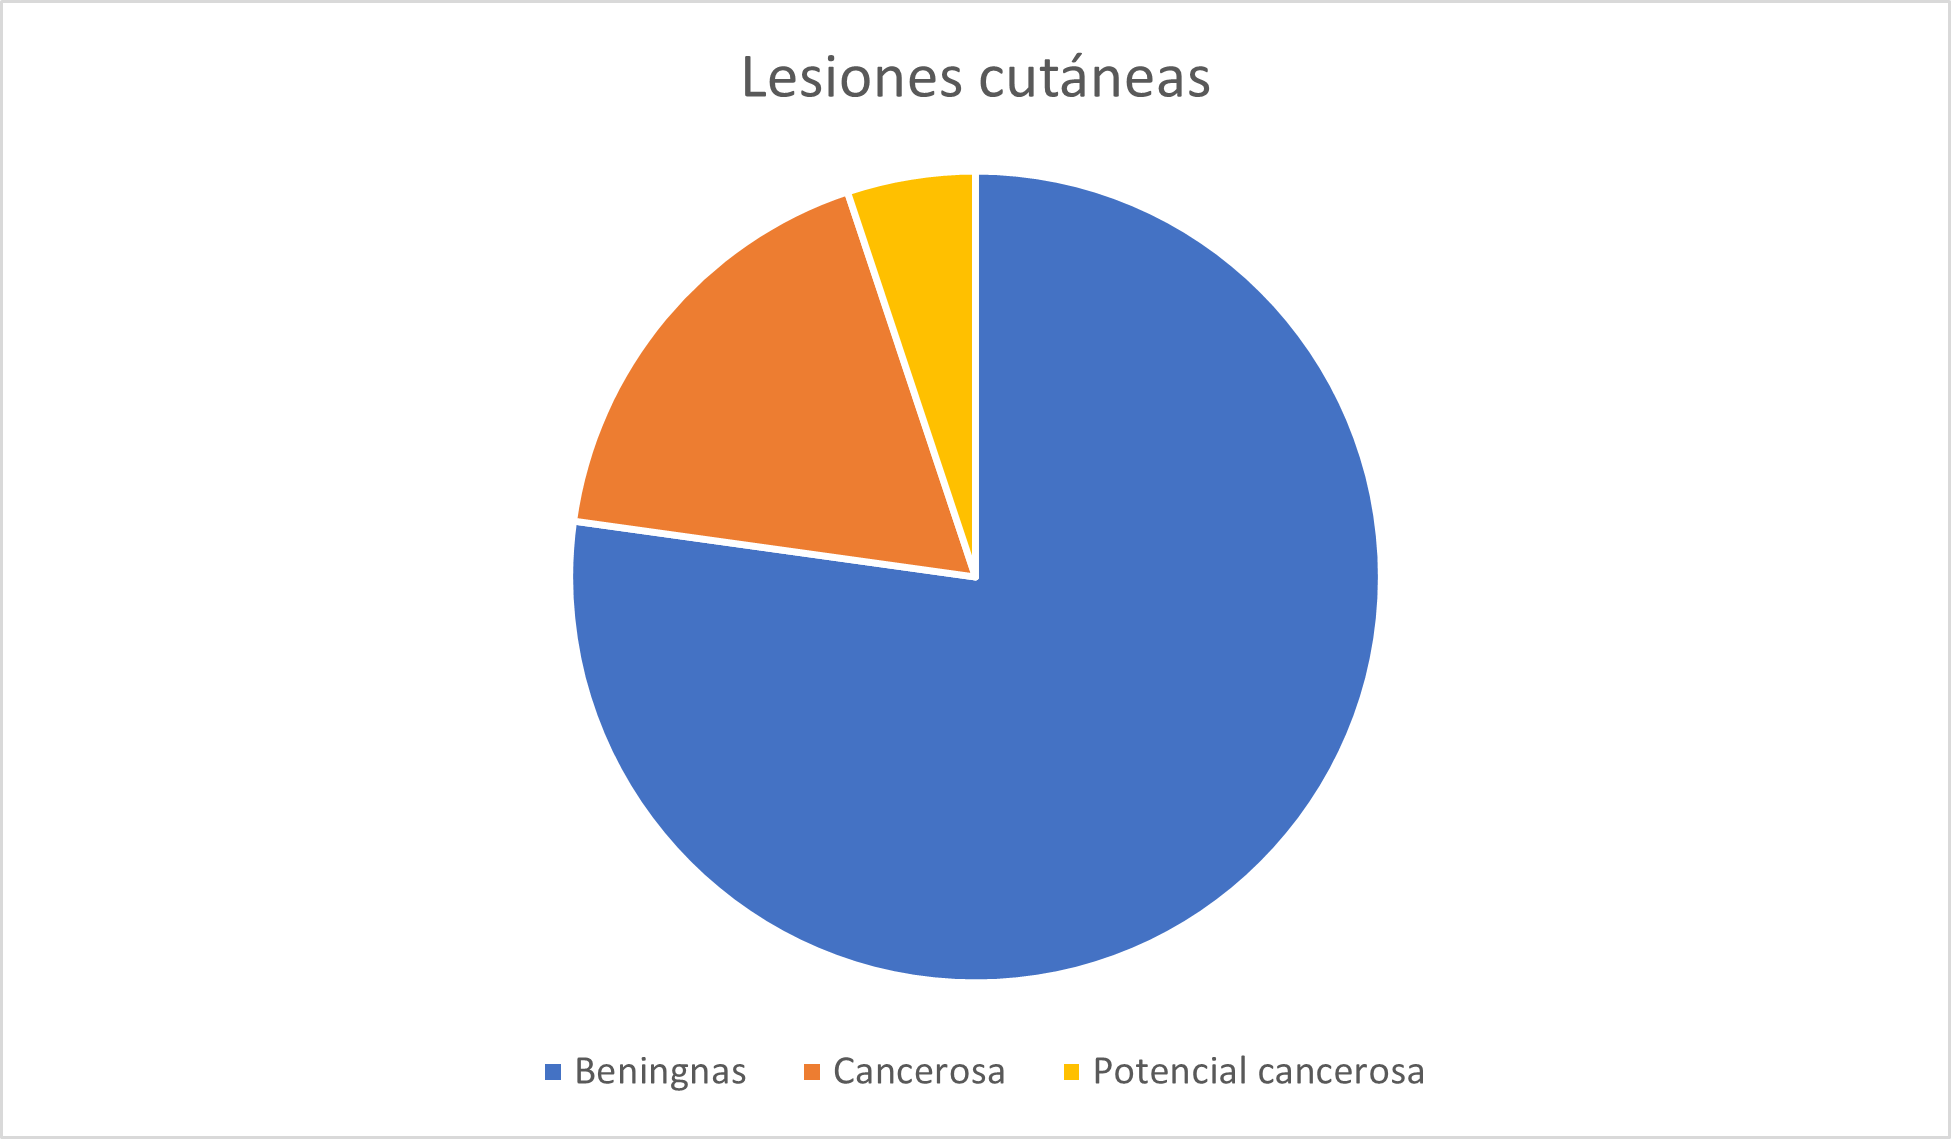
\includegraphics[scale = 0.7]{imagenes/datasetfinal.png}
	\caption{Distribución de clases}
\end{figure}

Si agrupamos por lesiones benignas, cancerosas, y potencialmente cancerosas, podemos obtener el siguiente diagrama de sectores de la figura \ref{tartabinaria}, donde se puede observar cómo la mayoría de imágenes disponibles engloban problemas de piel no cancerosos, mientras que el segundo tipo más común de lesión si es la cancerosa. Las lesiones potenciales, como ya se comentó, pasan a formar parte de las lesiones benignas debido a que en el momento de la captura, continúan siendo benignas.

Con este paso, finalizamos la uniformización de los datos en lo que corresponde al formato del etiquetado y gestión de directorios. A continuación, se realizarán las fases de partición de los datos, y de preprocesado de la imagen en sí, empleando como referencia el estudio realizado en el estado del arte.


\section{Particionado de los datos}

En este punto, estudiaremos la importancia de un correcto particionado de los datos para el entrenamiento del modelo y su posterior verificación de rendimiento. Se estudiará la importancia de disponer de un estimador insesgado del modelo entrenado, y las decisiones tomadas para el problema que nos concierne.

\subsection{Importancia de la separación train-test}
En las tareas de aprendizaje de Machine learning y Deep learning, el objetivo es disponer del mayor número de datos posible, por lo que la opción de privar al proceso de entrenamiento de un subconjunto de ellos, o incluso proceder a su eliminación, puede ser una decisión demasiado drástica que ha de tomarse con fundamento.\\

Sin embargo, cuando realizamos un modelo de aprendizaje, realmente estamos creando una hipótesis, un modelo que construimos y queremos hacer que se acerque lo máximo posible a la expresión que define la población real del problema. Pero, para poder estimar la bondad de nuestro ajuste de forma fiable, necesitamos algún estimador no sesgado que nos indique la calidad del modelo, que nos permita saber el error que comete nuestra hipótesis con respecto a la distribución de la población real, al que denominaremos como error fuera de la muestra, abreviado como $E_{out}$.  Esto se debe a que, para construir este modelo aproximado, estamos empleando una muestra de la población, la cual es continuamente iterada para ir ajustando los filtros aplicados sobre el conjunto y que permite inferior de sus características extraídas las etiqueta de cada una de las imágenes.\\

Podemos conseguir un estimador insesgado separando un conjunto de datos del total, y obteniendo un conjunto de test, el cual no se ha visto involucrado en ninguna fase del proceso de aprendizaje. La hipótesis final, a la que llamaremos $g$, es evaluada en este subdataset, y el resultado será un buen estimador del $E_{out}$. A este error podemos llamarlo $E_{test}$. Al seleccionarlo como estimador de $E_{out}$, estamos afirmando de alguna manera de que éste se tratará de un estimador que generaliza muy bien el error out-of-sample.\\

Este conjunto recibirá un número efectivo de hipótesis $|\mathcal H|= 1$, es decir, únicamente es evaluado con la hipótesis final de nuestro modelo (su ajuste paramétrico final). Esta hipótesis se elige sin conocer el comportamiento de los datos que el conjunto de test contiene, ya que si la estimación de $g$ se ve afectada de alguna forma por los ejemplares ya utilizados en el entrenamiento, no conseguiremos un estimador insesgado, y la ecuación de Hoeffding, no será aplicable. Dicha ecuación enuncia, que para muestras idénticamente distribuidas, e independientes entre sí, se cumple la siguiente desigualdad \cite{Mostafa2012}:

$$P(\mathcal{D}: | E_{out}(h) E_{in}(h) |  > \epsilon \leq 2e^{-2\epsilon^2	N}$$

Donde, para cualquier valor de $\epsilon$:
\begin{itemize}
	\item $\mathcal{D}$ es el nombre que recibe el conjunto de entrenamiento.
	\item $ E_{out}$ es el error out-of-sample, error teórico con respecto a distribución real de los datos.
	\item  $E_{in}$ es el error in-sample, es decir, el error cometido durante el proceso de entrenamiento entre las etiquetas inferidas, y su valor real, también conocido como y verdadero.
	\item $N$ es el tamaño de la muestra de datos disponible.
\end{itemize}

Es decir, se cumple que $E_{out}$ se convierte en un estimador muy cercano al valor real del modelo. Dichas restricciones de independencia y pertenencia a la misma distribución son claves,
 motivo por el cual la eliminación de imágenes duplicadas fue clave (ya que cualquier contaminación entre el conjunto de entrenamiento y aprendizaje puede crear sesgos al alza en los resultados). \\

El valor del entrenamiento $E_{in}$ sí que sería un estimador sesgado de forma optimista, pues el modelo ha adaptado los filtros para ser capaz de inferior el mayor número posible de etiquetas correctas del conjunto de entrenamiento.. Pero esto no ha ocurrido con test, por lo que podemos dar como resultado un estimador fiable y robusto de cómo se comportará nuestro modelo con otros elementos de la población real.\\

Cuanto mayor es el tamaño del conjunto, más cercano será el valor del error de nuestra partición de test, $E_{test}$, con respecto a $E_{out}$. Pero, cuantos menos datos para entrenar dispongamos, menos se parecerá la estimación al comportamiento real de la población, y a $f$. Tenemos que conseguir un equilibrio entre ambos tamaños para aprovechar la mayor cantidad de datos posibles, pero disponiendo de un $E_{test}$ fiable. Normalmente, los valores recomendados suelen ser entre un 10\%-30\% de porcentaje de los datos dedicados al conjunto de test, quedando entre un 70-90\% de datos de entrenamiento. Para este problema, la separación entrenamiento-test elegida ha sido 60-40, respectivamente, que a priori, puede ser muy elevada y salir de la recomendación empírica, pero debido a la existencia de grandes desiquilibrios y una cantidad de datos más que suficiente, de aproximadamente 110.000 ejemplares, podemos obtener de esta forma un estimador muy fiable.\\

A continuación, se realizará todo el proceso de separación de datos, entre entrenamiento y test en proporción 60-40. Aunque, idealmente, este proceso de hace de forma completamente aleatoria y sin intervención, he optado por realizar la separación de forma estratificada. Esto hace referencia al mecanismo de separación de los datos teniendo en cuenta el conteo de cada una de las clases. Lo que he realizado ha sido, en primer lugar organizar los datos por sus respectivas clases, dentro de cada dataset, de forma que se tienen dos vectores cuyo contenido son las tuplas de cada clase por separado. 

Pero este aspecto no solo se da a nivel de subdataset, sino también a nivel del dataset global; es importante tomar una cantidad proporcional de cada clase para evitar que el algoritmo sesgue sus resultados al encontrar patrones comunes propios de cada subconjunto, y este no sea capaz de aprender la visión general de los elementos que definen a un tipo de lesión concreto. Por tanto, definiré un ``doble nivel de estratificación'', donde:

\begin{enumerate}
	\item A nivel de cada subdataset, extraer mediante partición estratificada un porcentaje de entrenamiento, y otro de test en proporción 60-40 a la hora entrenar.
	\item Volver a unir las clases de entrenamiento de cada dataset, y test de cada dataset, en los dos ficheros que comprenderán las imágenes asociadas al conjunto de entrenamiento y al conjunto de test.
\end {enumerate}

De esta forma, podemos conseguir proporcionalidad entre dataset y entre clases entre train y test, y hacer que la distribución de las imágenes sea prácticamente la misma. Aunque normalmente se suele realizar la separación de forma completamente aleatoria, en clasificación podría darse el caso extremo en el que una clase completa no aparezca en el conjunto de entrenamiento, y nuestro modelo obtenga pésimos resultados de $E_{test}$.  Si bien la probabilidad es muy baja, matemáticamente puede ocurrir, y considero que no afecta negativamente al análisis haber realizado la partición de forma proporcional a cada clase y dataset.

Comentando en detalle la implementación realizada, es de interés destacar el empleo de la función train-test split de SKlearn \cite{scikit-learn}. Se trata de una función que realiza de forma bastante simplificada el proceso de partición estratificada. En este caso, además, se verificará la existencia de clase con menos de 16 ejemplares de imagen presentes para confirmar que no se han filtrado clases minoritarias las cuales son imposibles de clasificar con el modelo actual.

El resultado es el siguiente:

 \begin{algorithm}[H]
	\label{fig:separar}
	\caption{ Separación de las filas según el valor de la columna ``column''}
	\begin{algorithmic}
		\State MIN\_COUNT = 16
		\Procedure{separar\_subdata}{dataframe, column}
		\State var separated $\gets$ dataframe $\matrix{[c_1, c_2, \cdots, c_n]} / c_{i _j}= column$ y $separated[k] \cap separated[l] = {0}$ para $k\neq l$
		\State var trainData, testData: list of tuples
		\State lista\_elementos: array of tuples
		
		\ForEach{ data\_part, contenido in separated}
			\State lista\_elementos = lista\_elementos $\cup$ contenido
			\If { lista\_elementos["class"].map(counts) > MIN\_COUNT}
				\State var train, test = \Call{train\_test\_split}{subdata, test\_size=0.4,seed=19, shuffle=True, stratify=subdata['class']}
				\State  trainData = trainData $\cup$ train
				\State  testData = testData $\cup$ test
			\EndIf
		\EndFor \\
	\Return lista\_elementos
		
		\EndProcedure
		
	\end{algorithmic}
\end{algorithm}

De esta forma, seguimos manteniendo la proporción a nivel de conjunto global, y de subdataset. En caso de necesitar entrenar únicamente con uno de los subconjuntos añadidos, podemos filtrar el cojunto de tuplas por aquellos cuya clase sea igual a la buscada.

\subsection{Particionado de validación}
	
	%\chapter{Técnicas de aprendizaje}
	
	%\chapter{Aprendizaje mediante Deep Learning}
	
	%\chapter{Comparativa de modelos y rendimiento}
	
        \chapter{Diseño de la aplicación para el cáncer de piel}

Una vez han sido creados, entrenados y verificados los modelos cuantizados para teléfono móvil, podemos proceder con el diseño e implementación de la aplicación. Su objetivo será, mostrar de forma visual y cómoda para el usuario habitual, la utilidad de los modelos entrenados y optimizados en los capítulos \ref{sec:capt5} y  \ref{sec:capt6}  de este trabajo.

Al tratarse de una aplicación para uso local en el dispositivo, y de funcionalidades concretas y bien delimitadas, como lo es la prueba de los modelos en casos reales, esta no será excesivamente compleja. Aun así, en este capítulo, abordaremos su diseño desde el punto de vista de la ingeniería del software, para detallar correctamente las funcionalidades necesarias y los requisitos que debe cumplir para que el resultado sea el esperado.

\section{Descripción del problema. Requisitos y definiciones.}
\label{sec:descripcion}

Comenzaremos por analizar la descripción de la aplicación que queremos conseguir, teniendo en cuenta los términos relevantes del texto y extrayendo los requisitos a cumplir por la misma.

\subsection{Proceso de obtención de requisitos}

En  primer lugar, se describe el problema a resolver, y los requisitos del mismo.

\subsubsection{Descripción}
Tras el entrenamiento de tres modelos de aprendizaje profundo orientados a la prognosis y el diagnóstico de enfermedades cancerígenas de la piel, es necesario crear una plataforma simple capaz de demostrar al usuario la versatilidad y precisión de los modelos haciendo uso de imágenes que contienen lesiones cutáneas, de manera que los modelos sean capaces de diagnosticar si la imagen se trata de un caso positivo o negativo de una enfermedad cancerígena, y clasificar su posible diagnóstico empleando dichos modelos.

El diagnóstico de imágenes debe realizarse teniendo en cuenta la existencia de un usuario, que puede tomar fotografías de este tipo de lesiones, y que debe recibir el resultado del examen, para que este pueda tomar medidas en caso de tratarse de enfermedades sospechosas y visitar al dermatólogo cuanto antes. Para ello, debe clasificarse, en primer lugar, si se trata de una enfermedad maligna o benigna, y posteriormente, un posible subtipo de enfermedad.

De forma detallada, el proceso sería el siguiente:

\begin{enumerate}
	\item El usuario ingresa en el sistema, y requiere al mismo la realización de un diagnóstico por medio de imagen.
	\item El usuario obtiene la imagen de la enfermedad que desea analizar empleando para ello la cámara del dispositivo, o bien, una fotografía ya realizada en el pasado que desee clasificar.
	\item A continuación, se realiza el diagnóstico empleando dos niveles de análisis: 
	\begin{enumerate}
		\item Primero, se realiza una clasificación más general para identificar si se trata de una enfermedad benigna, o de un tumor maligno.
		\item En función del resultado de la prueba, se procede al empleo de uno de los modelos especializados para identificar el posible tipo de enfermedad que puede ser, atendiendo a los casos más probables a nivel clínico.
	\end{enumerate}
	\item Una vez terminada la aplicación de los modelos de aprendizaje para la clasificación, se asignará de forma definitiva un diagnóstico, que será obtenido en base a los resultados probabilísticos más altos de la salida de los modelos evaluados. Esta información, junto con la miniatura de la imagen, y una descripción de la enfermedad, será mostrada al usuario en pantalla, no tardando más de dos segundos y empleando ventanas flotantes para una mayor legibilidad.
\end{enumerate}

\subsubsection{Objetivos a tener en cuenta}

Para la realización del producto final, han de tenerse en cuenta los siguientes aspectos:

\begin{itemize}

	\item El usuario debe ser capaz de aportar la imagen para el diagnóstico empleando su galería o bien la cámara de su dispositivo. Opcionalmente, puede ofrecerse la posibilidad de rotar o recortar la imagen objetivo.
	\item Se debe incluir información de uso para facilitar al usuario el proceso de aportación de la información.
	\item Se debe tener en cuenta que el cliente no disponga de fotografías existentes, y deba realizar una nueva para continuar el proceso de diagnóstico.
	\item Los diagnósticos realizados deben ser visibles ordenados de mayor a menor antigüedad en una sección dedicada, de forma que el usuario sea capaz de revisitar los casos anteriores y realizar un seguimiento de los mismos.
	\item La implementación se ha de realizar en Java o Kotlin, de manera que la app sea compatible con dispositivos Android.
	\item El sistema ha de tener un comportamiento fluido y dinámico para el usuario, no tardando más de dos segundos por imagen para realizar el diagnóstico.
	\item La interfaz de usuario ha de ser fluida y eficiente, con el menor tiempo de carga posible entre funcionalidades.
	\item El almacenado del histórico ha de realizarse de forma local para velar por la privacidad del usuario.
	\item Los modelos de aprendizaje empleados han de ser compatibles con el estándar TorchScript/PyTorch \cite{paszke2019pytorch}.
\end{itemize}

\subsection{Requisitos}

Una vez analizado el problema, podemos identificar una serie de requisitos que debemos cumplir. Estos pueden clasificarse en tres tipos:

\begin{itemize}
	\item \textbf{Requisitos funcionales}. Describen la interacción entre el sistema y el entorno, indicando como ha de reaccionar la aplicación ante ciertos estímulos.
	\item \textbf{Requisitos no funcionales}. Especifican restricciones del sistema no relacionadas directamente con su comportamiento funcional, pero que son clave durante el diseño e implementación del sistema.
	\item \textbf{Requisitos de información}. Establecen las necesidades de almacenamiento del producto software que se está desarrollando.
\end{itemize}

Podemos encontrar los requisitos siguientes para el problema descrito.

\subsubsection{Requisitos funcionales}

\begin{itemize}
	\item \textbf{RF-1}. El usuario debe ser capaz de realizar el diagnóstico de una fotografía empleando el modelo de inteligencia artificial subyacente. Debe ofrecer al usuario retroalimentación sobre la enfermedad, como su nombre y descripción de la gravedad.
	\begin{itemize}
		\item \textbf{RF-1.1}. El sistema debe proporcionar la funcionalidad al usuario de leer la imagen de galería o mediante nueva fotografía.
		\item \textbf{RF-1.2}. El usuario debe poder recortar la imagen y seleccionar el área de interés.
	\end{itemize}
	\item \textbf{RF-2}. El sistema debe ofrecer la posibilidad al usuario de mostrar el historial de fotografías examinadas. Cada fotografía debe ser correctamente ordenada por su fecha y hora de toma, en orden descendente.
\end{itemize}

\subsubsection{Requisitos no funcionales}
	\begin{itemize}
		\item \textbf{RNF-1}. El tiempo de respuesta del modelo de aprendizaje debe ser inferior a 2 segundos.
		\item \textbf{RNF-2}. El lenguaje de programación a emplear debe ser Java o Kotlin.
		\item \textbf{RNF-3}. La interfaz de usuario ha de ser implementada mediante ficheros XML, y siguiendo los requisitos de diseño de Material Design\footnote{Material Design: \url{https://m3.material.io/}} de Google para cumplir con las especificaciones de interfaz de Android.
		\item \textbf{RNF-4}. La inferencia del modelo de aprendizaje ha de realizarse empleando imágenes tipo bitmap de 512 x 512.
		\item \textbf{RNF-5}. La implementación del proceso de inferencia debe hacer uso de la libería PyTorch mobile y TorchScript.
		\item \textbf{RNF-6}. El recorte de la imagen debe realizarse a tiempo real.
		\item \textbf{RNF-7}. El menú de histórico de diagnósticos ha de ser sencillo, con opción de scroll, e implementado con un ViewPager de Java para poder ordenar los casos de mayor a menor antigüedad.
	\end{itemize}
\subsubsection{Requisitos de información}

\begin{itemize}
	 \item \textbf{RI-1: Historial}. El historial debe almacenar la información de cada diagnóstico realizado en el tiempo. Debe almacenarse de forma local en la memoria secundaria del dispositivo.
	 \begin{itemize}
	 	\item Contenido: imagen miniaturizada del diagnóstico, nombre de la enfermedad diagnosticada y si se trata de una patología benigna o maligna. 
	 	\item Requisitos asociados: RF-4, RF-5, RF-6.
	 \end{itemize}
	\item  \textbf{RI-2: Descripción de las enfermedades}. Almancena un breve resumen para cada enfermedad, codificada por su nombre de etiqueta.
		 \begin{itemize}
		\item Contenido: nombre de la enfermedad, descripción.
		\item Requisitos asociados: RF-4, RF-5, RF-6, RF-7.
	\end{itemize}
\end{itemize}

\subsection{Glosario de términos}
Las palabras clave de la descripción se recopilan en la siguiente lista:
\begin{itemize}
	\item \textbf{Diagnóstico}. Proceso mediante el cual se identifica la enfermedad de un paciente.
	\item \textbf{ Prognosis}. Acción de pronosticar, o juzgar médicamente una condición de un paciente.
	\item  \textbf{Lesión cutánea}.Mancha o tumor de características sospechosas originado en la piel.
	\item  \textbf{Modelo de aprendizaje profundo}. Algoritmos basados habitualmente en el uso de arquitecturas neuronales, empleados para la clasificación o segmentación de imágenes de entrada con el fin de dar como salida una clasificación o característica de relevancia sobre la entrada.
	\item  \textbf{Ventana flotante}. Interfaz de usuario que se superpone de forma total o parcial sobre una ventaja ya existente. En Android, esta funcionalidad es implementada por los fragmentos, o bien, el uso de otros componentes específicos como ventanas de scroll.
\end{itemize}

\section{Modelo casos de uso}

Una vez especificados los requisitos del proyecto software que debemos cumplir, incluyendo las funcionalidades del mismo y las limitaciones técnicas asociadas, podemos proceder a la definición de los casos de uso de nuestro proyecto. Para ello, debemos estudiar los actores presentes en la interacción con el sistema, y aislar las funcionalidades a implementar. En resumen, definiremos el punto de vista de los usuarios de nuestro sistema y el contexto de uso del mismo.

 \subsection{Representación de los casos de uso}
 
 Dentro de la aplicación, podemos identificar, basado en los requisitos anteriores, dos objetivos a satisfacer por el usuario: realizar un diagnóstico (figura \ref{fig:diagcu}), y consultar el historial de pruebas realizadas (figura \ref{fig:histcu}).
 
 \begin{figure}[H]
 	\centering
 	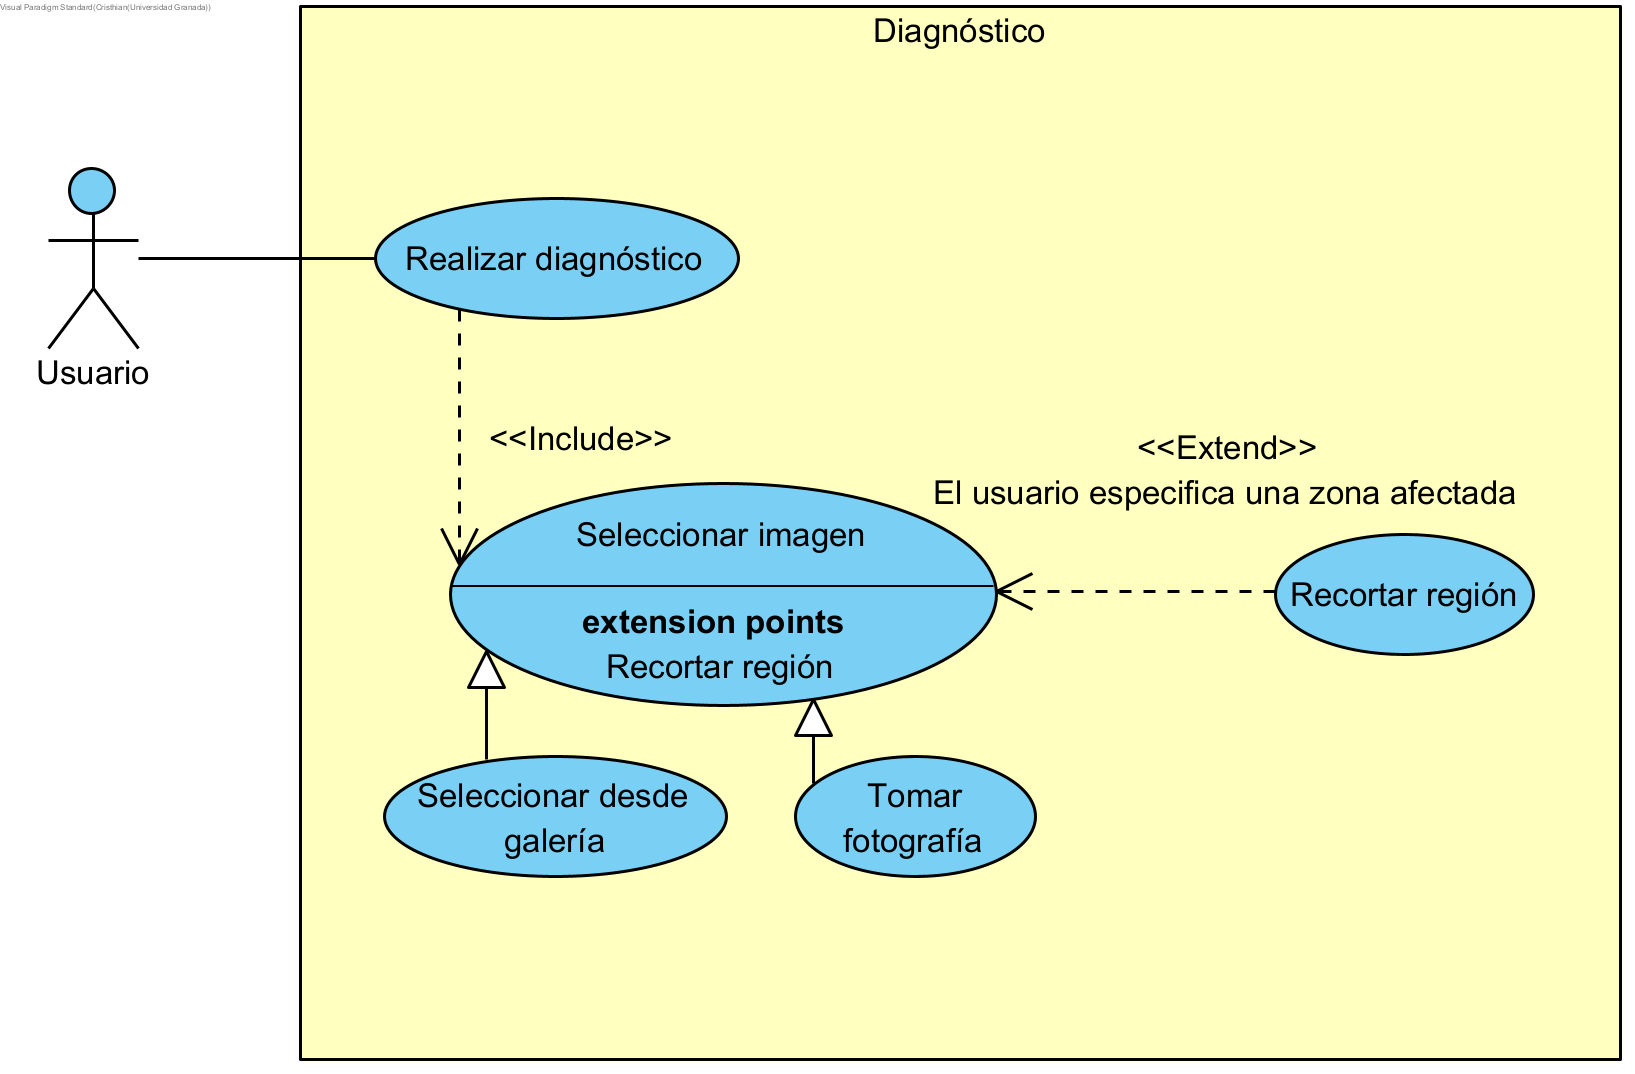
\includegraphics[scale = 0.9]{imagenes/TomarFoto.png}
 	\caption{Caso de uso: Diagnóstico}
 	\label{fig:diagcu}
 \end{figure}
 
 
  \begin{figure}[H]
 	\centering
 	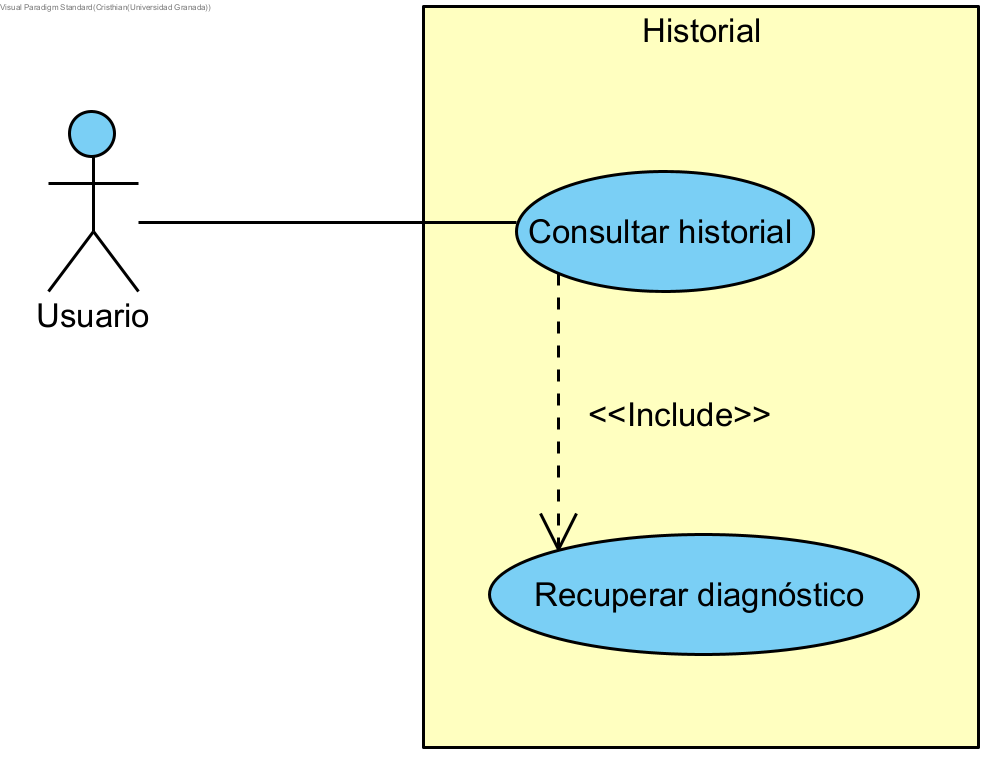
\includegraphics[scale = 1]{imagenes/Historial.png}
 	\caption{Caso de uso: Consulta de historial}
 	\label{fig:histcu}
 \end{figure}

Si agrupamos las funcionalidades en paquetes, podemos obtener un modelo visual que organiza los contenidos de los casos de uso en lo que  será la estructura del proyecto. El resultado es el diagrama de la figura \ref{fig:paquetes}.

\begin{figure}[H]
	\centering
	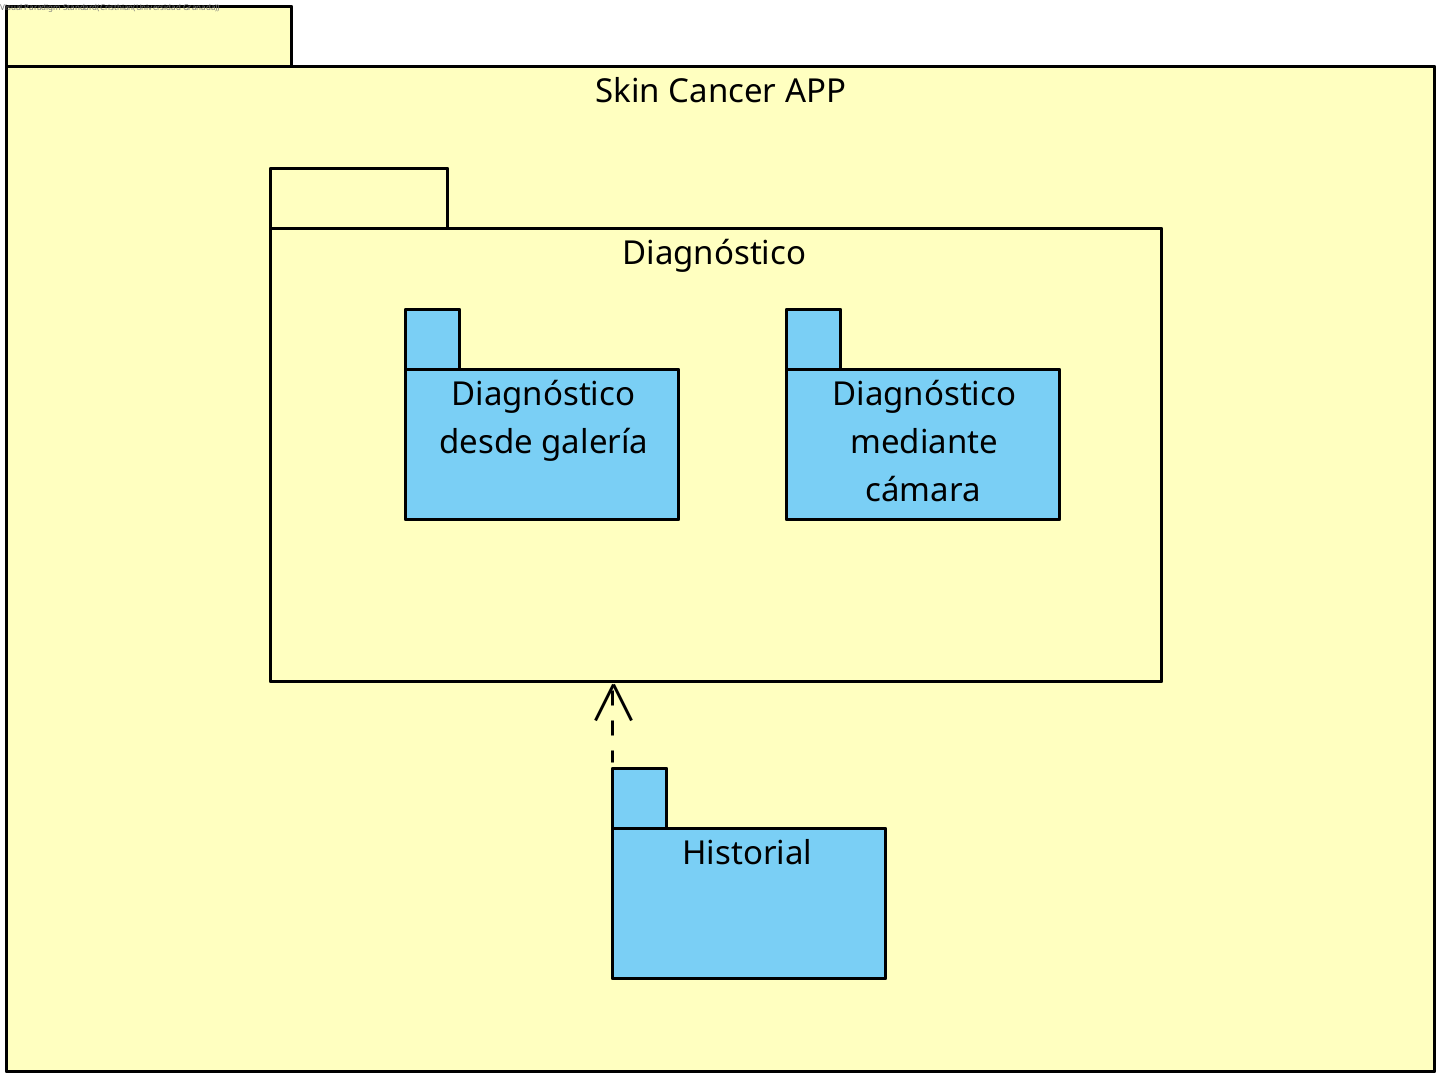
\includegraphics[scale = 0.7]{imagenes/DiagramaPaquetes.png}
	\caption{Diagrama de paquetes}
	\label{fig:paquetes}
\end{figure}

\subsection{Actores}

En el sistema que estamos diseñando, únicamente disponemos de un actor presente: el usuario, paciente de una enfermedad cutánea, que desea emplear el sistema para conocer qué enfermedad sufre en su piel. Se trata de una interacción directa con la aplicación, donde no intervienen otros actores humanos. En la tabla \ref{fig:actorusuario}, podemos apreciar una descripción detallada de sus características.

  \begin{table}[H]
	\centering
	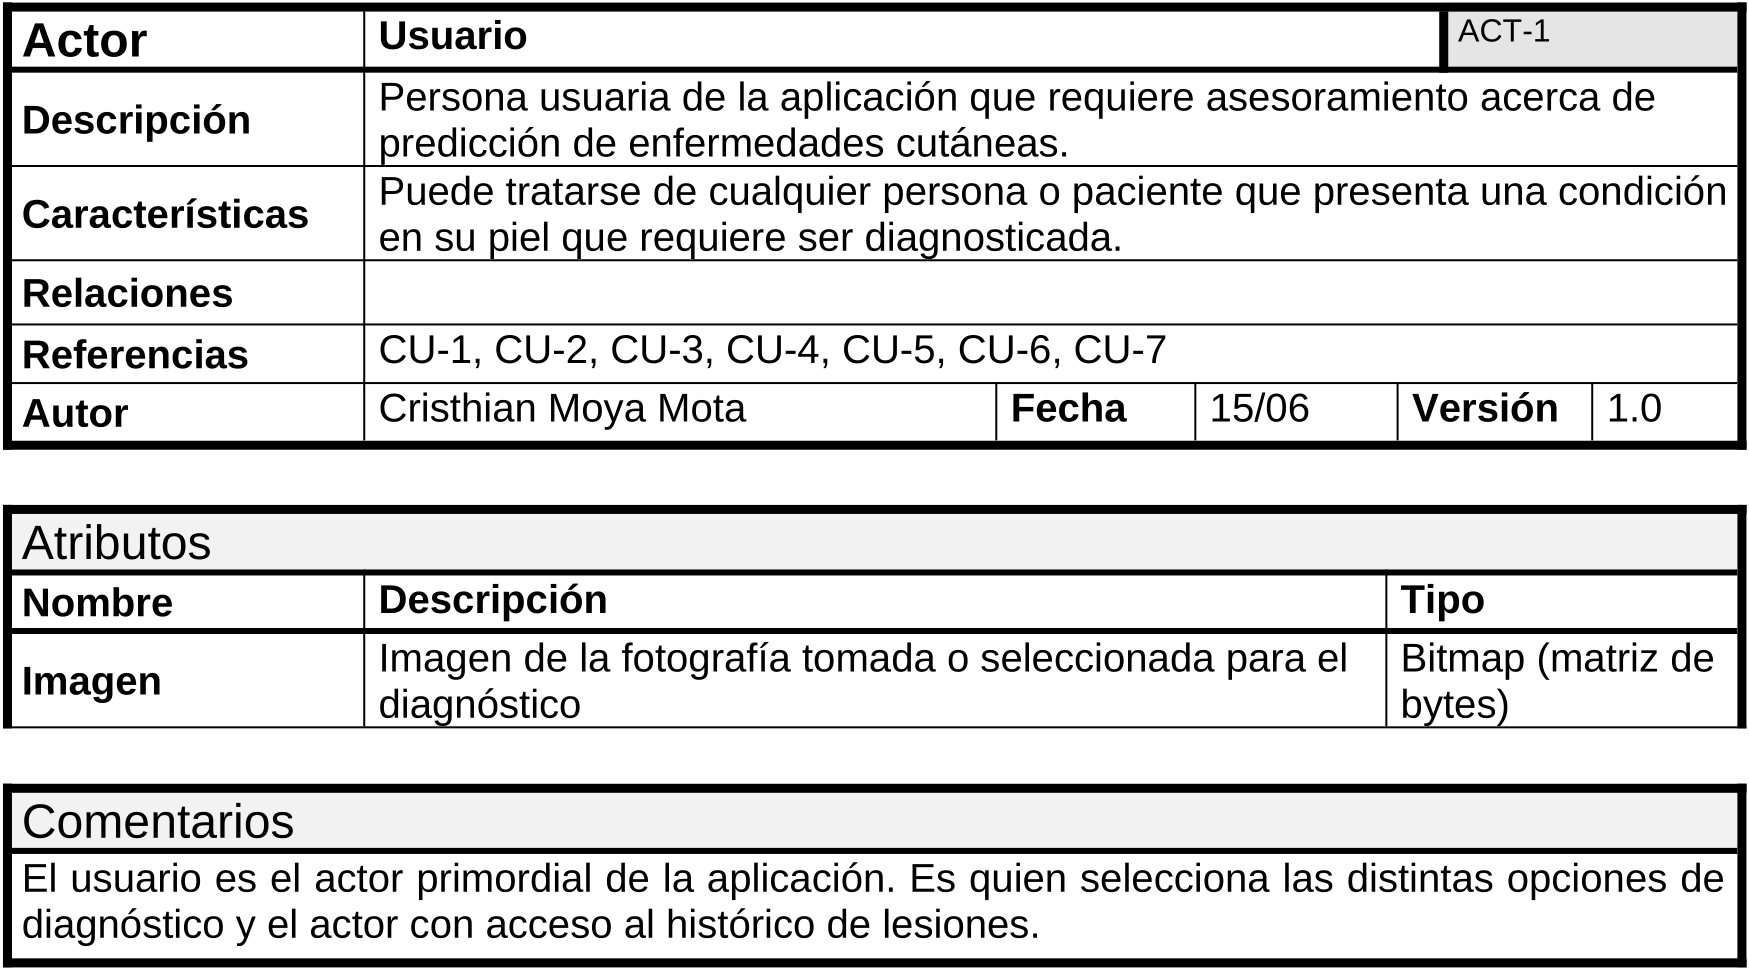
\includegraphics[scale = 0.225]{imagenes/tablausuario.png}
	\caption{Actor: usuario}
	\label{fig:actorusuario}
\end{table}

\subsection	{Descripción extendida de los casos de uso}

Para comprender adecuadamente las implicaciones de cada caso de uso, debemos de realizar un análisis en detalle del mismo. En las tablas mostradas a continuación, podemos observar numerados los 7 casos identificables: \textit{CU-1} (tabla \ref{fig:cu1}), \textit{CU-2} (tabla \ref{fig:cu2}), \textit{CU-3} (tabla \ref{fig:cu3}), \textit{CU-4} (tabla \ref{fig:cu4}), \textit{CU-5} (tabla \ref{fig:cu5}), \textit{CU-6} (tabla \ref{fig:cu6}) y \textit{CU-7} (tabla \ref{fig:cu7}).

  \begin{table}[H]
	\centering
	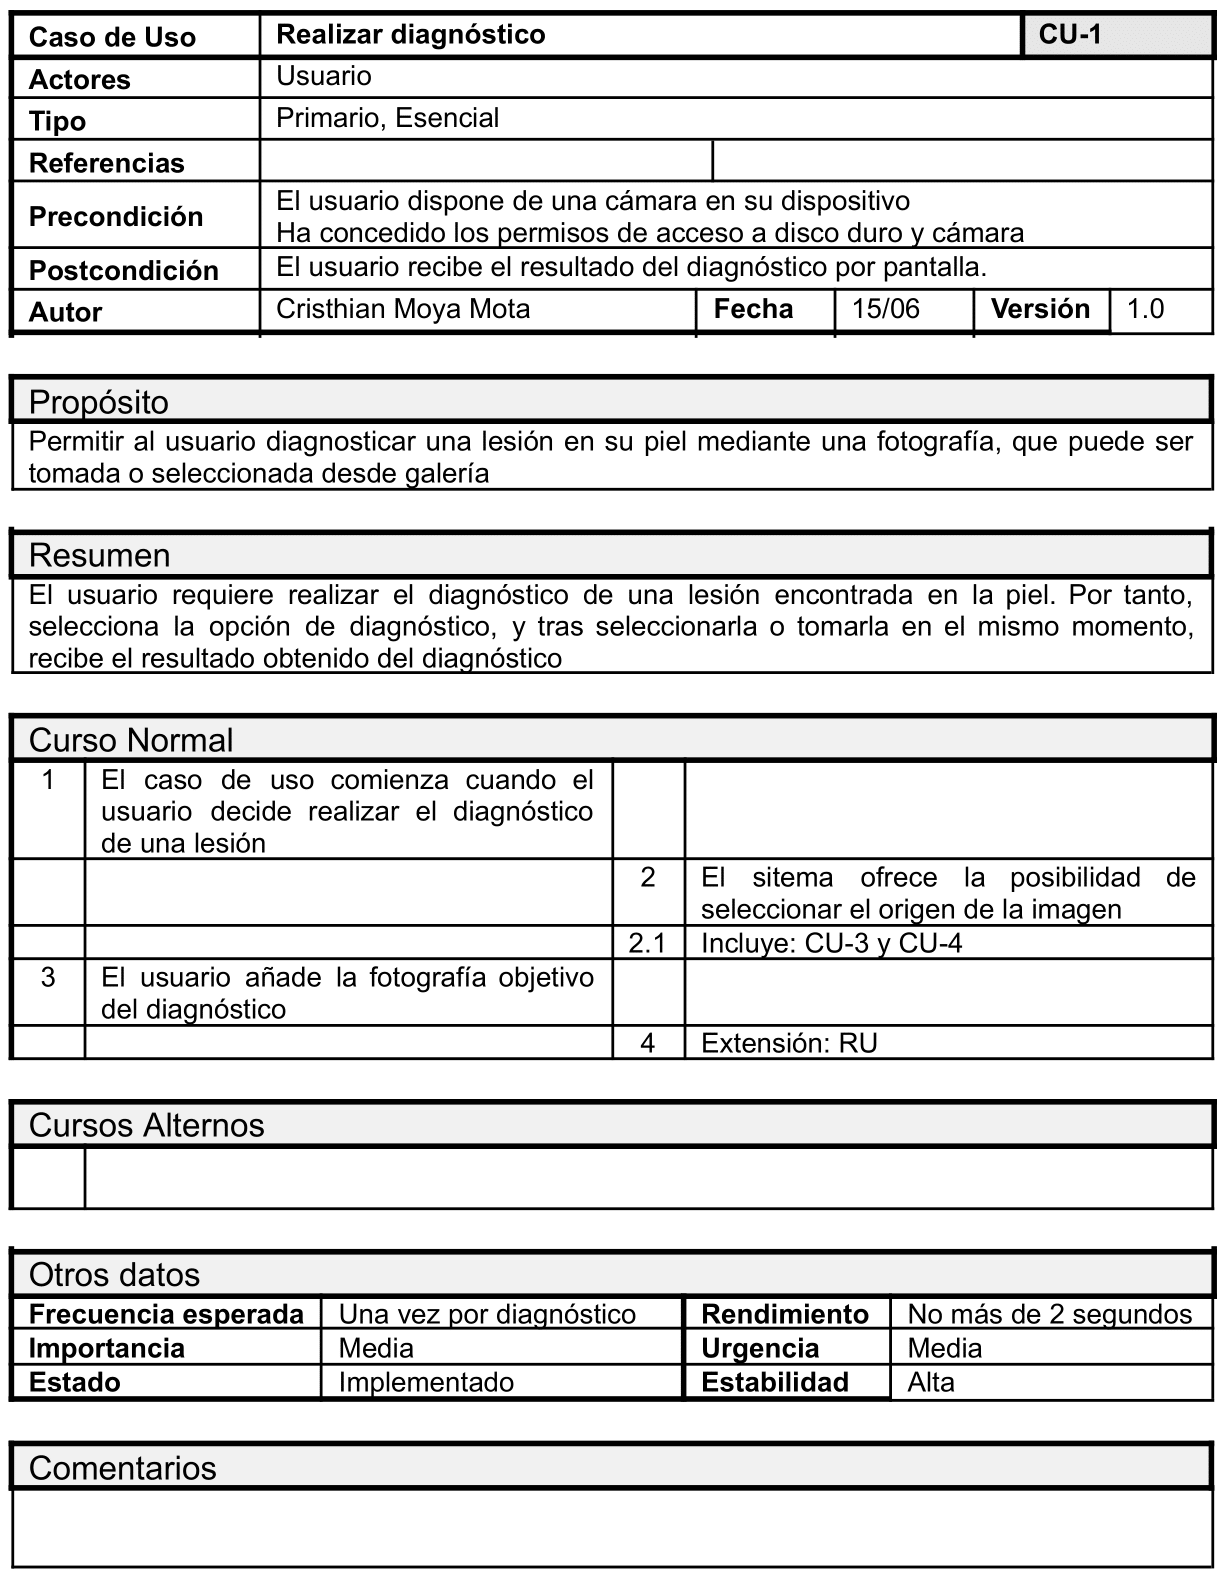
\includegraphics[scale=0.33]{imagenes/cu-1.png}
	\caption{Caso de uso CU-1: realizar diagnóstico}
	\label{fig:cu1}
\end{table}


  \begin{table}[H]
	\centering
	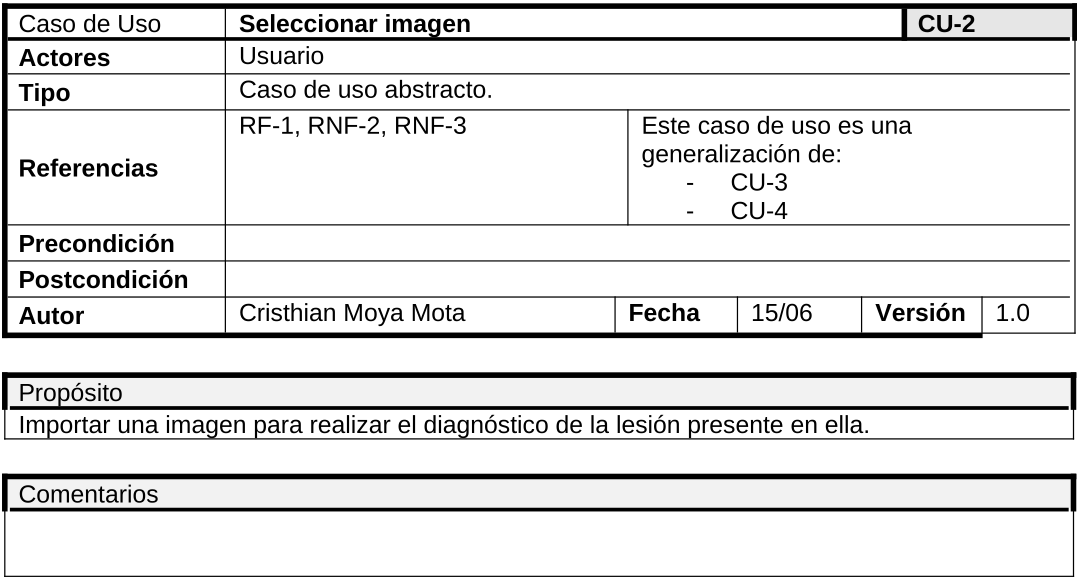
\includegraphics[scale=0.4]{imagenes/cu-2.png}
	\caption{Caso de uso CU-2: seleccionar imagen}
	\label{fig:cu2}
\end{table}

  \begin{table}[H]
	\centering
	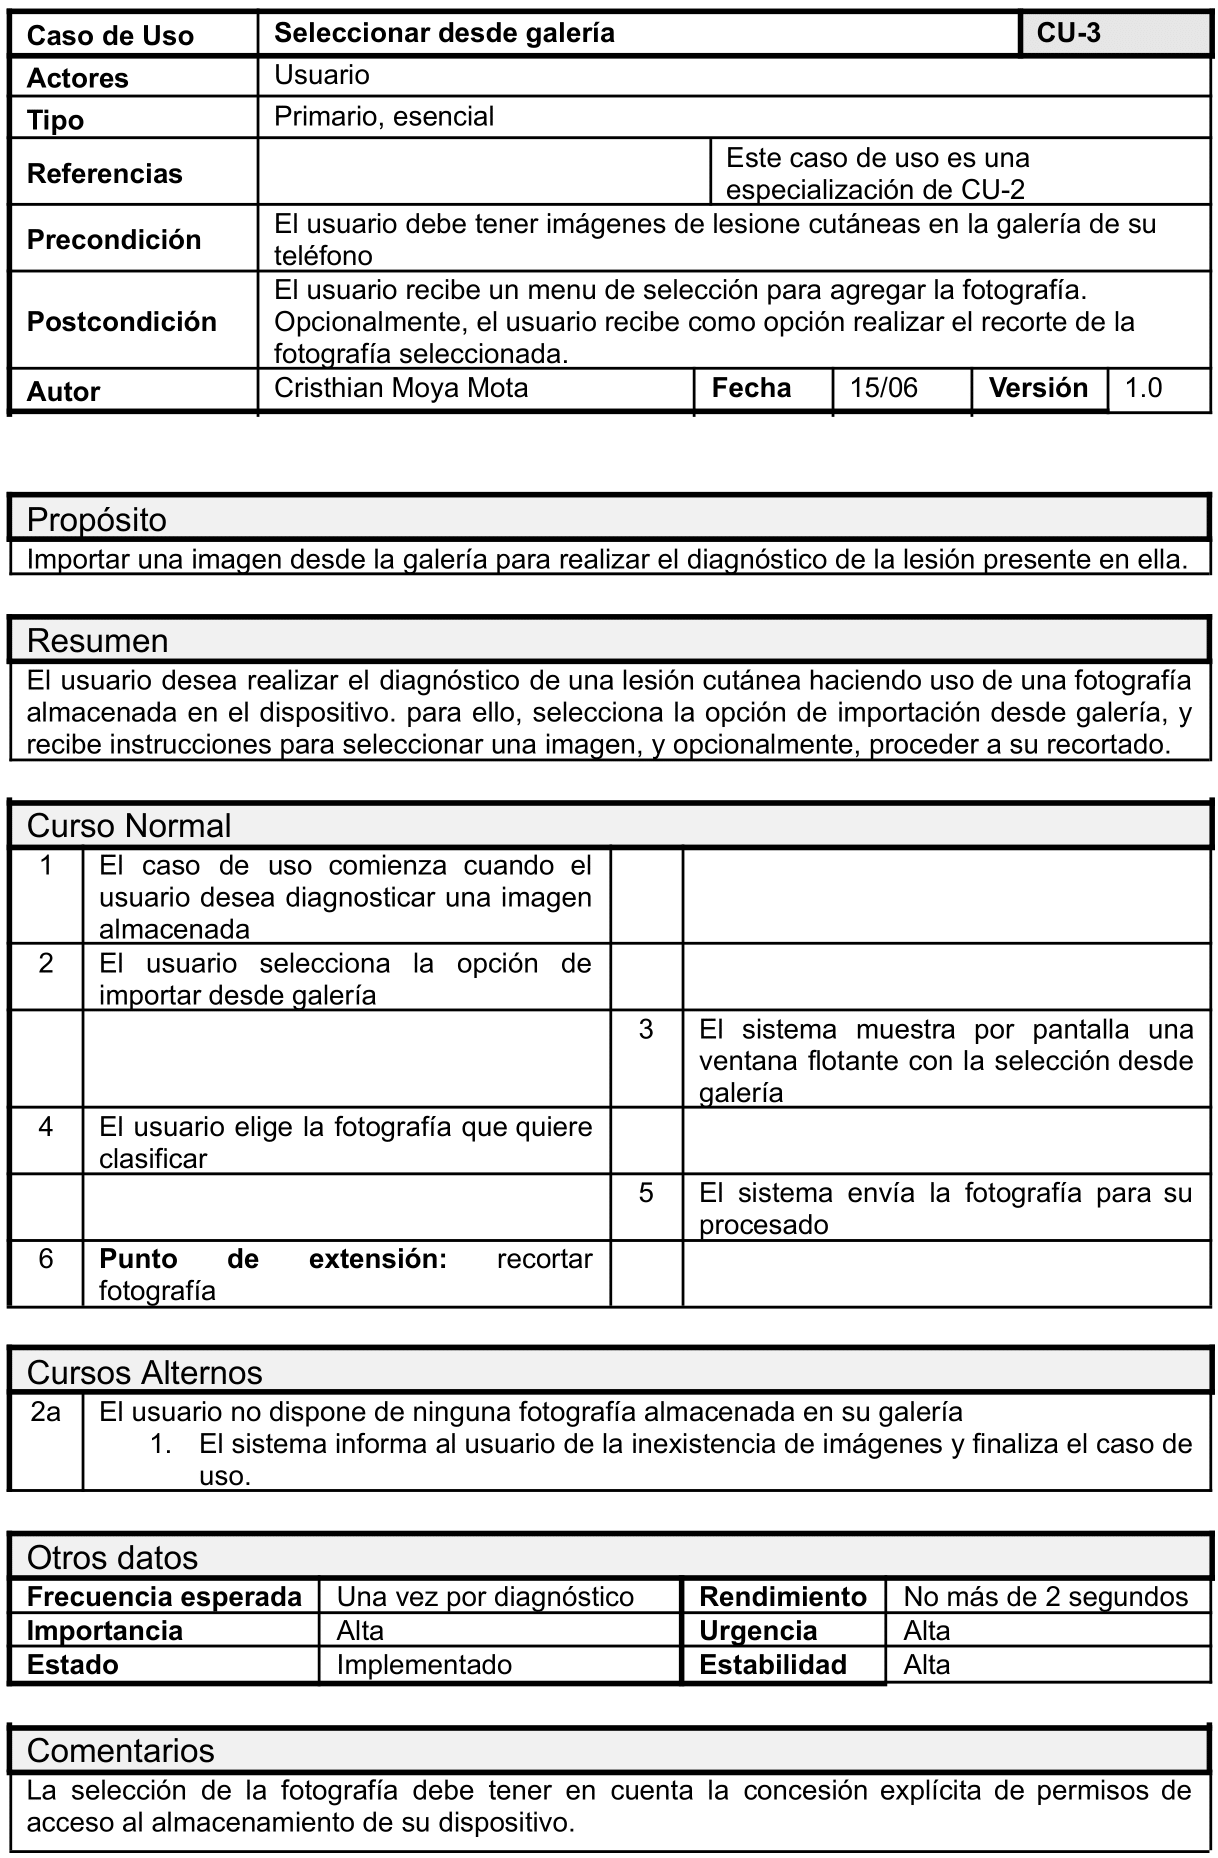
\includegraphics[scale=0.45]{imagenes/cu-3.png}
	\caption{Caso de uso CU-3: seleccionar desde galería}
	\label{fig:cu3}
\end{table}

  \begin{table}[H]
	\centering
	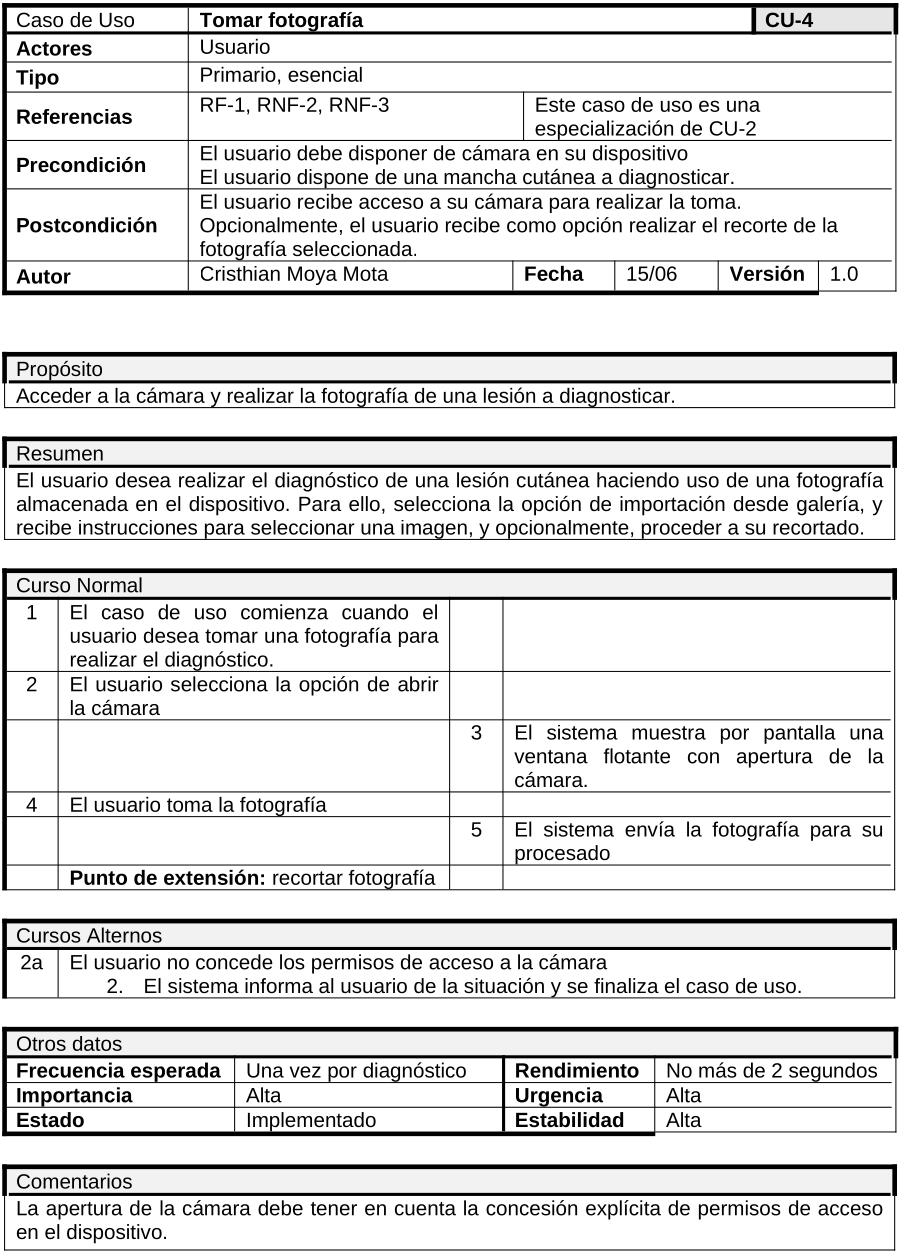
\includegraphics[scale=0.45]{imagenes/cu-4.png}
	\caption{Caso de uso CU-4: tomar fotografía}
	\label{fig:cu4}
\end{table}

  \begin{table}[H]
	\centering
	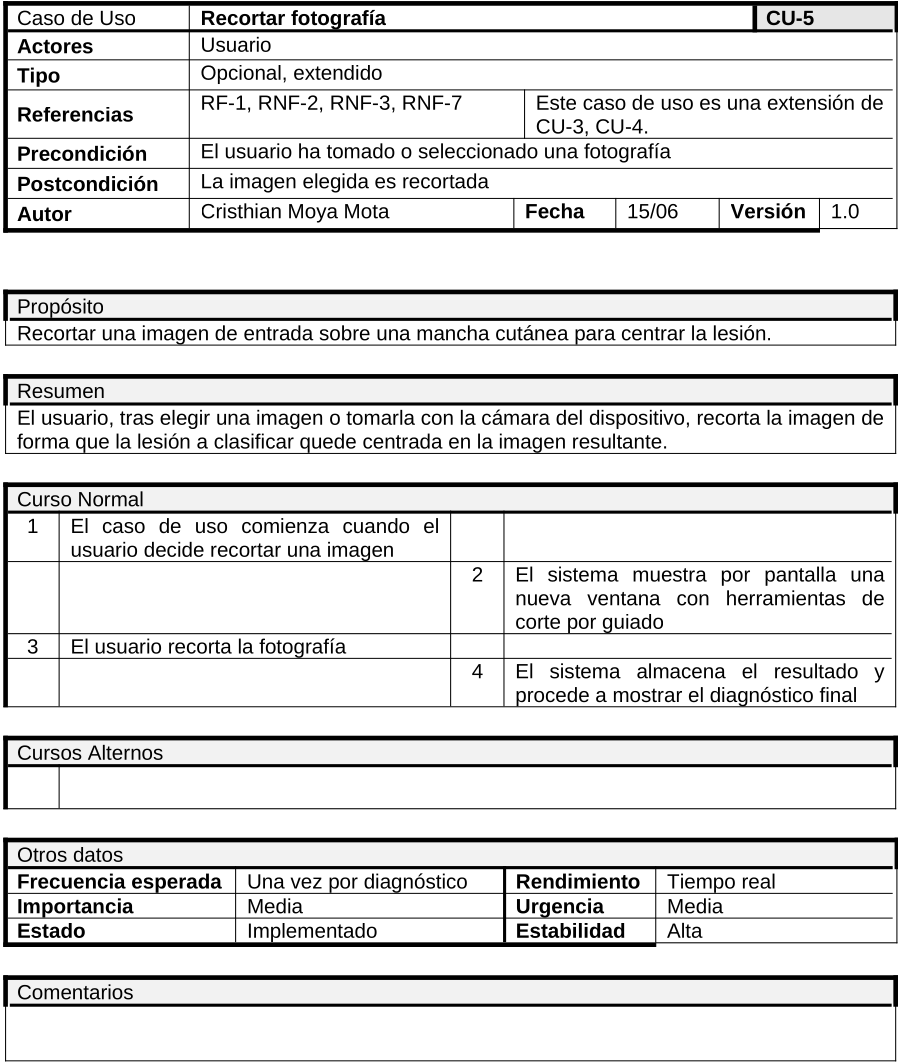
\includegraphics[scale=0.45]{imagenes/cu-5.png}
	\caption{Caso de uso CU-5: recortar región}
	\label{fig:cu5}
\end{table}

\begin{table}[H]
	\centering
	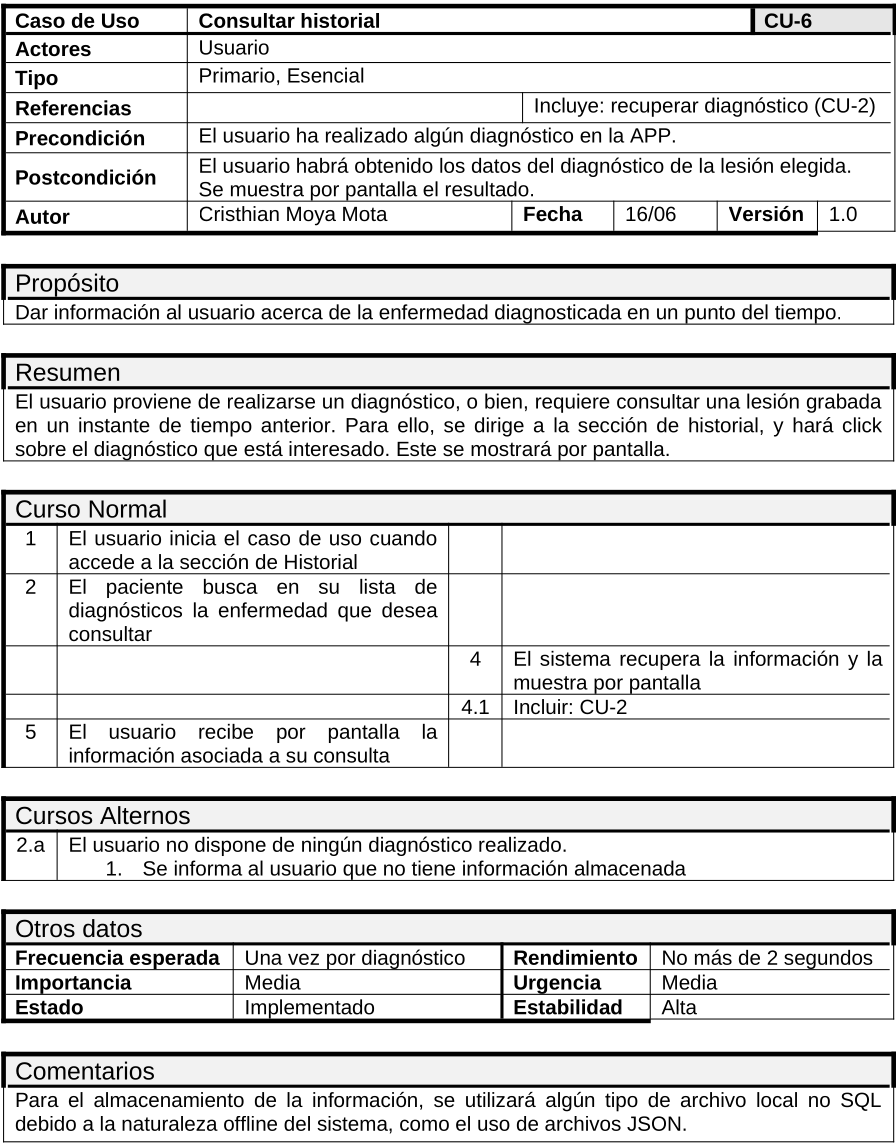
\includegraphics[scale=0.45]{imagenes/cu-6.png}
	\caption{Caso de uso CU-6: consultar historial}
	\label{fig:cu6}
\end{table}

\begin{table}[H]
	\centering
	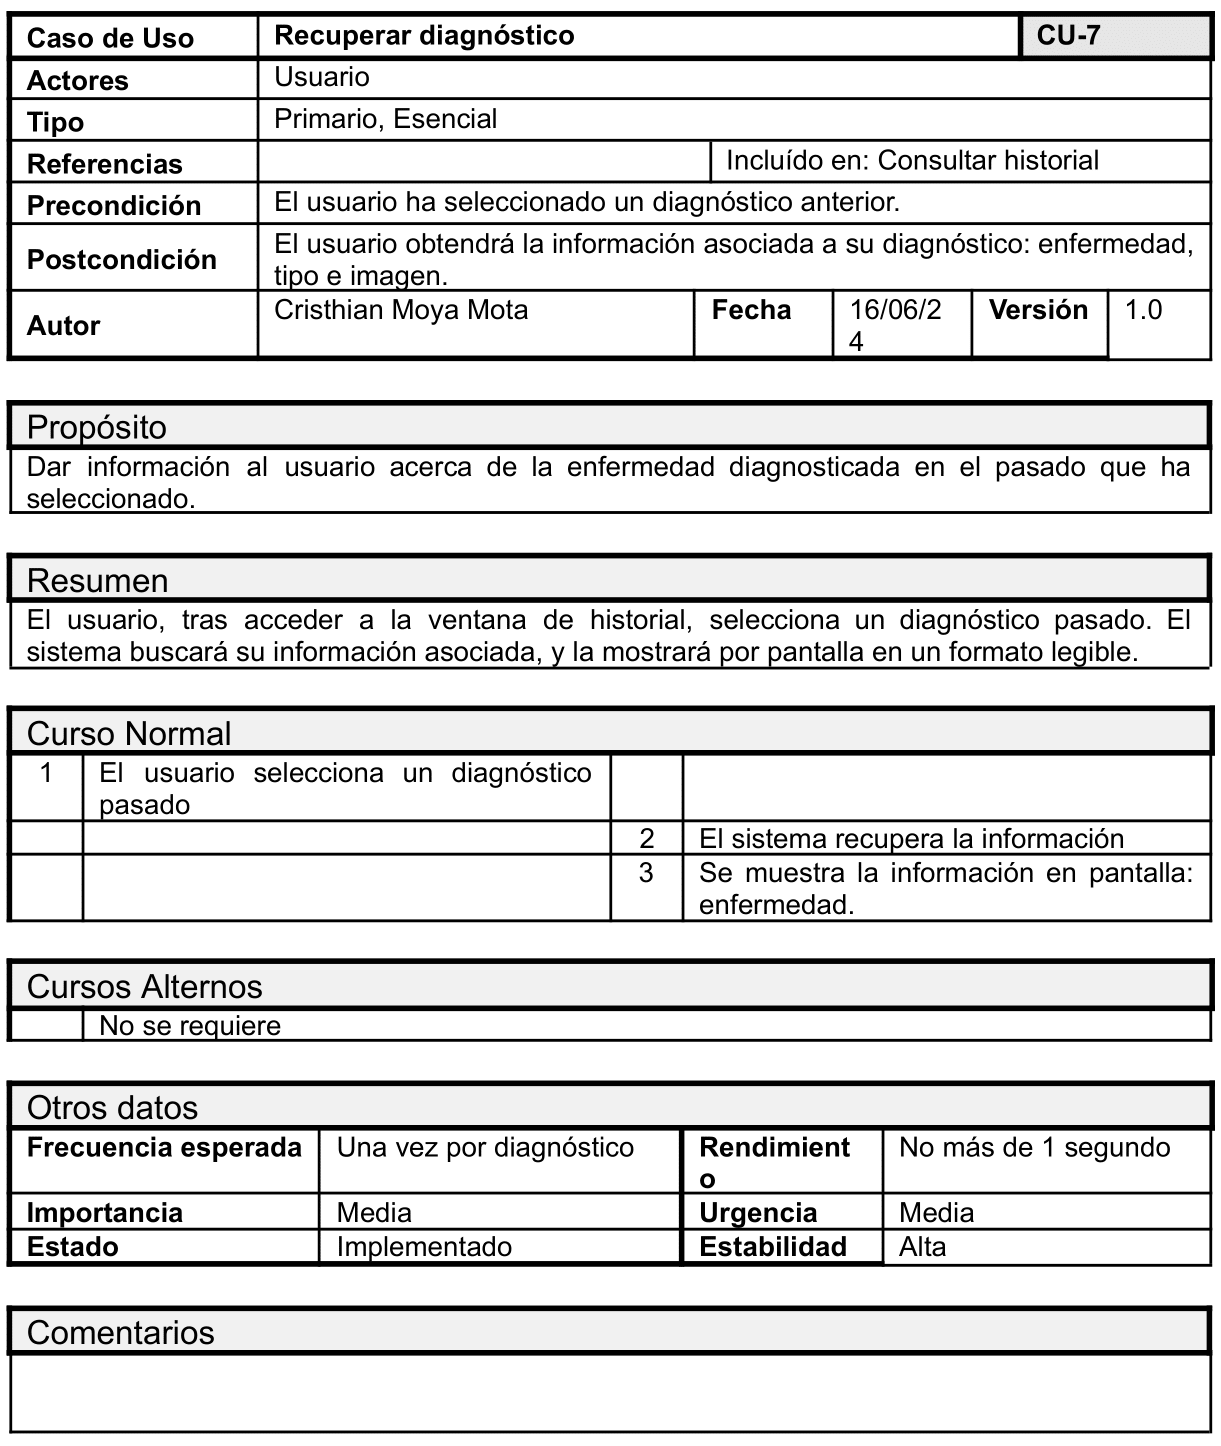
\includegraphics[scale=0.375]{imagenes/cu-7.png}
	\caption{Caso de uso CU-7: recuperar diagnóstico}
	\label{fig:cu7}
\end{table}

De esta forma, ya disponemos de las interacciones detalladas que existen entre cada uno de los casos de uso, y podemos elaborar el diagrama de concepto asociado que nos describe la cardinalidad de las mismas. Dicho diagrama, se convertirá posteriormente en la base para la creación del diagrama de clases de diseño.

\section{Modelo de análisis}
Una vez hemos descrito adecuadamente los casos de uso obtenidos, podemos pasar a la fase de análisis del problema. En esta fase, una vez se han detectado todos los requisitos, procedemos a representarlos formalmente mediante modelos. Concretamente, tenemos dos tipos de modelos: estático y dinámico.

\begin{enumerate}
	\item \textbf{Modelo estático}.  Muestra la estructura que sigue el proyecto, a través de un modelo conceptual, donde se relacionan las distintas entidades detectadas en el problema. Se representa a través de un diagrama conceptual.
	\item \textbf{Modelo dinámico}. Representa las relaciones que se producen durante el uso del proyecto, es decir, representan el comportamiento del mismo. Se hace uso de los diagramas de secuencia y los contratos de diseño.
\end{enumerate} 

Comenzaremos por la especificación del diagrama conceptual, y posteriormente el comportamiento dinámico del sistema.

\subsection{Modelo estático: diagrama conceptual}

Para la especificación del modelo estático, debemos realizar una análisis de los conceptos que componen el sistema, e identificar aquellos que verdaderamente participan en él. De esta forma, podemos construir el diagrama de conceptual, y representar de manera estática la estructura del proyecto.

Atendiendo a los objetivos especificados en el capítulo \ref{cap:objetivos} y la descripción del problema que extendimos en el apartado \ref{sec:descripcion}, podemos identificar los siguientes conceptos clave:

\begin{itemize}
	\item \textbf{Imagen}. Elemento clave del sistema, sobre el cual se realiza la clasificación de la enfermedad.  A su vez, podemos encontrar dos tipos muy similares, pero con distintos tipos de almacenaje: \textbf{ImagenDisco} e \textbf{ImagenCámara}, siendo la primera obtenida a partir de su dirección URI (identificador de recursos uniforme, i.e, una dirección única), y la segunda, directamente como mapa de bits procedente de la cámara.
	\item  \textbf{Patología} (llamada como \textbf{InfoPatología}). Información asociada a la enfermedad que el usuario recibe como descripción.
	\item \textbf{Diagnóstico} (llamado como \textbf{DiagnósticoData}). Información completa, que incluye la descripción de la patología, y la imagen asociada, cuyo objetivo es ser almacenado en el historial para ser recuperado cuando se desee.
	\item \textbf{Historial}. Estructura de información que puede contener ninguno o varios diagnósticos previamente realizados de forma que el usuario pueda consultar la evolución de su enfermedad, o buscar antiguas prognosis.
\end{itemize}

De esta forma, nos queda el diagrama conceptual apreciable en la figura \ref{fig:conceptual}.

\begin{figure}[H]
	\centering
	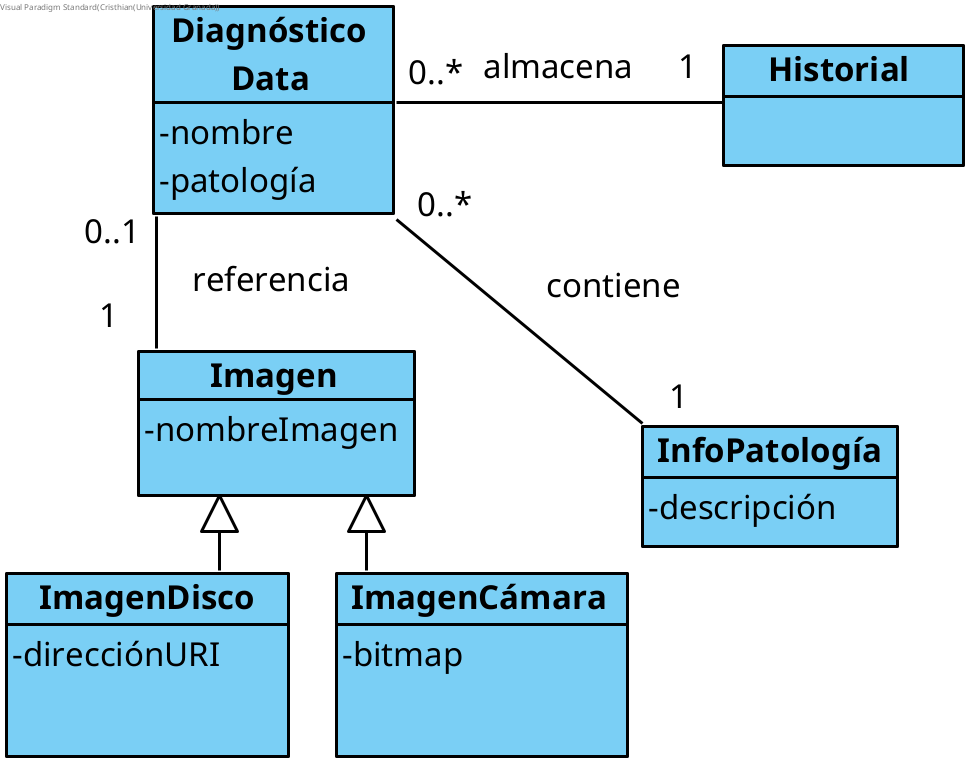
\includegraphics[scale = 1.2]{imagenes/MapaConceptual.png}
	\caption{Diagrama conceptual}
	\label{fig:conceptual}
\end{figure}

\subsection{Modelo dinámico: diagramas de secuencia y contratos}

En esta sección, estudiaremos las interacciones entre las diferentes partes del sistema. Para ello, emplearemos los diagramas de secuencia y los contratos de C. Larman \cite{larman2003uml}.

\subsubsection{Diagrama de secuencia}
En un diagrama de secuencia, se muestran como los eventos que generan los actores del sistema provocan la ejecución de una operación por el sistema, siendo visto este como una caja negra. En nuestro caso, las acciones son bastante limitadas, ya que únicamente disponemos de un actor: el usuario de la aplicación. 

Partiendo de las acciones definidas en los casos de uso, junto con los posibles parámetros de entrada que puede requerir cada evento producido. En este caso, además, se ha empleado el uso de un diagrama de secuencia por cada diagrama de casos de uso, de forma que ya quede establecida la separación de funcionalidades.

En la figura \ref{fig:secdiag} podemos apreciar el diagrama de secuencia asociado al diagnóstico, mientras que en la figura \ref{fig:sechistorial}, se represente el diagrama para el subsistema del historial.

\begin{figure}[H]
	\centering
	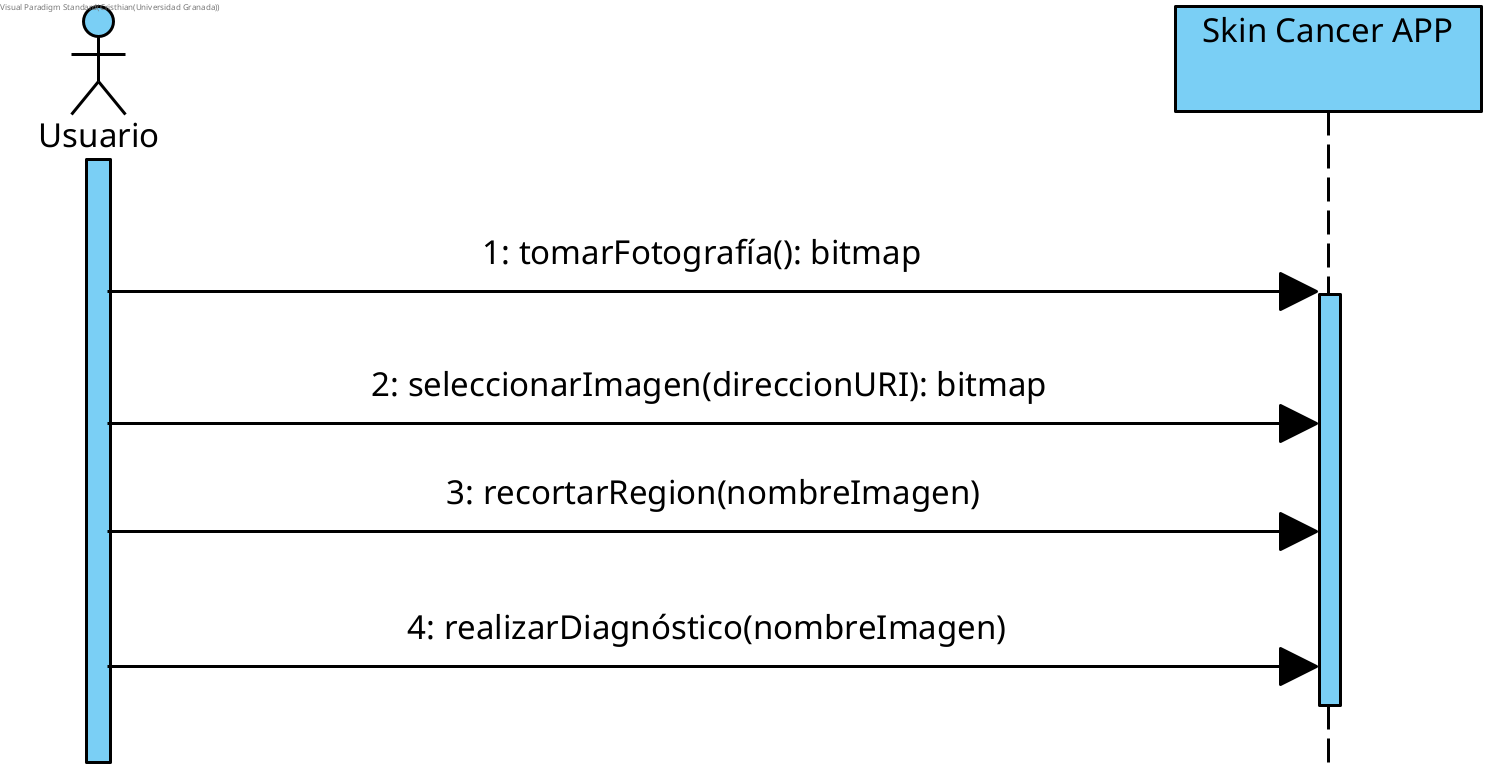
\includegraphics[scale = 1]{imagenes/DiagramaSecuenciaFotografia.png}
	\caption{Diagrama de secuencia para el subsistema de fotografías y diagnóstico.}
	\label{fig:secdiag}
\end{figure}

\begin{figure}[H]
	\centering
	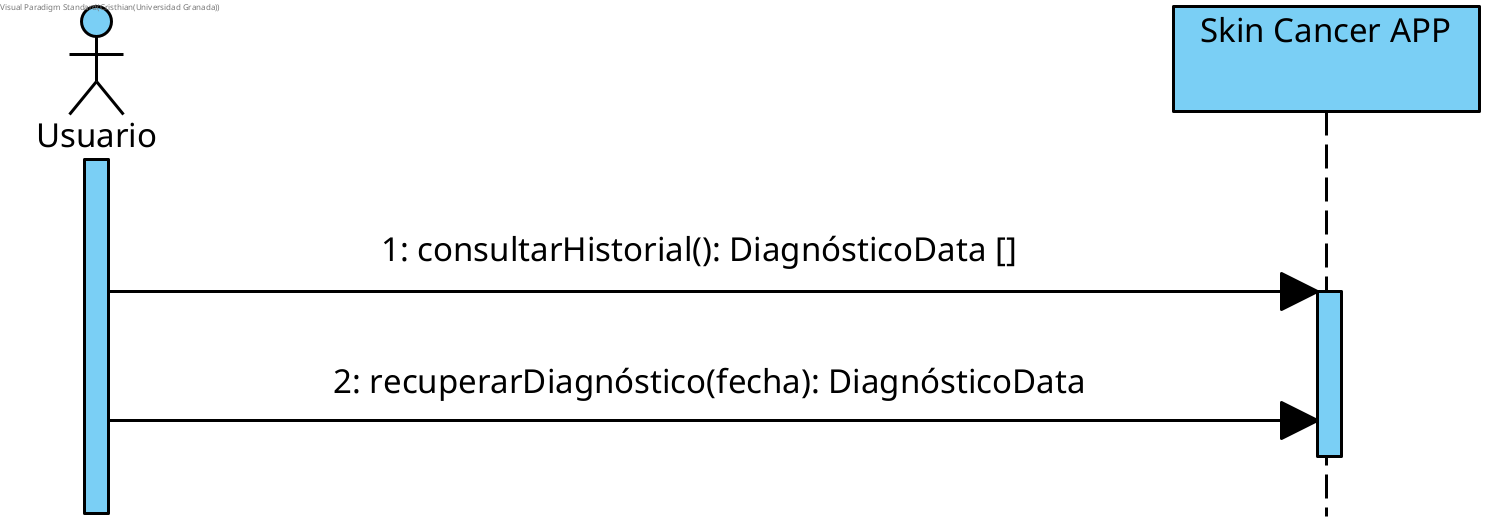
\includegraphics[scale = 1]{imagenes/DiagramaSecuenciaHistorial.png}
	\caption{Diagrama de secuencia para el subsistema de historial.}
	\label{fig:sechistorial}
\end{figure}

 \subsubsection{Contratos}
 
 Una vez queda representado visualmente los eventos que el usuario puede iniciar en el sistema mediante el diagrama de secuencia, debemos	de especificar lo que se desea lograr en cada operación realizada, pero aún sin entrar en detalles de su implementación. No existe un formato estandarizado único como sí lo ha sido hasta ahora el caso de los diagramas UML (Lenguaje unificado de modelado) con los diagramas de caso de uso y los de secuencia. Sin embargo, habitualmente se emplean los contratos de C. Larman \cite{larman2003uml}, donde se presentan las especificaciones de cada operación en un estilo declarativo, y comúnmente estructurado en formato de tabla.
 
 Para cada evento descrito en el modelo de secuencia, obtenemos su correspondiente contrato, que incluirá principalmente las precondiciones, excepciones, descripción de la operación, y postcondiciones que se producen en el sistema.
 
 En este proyecto, obtenemos 6 contratos, representados en las tablas \ref{fig:contrato1}, \ref{fig:contrato2}, \ref{fig:contrato3}, \ref{fig:contrato4}, \ref{fig:contrato5} y \ref{fig:contrato6}, siguiendo el orden de los eventos especificados en los diagramas de secuencia \ref{fig:secdiag} y \ref{fig:sechistorial}.
 
 \begin{table}[H]
 	\centering
 	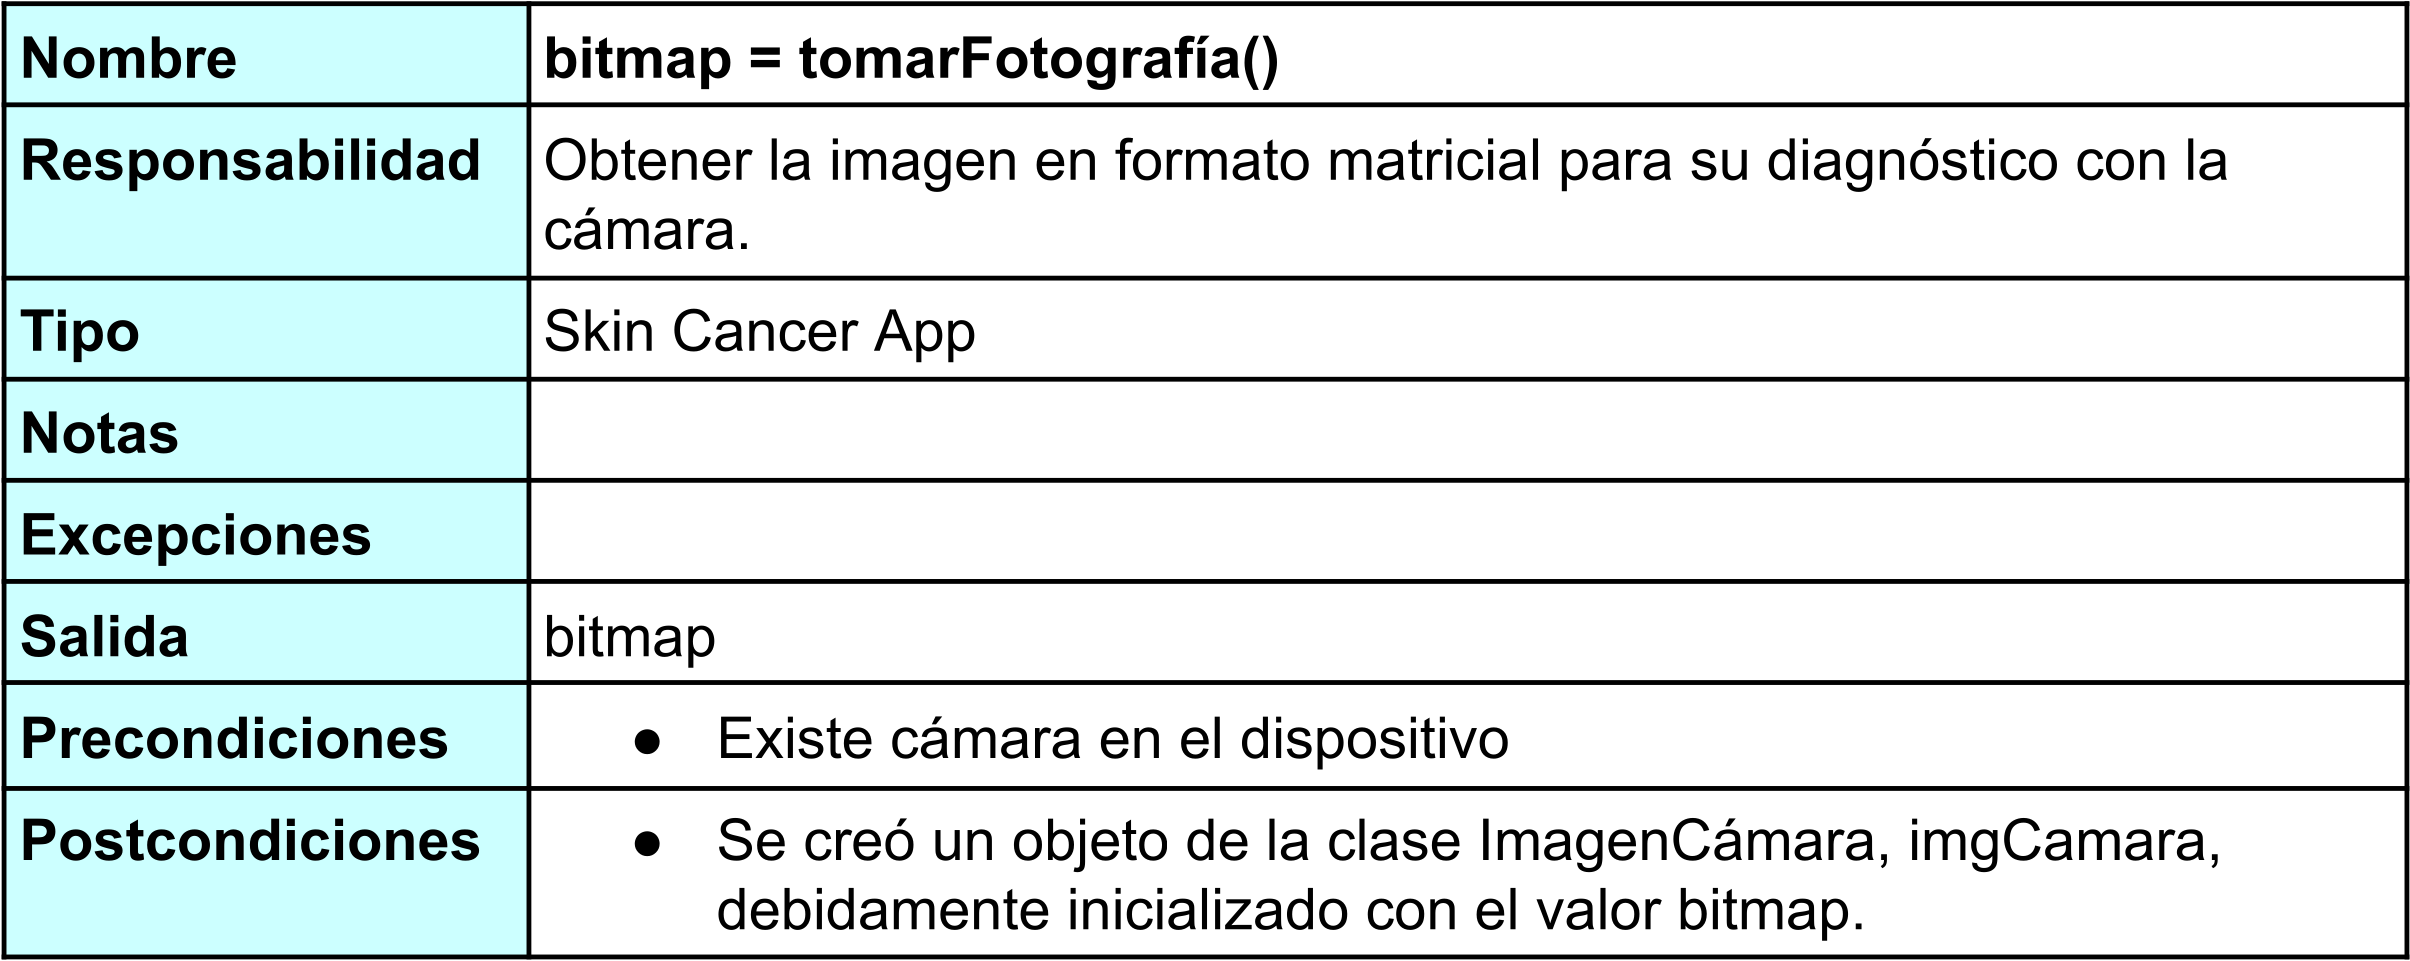
\includegraphics[scale = 0.16]{imagenes/contrato1.png}
 	\caption{Contrato: tomar fotografía.}
 	\label{fig:contrato1}
 \end{table}
 
  \begin{table}[H]
 	\centering
 	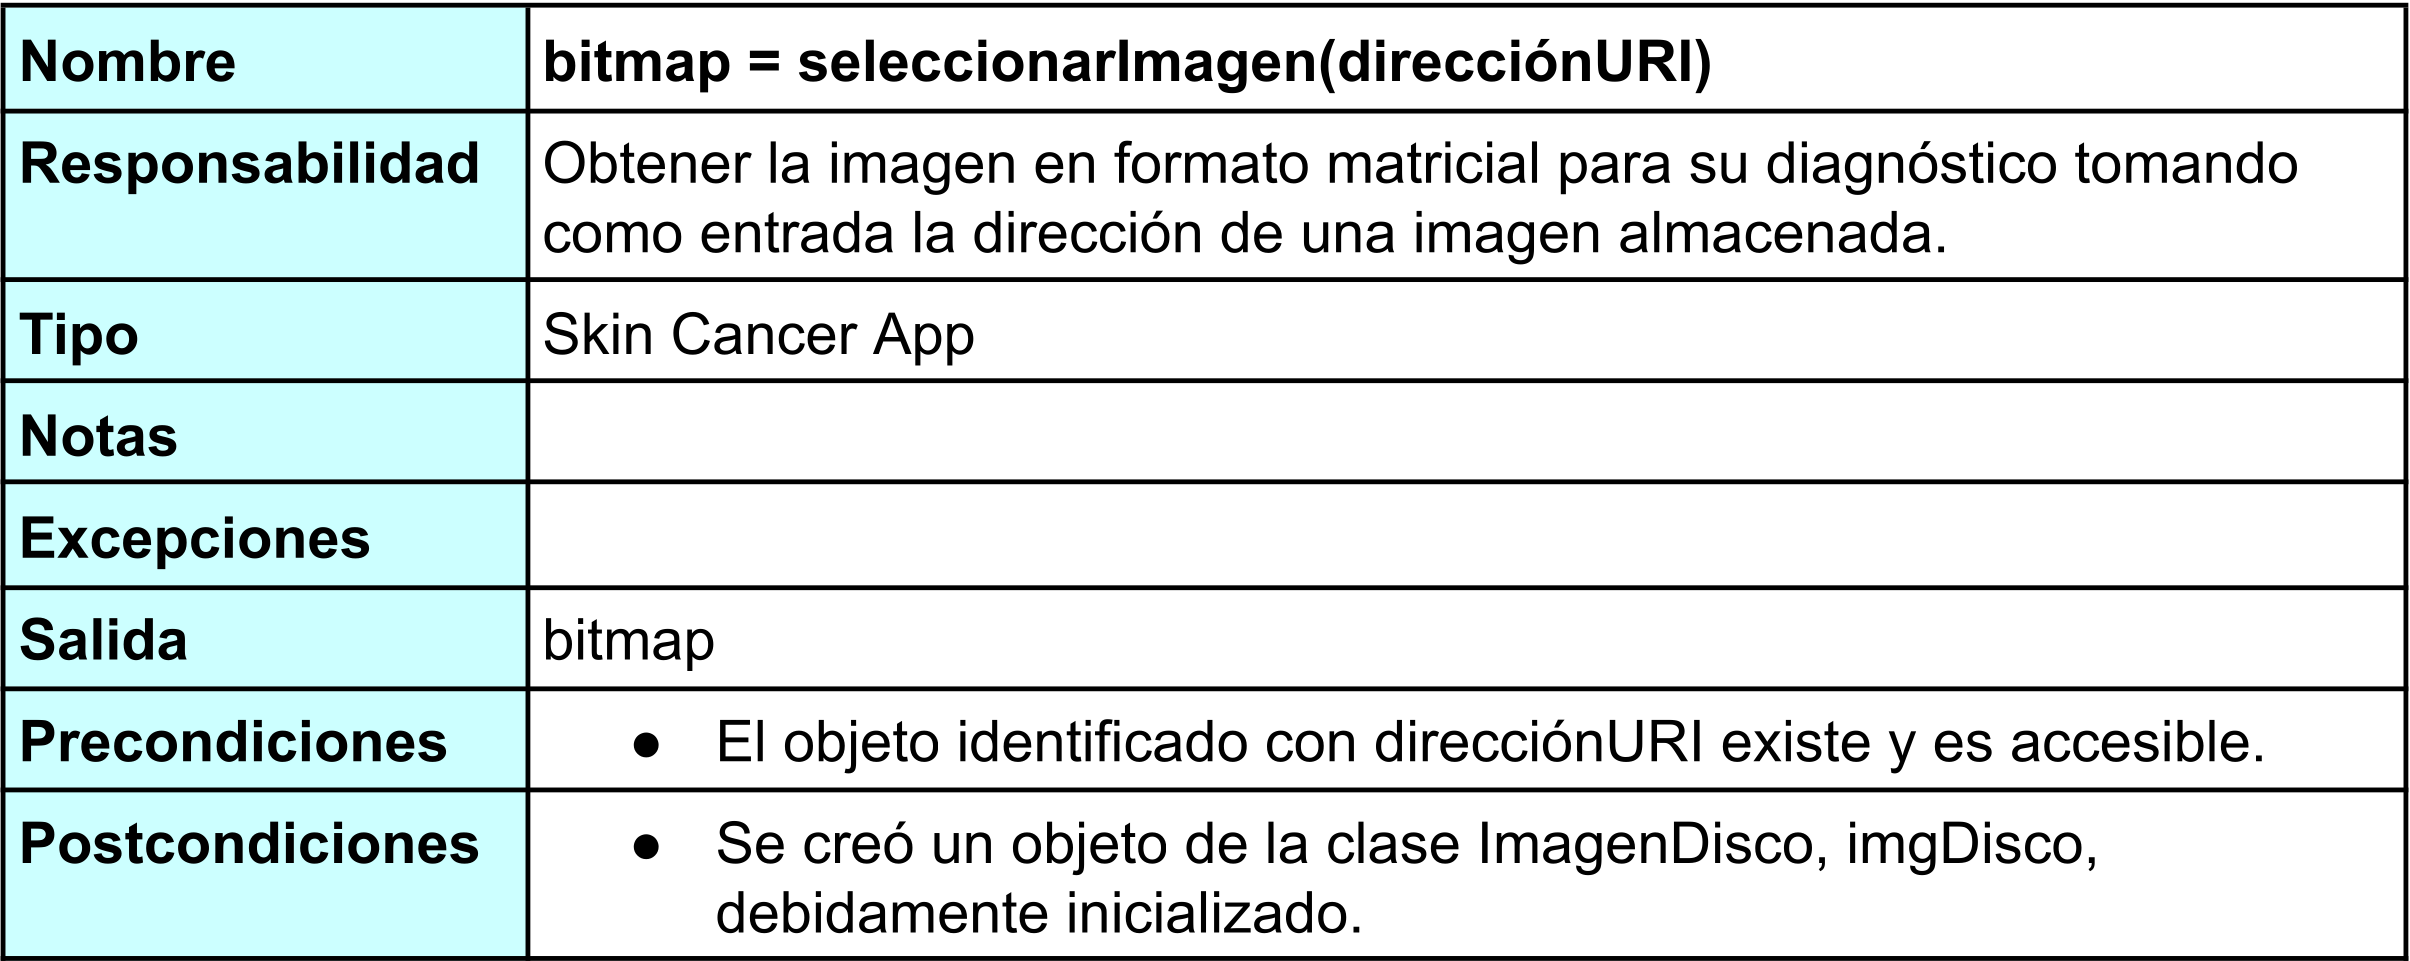
\includegraphics[scale = 0.16]{imagenes/contrato2.png}
 	\caption{Contrato: seleccionar imagen.}
 	\label{fig:contrato2}
 \end{table}
 
   \begin{table}[H]
 	\centering
 	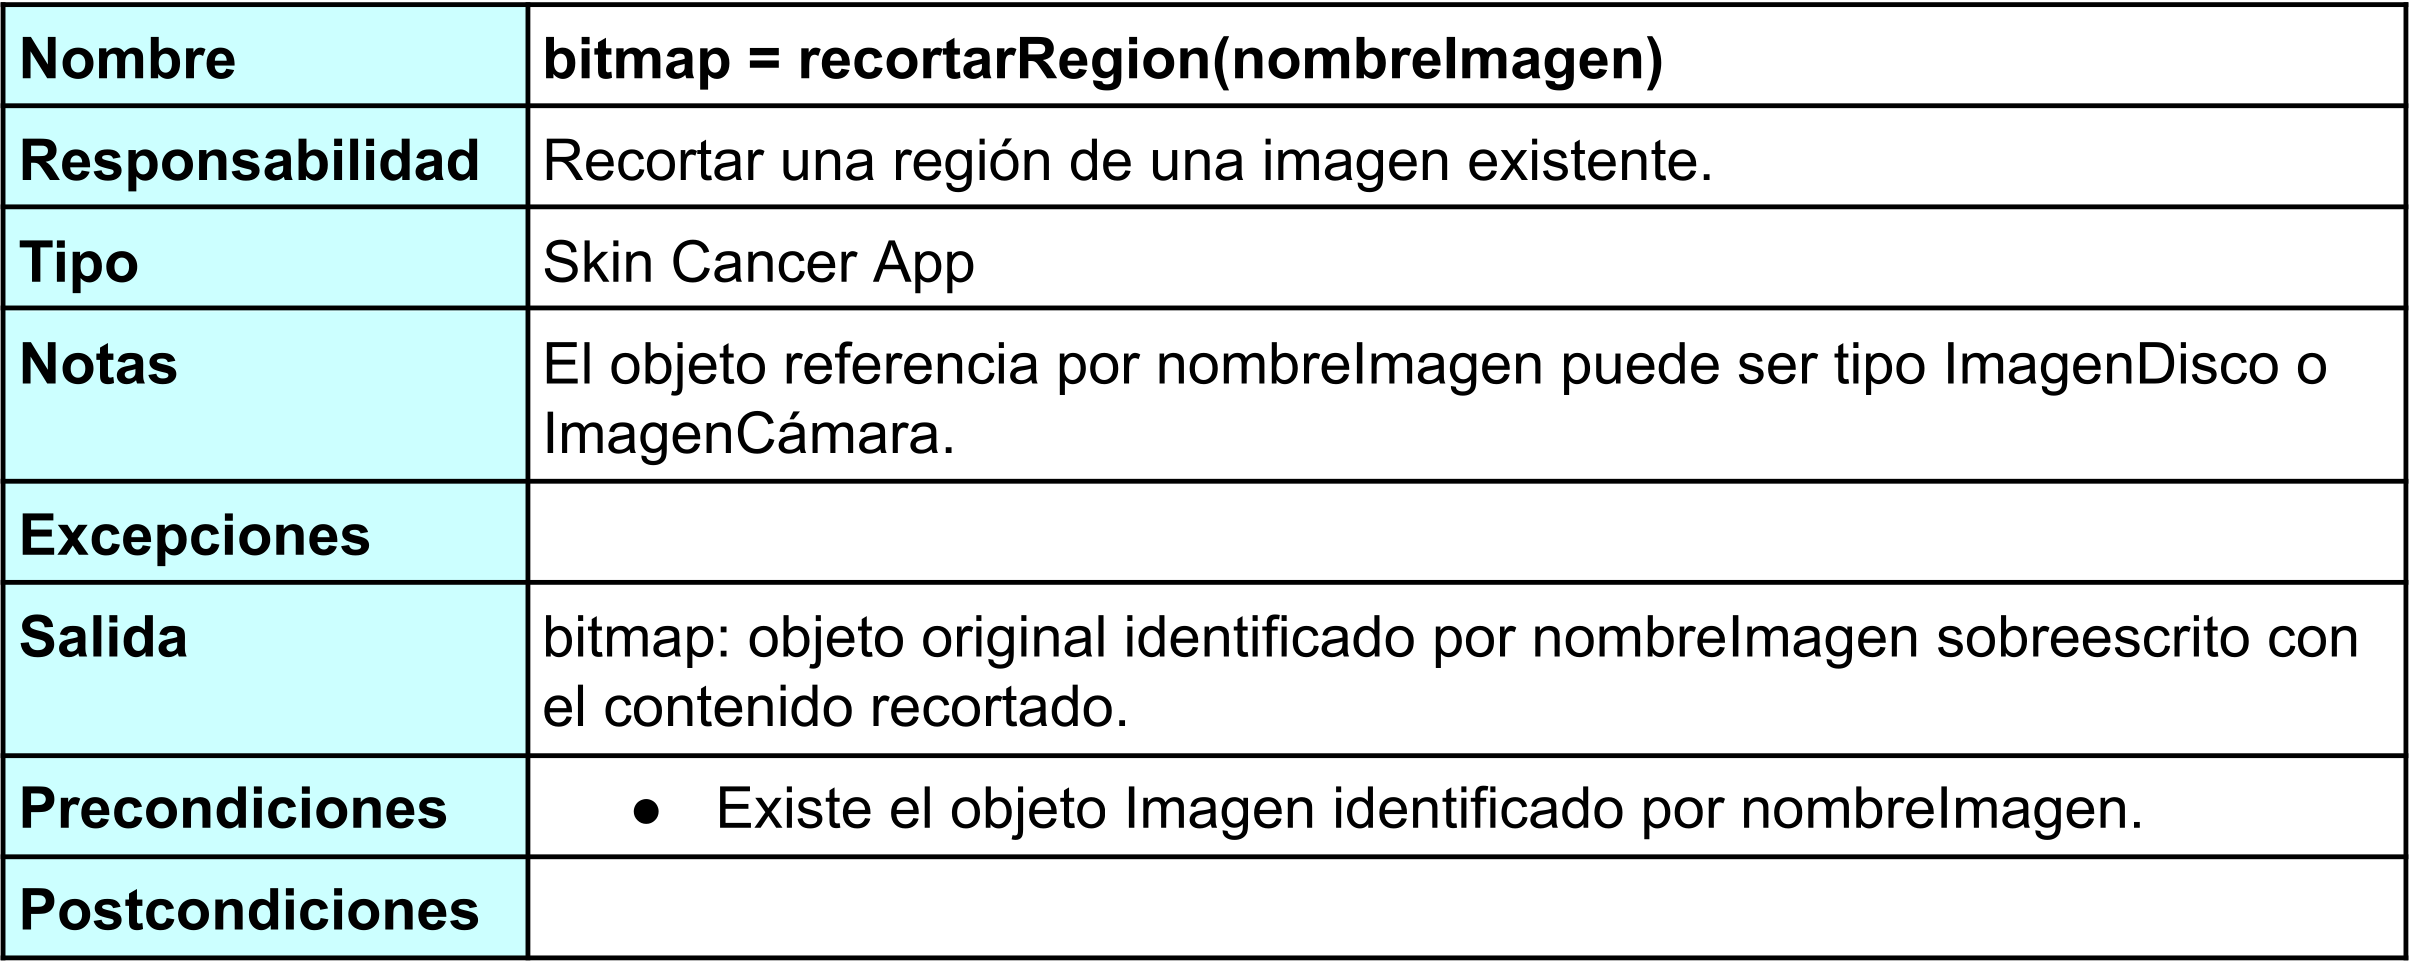
\includegraphics[scale = 0.16]{imagenes/contrato3.png}
 	\caption{Contrato: recortar región de una imagen.}
 	\label{fig:contrato3}
 \end{table}
 
   \begin{table}[H]
 	\centering
 	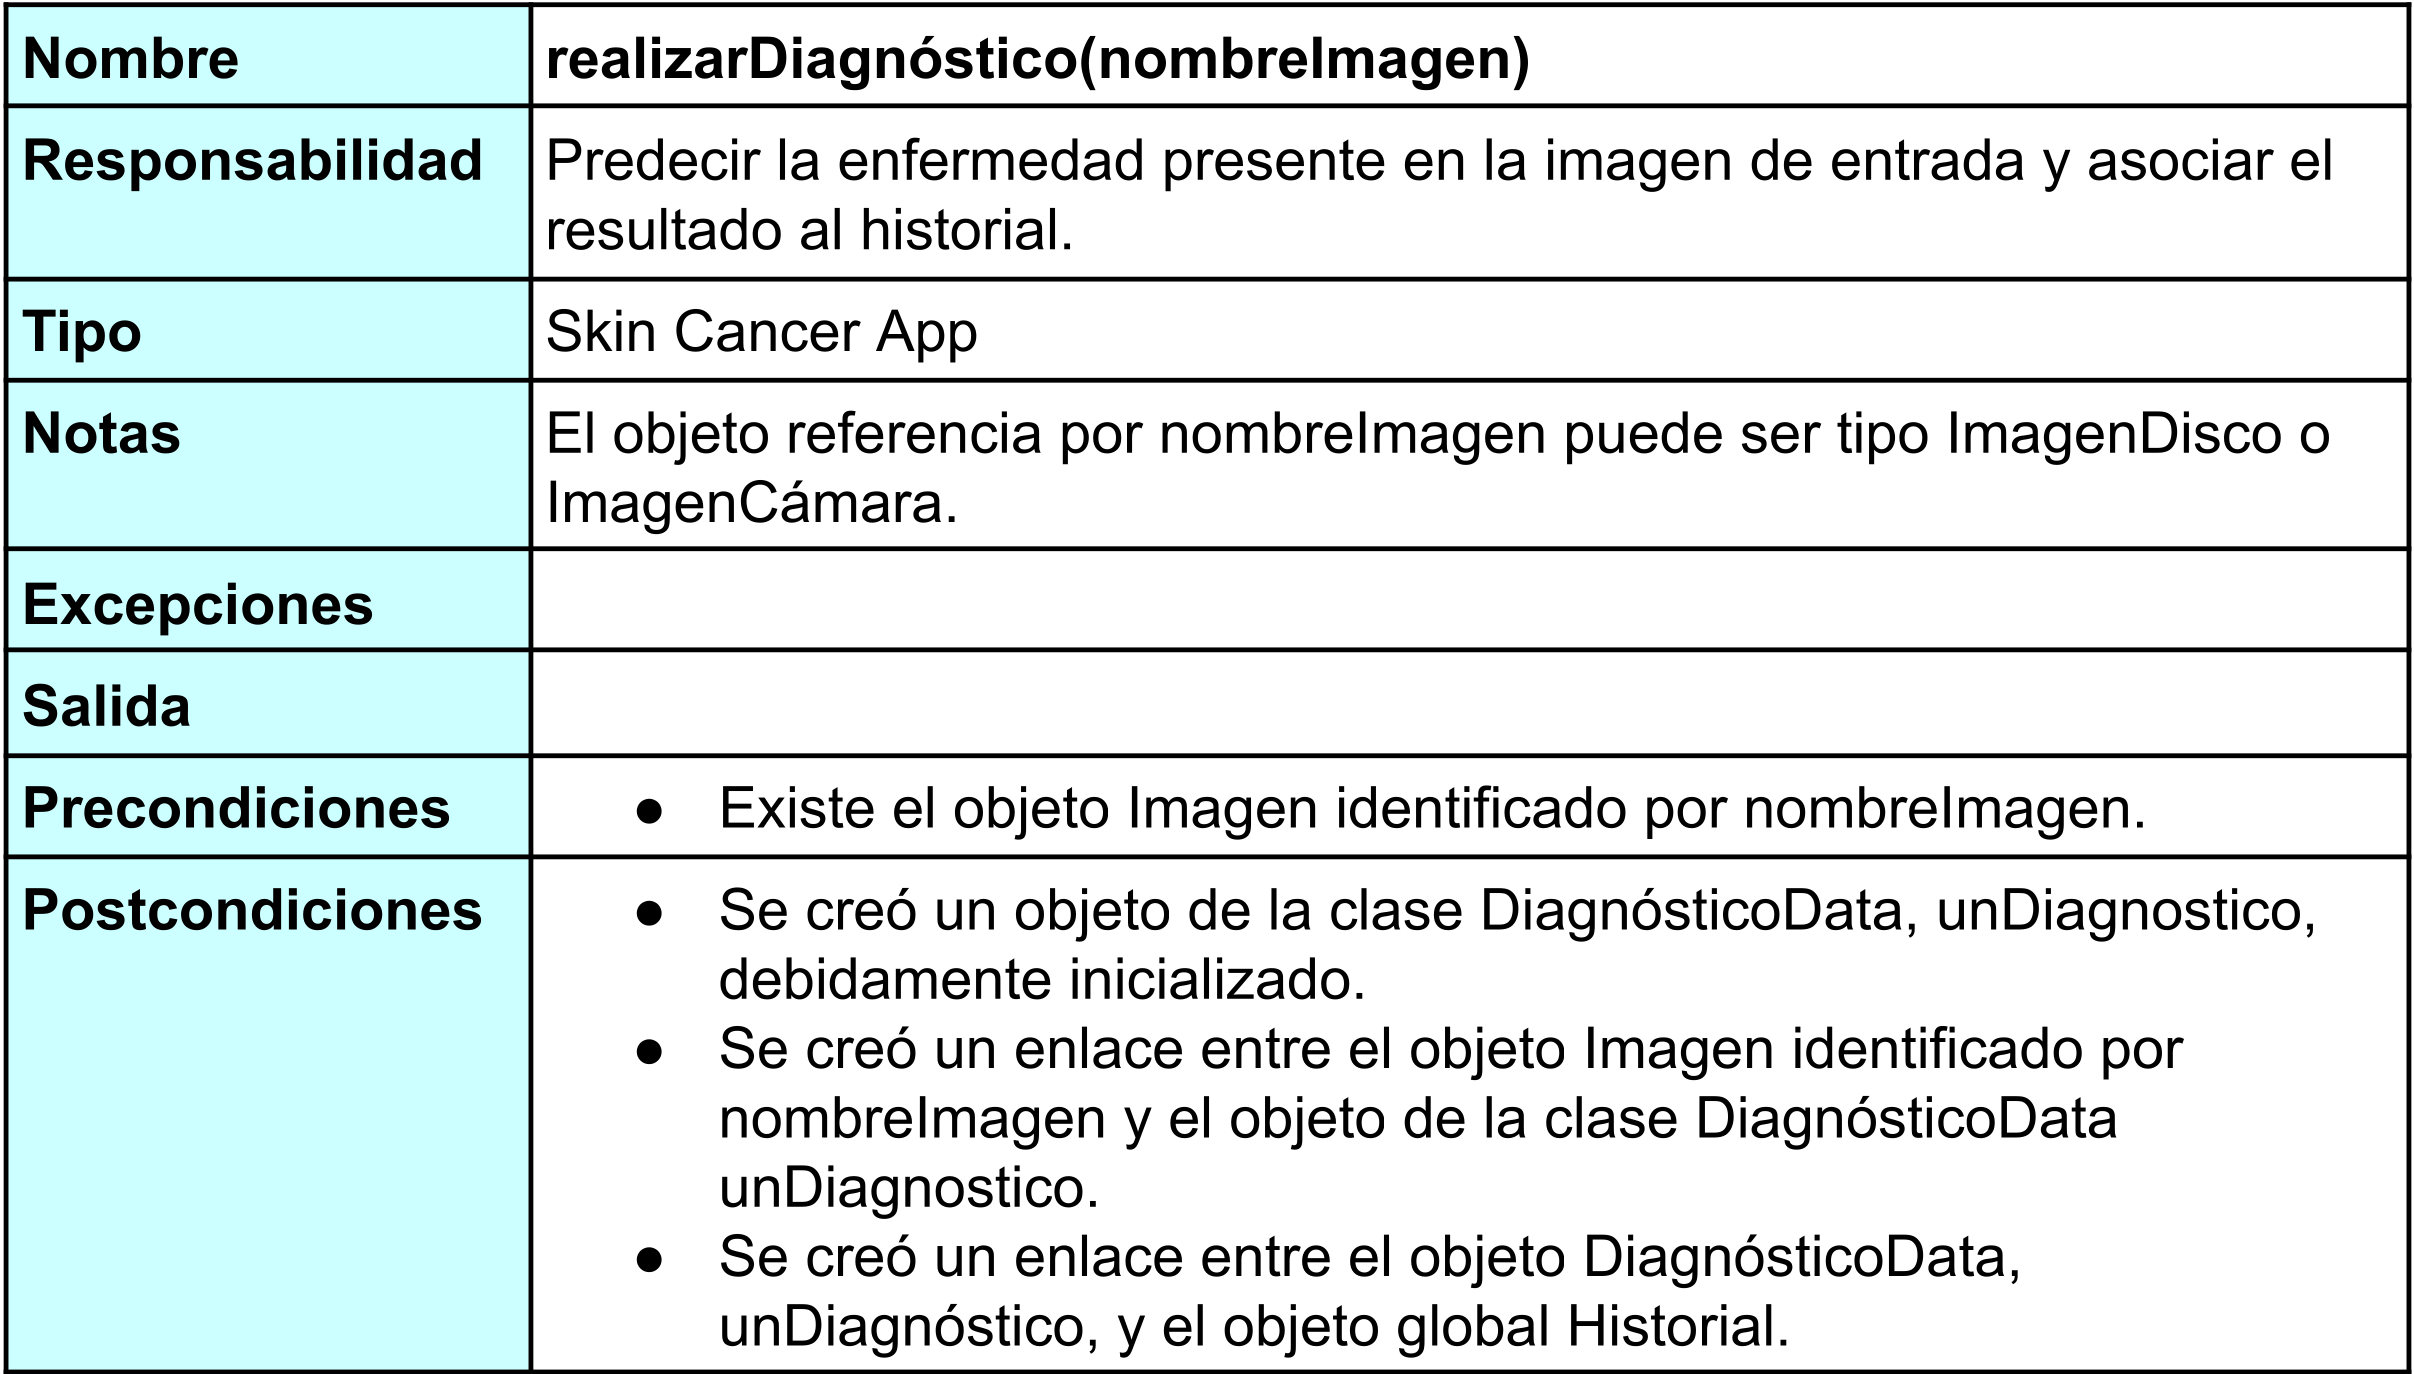
\includegraphics[scale = 0.16]{imagenes/contrato4.png}
 	\caption{Contrato: realizar diagnóstico.}
 	\label{fig:contrato4}
 \end{table}
 
   \begin{table}[H]
 	\centering
 	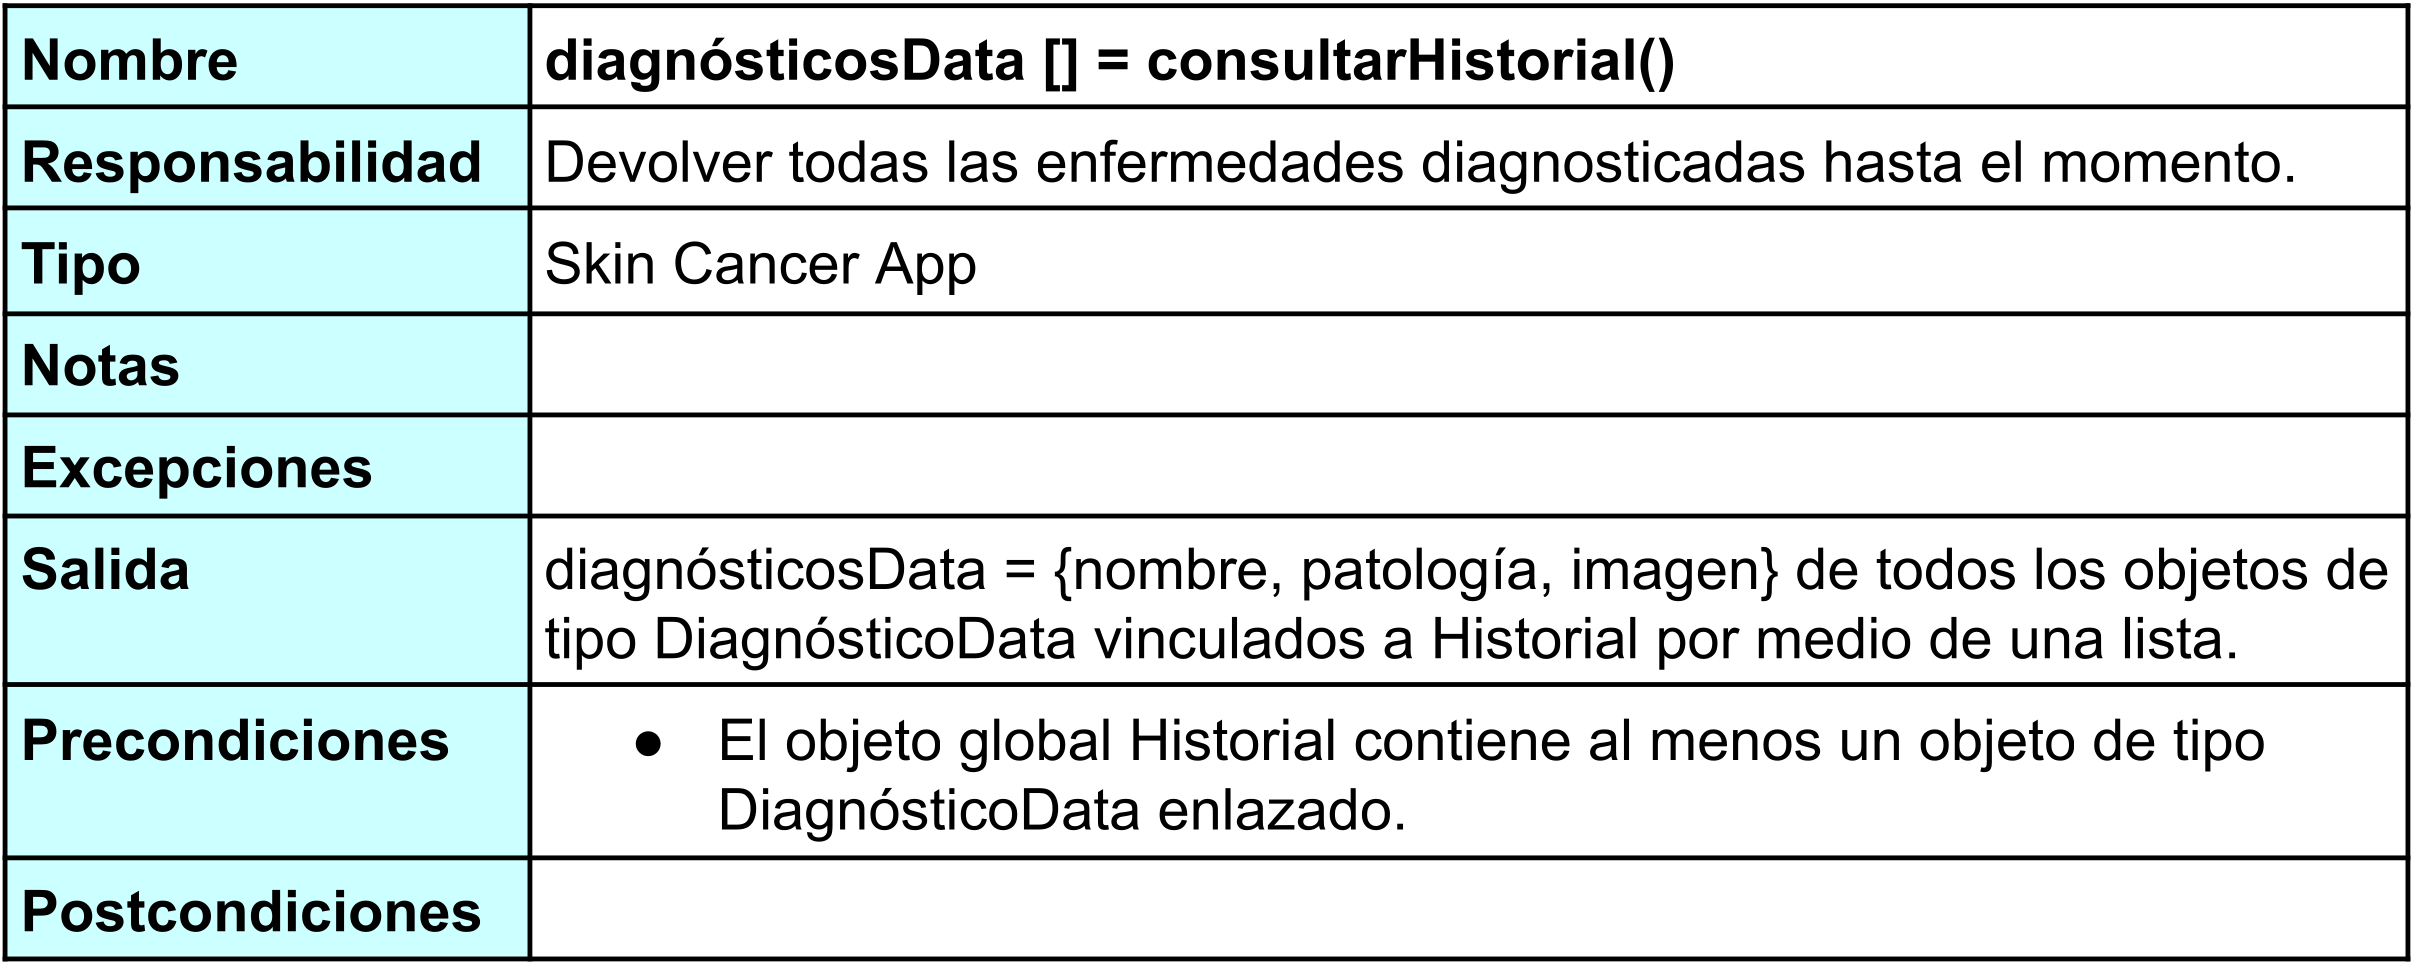
\includegraphics[scale = 0.16]{imagenes/contrato5.png}
 	\caption{Contrato: consultar historial.}
 	\label{fig:contrato5}
 \end{table}
 
    \begin{table}[H]
 	\centering
 	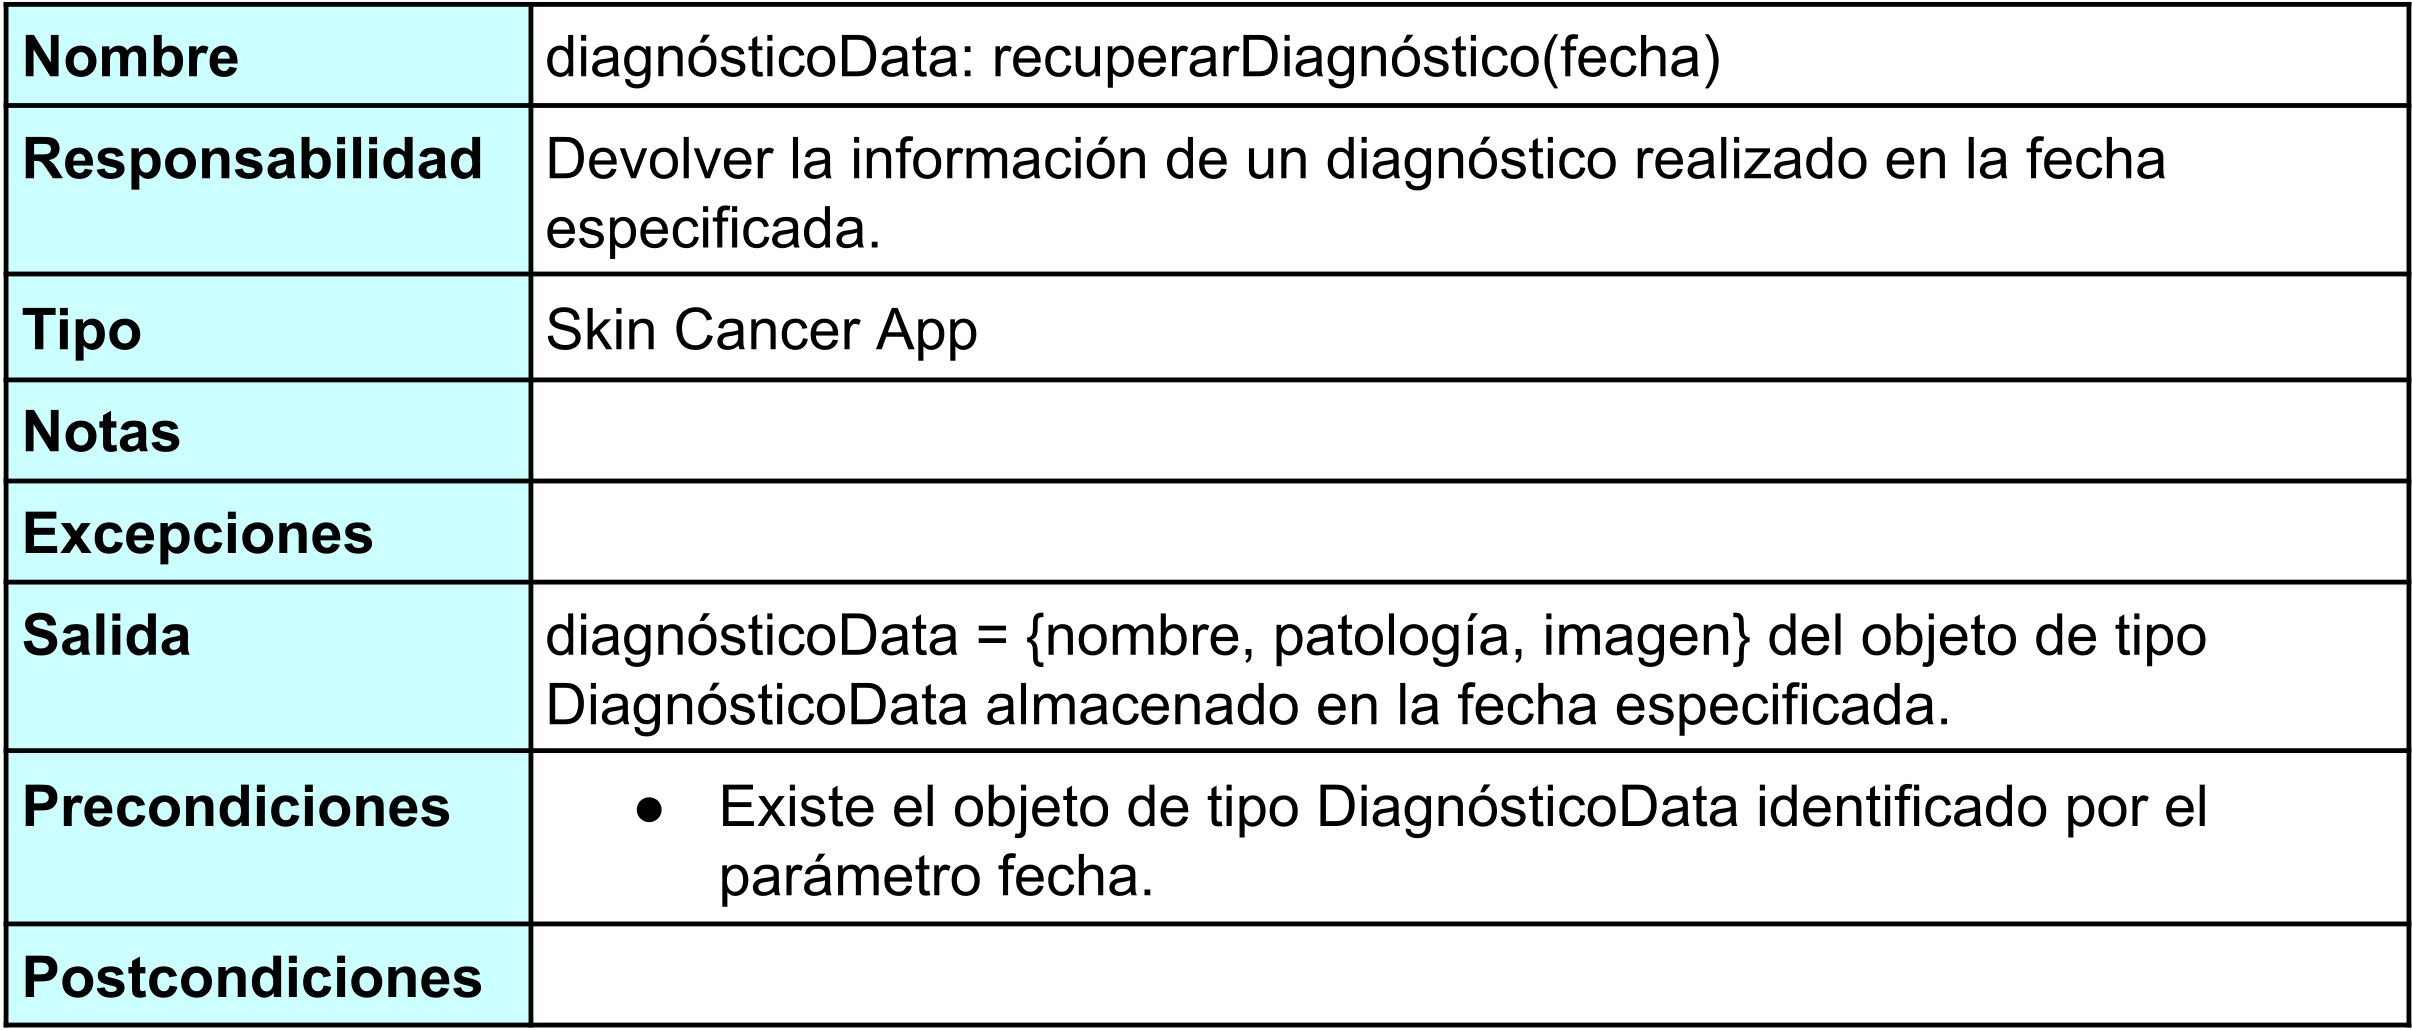
\includegraphics[scale = 0.315]{imagenes/contrato6.png}
 	\caption{Contrato: recuperar diagnóstico.}
 	\label{fig:contrato6}
 \end{table}
 
 Gracias a la definición formalizada en cada contrato, podemos trazar de forma específica los comportamientos de cada operación en diagramas de comunicación, para diseñar el modelo UML de clases de implementación, que describe la arquitectura definitiva del proyecto.
 
 \section{Diseño}
 
 La fase de diseño recoge la especificación final del sistema, teniendo como referencia los contratos y el diagrama conceptual asociado.
 
 En esta fase, llamada diseño por ser la fase previa a la implementación,  debemos crear los diagramas de comunicación (o interacción) de todas las
 operaciones especificadas en los contratos, y agregar posibles nuevas clases y atributos que no fueron especificados anteriormente, y que son requeridos para el correcto funcionamiento del sistema
 
 Toda esta información es recogida en el diagrama UML de clases del diseño, donde, partiendo del diagrama conceptual, se incluirán las clases con sus atributos y métodos, de los cuales se detallan la navegabilidad y la visibilidad de los atributos.
 
 \subsection{Diagramas de comunicación}
 
 Los diagramas de comunicación permiten observar con detalle el comportamiento interno de cada una de las operaciones del sistema. Si bien estas ya fueron especificadas en los contratos, el funcionamiento interno de la misma quedó en un segundo plano, ya que su objetivo era describir la operación sin entrar en detalles de implementación. Mediante los diagramas de comunicación presentes a continuación, podemos acercarnos un paso más al lenguaje del desarrollador. Siguiendo el orden de los contratos, podemos encontrar los diagramas  en ese mismo orden: tomar fotografía (\ref{fig:com1}),  seleccionar imagen (\ref{fig:com2}), recortar región de una imagen (\ref{fig:com3}), realizar diagnóstico (\ref{fig:com4}), consultar historial (\ref{fig:com5}) y recuperar diagnóstico (\ref{fig:com6}).
 
\begin{figure}[H]
 	\centering
 	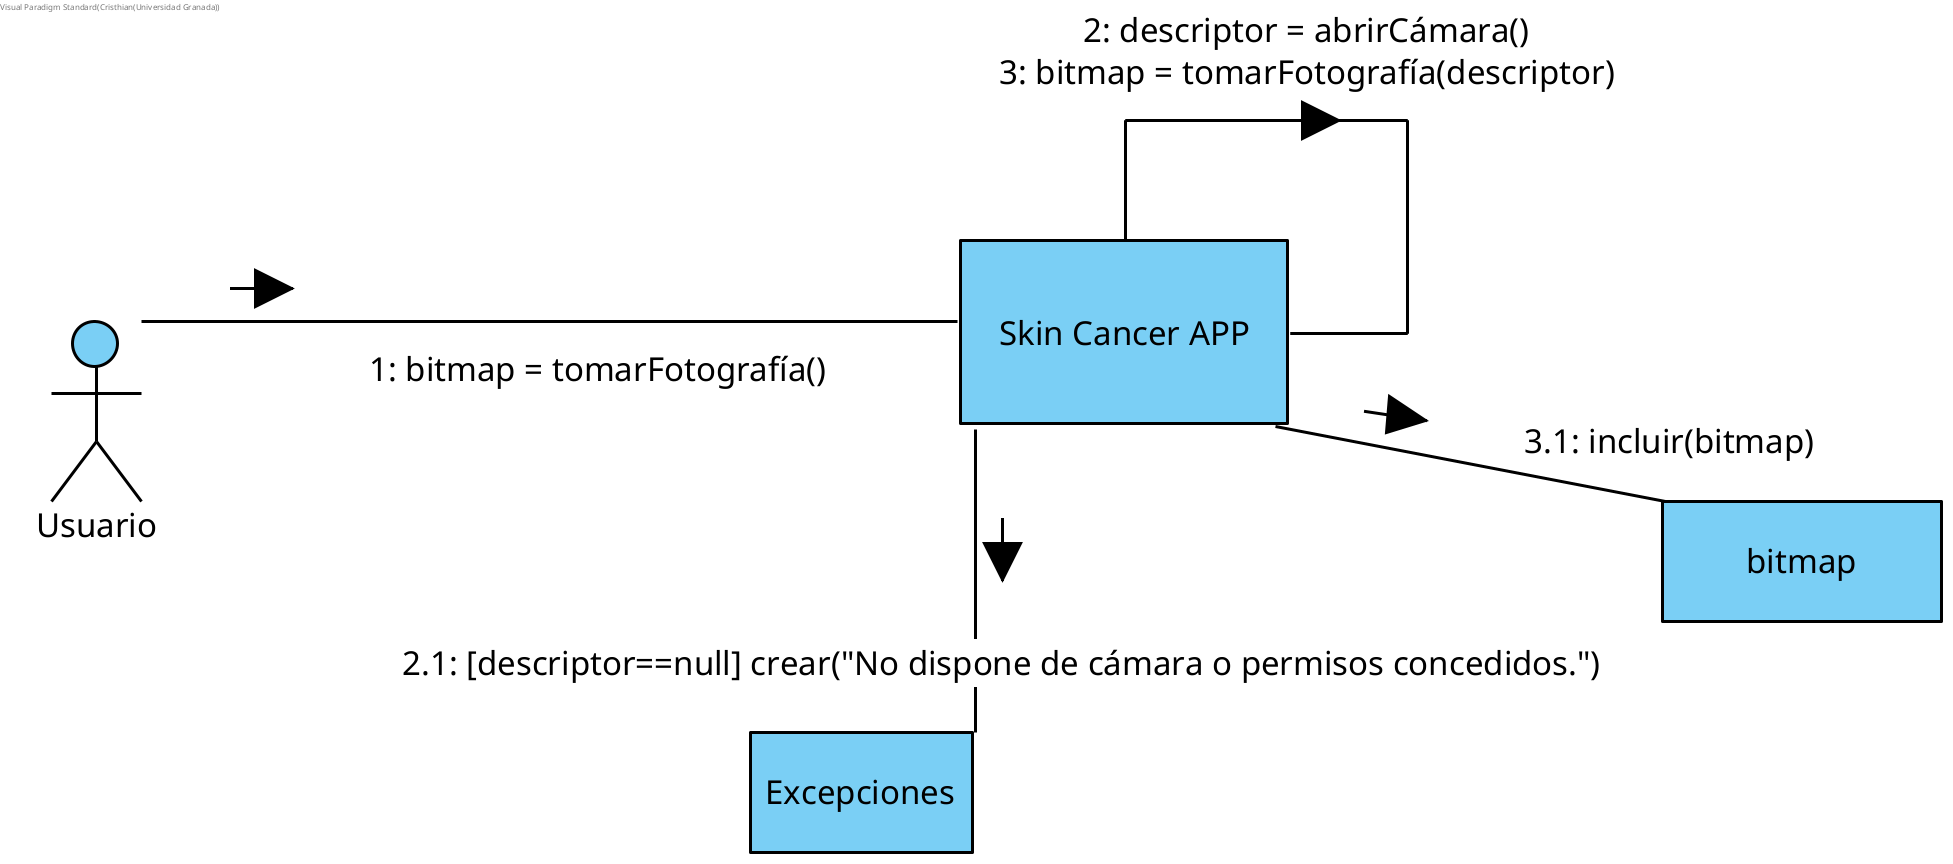
\includegraphics[scale = 0.8]{imagenes/TomarFotografía.png}
 	\caption{Diagrama de comunicación: tomar fotografía}
 	\label{fig:com1}
 \end{figure}
 
 
\begin{figure}[H]
 	\centering
 	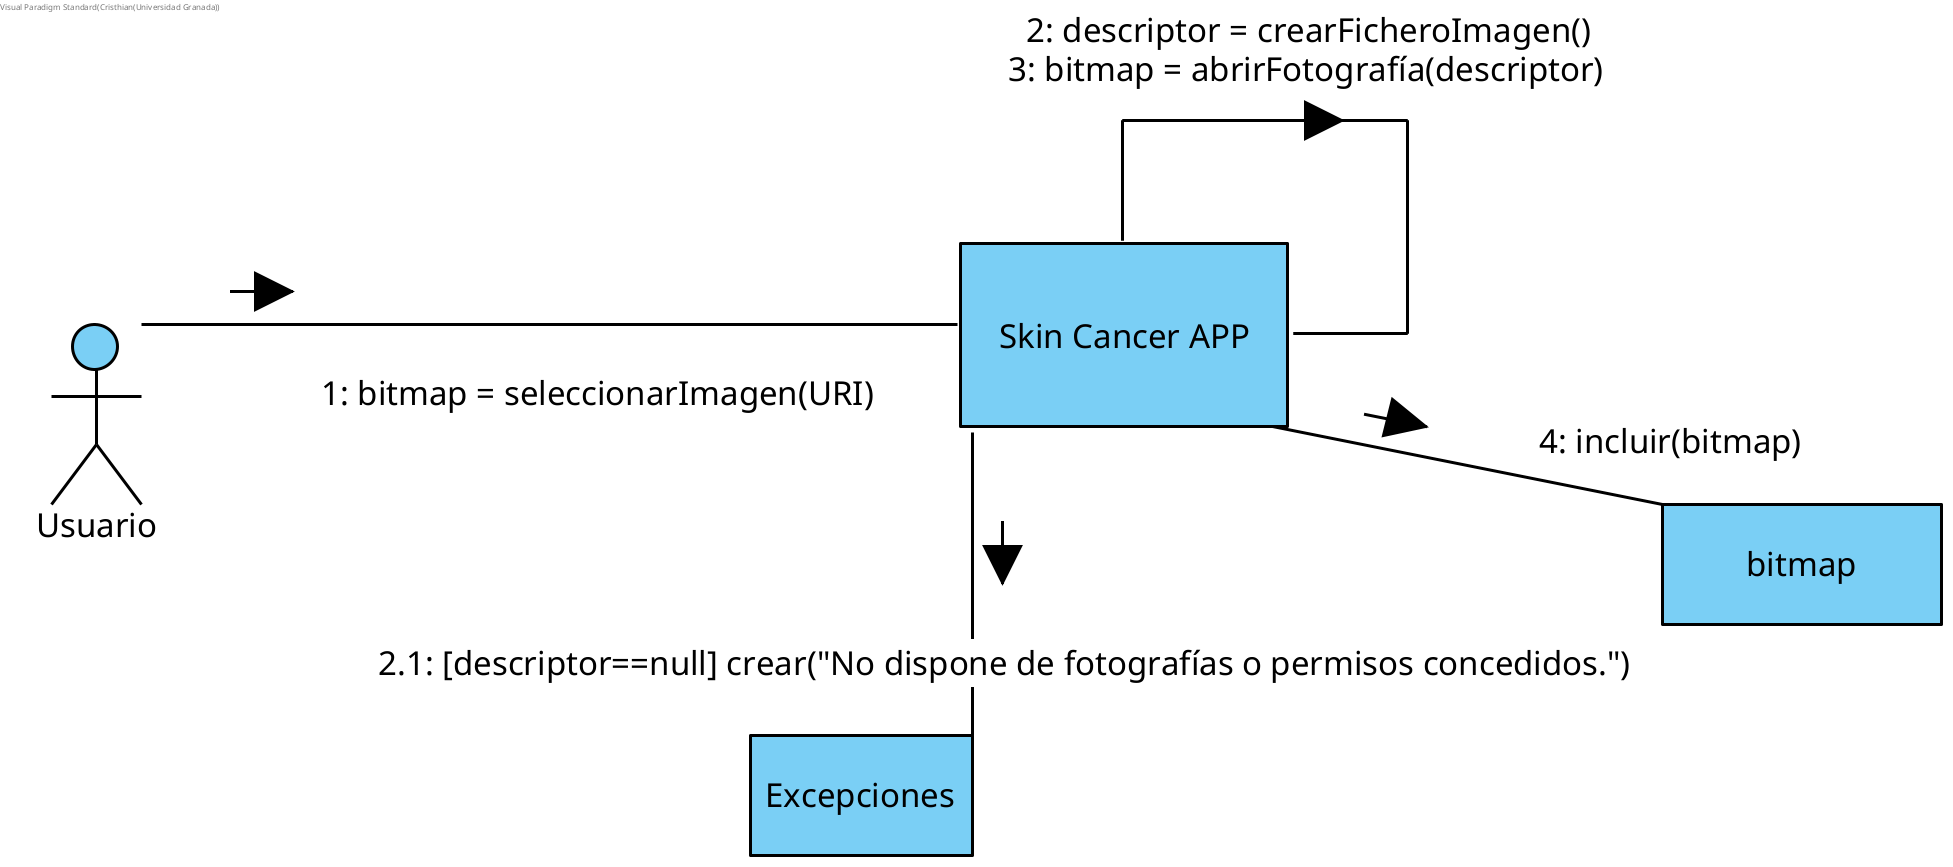
\includegraphics[scale = 0.8]{imagenes/SeleccionarImagen.png}
 	\caption{Diagrama de comunicación: seleccionar imagen}
 	\label{fig:com2}
 \end{figure}
 
\begin{figure}[H]
 	\centering
 	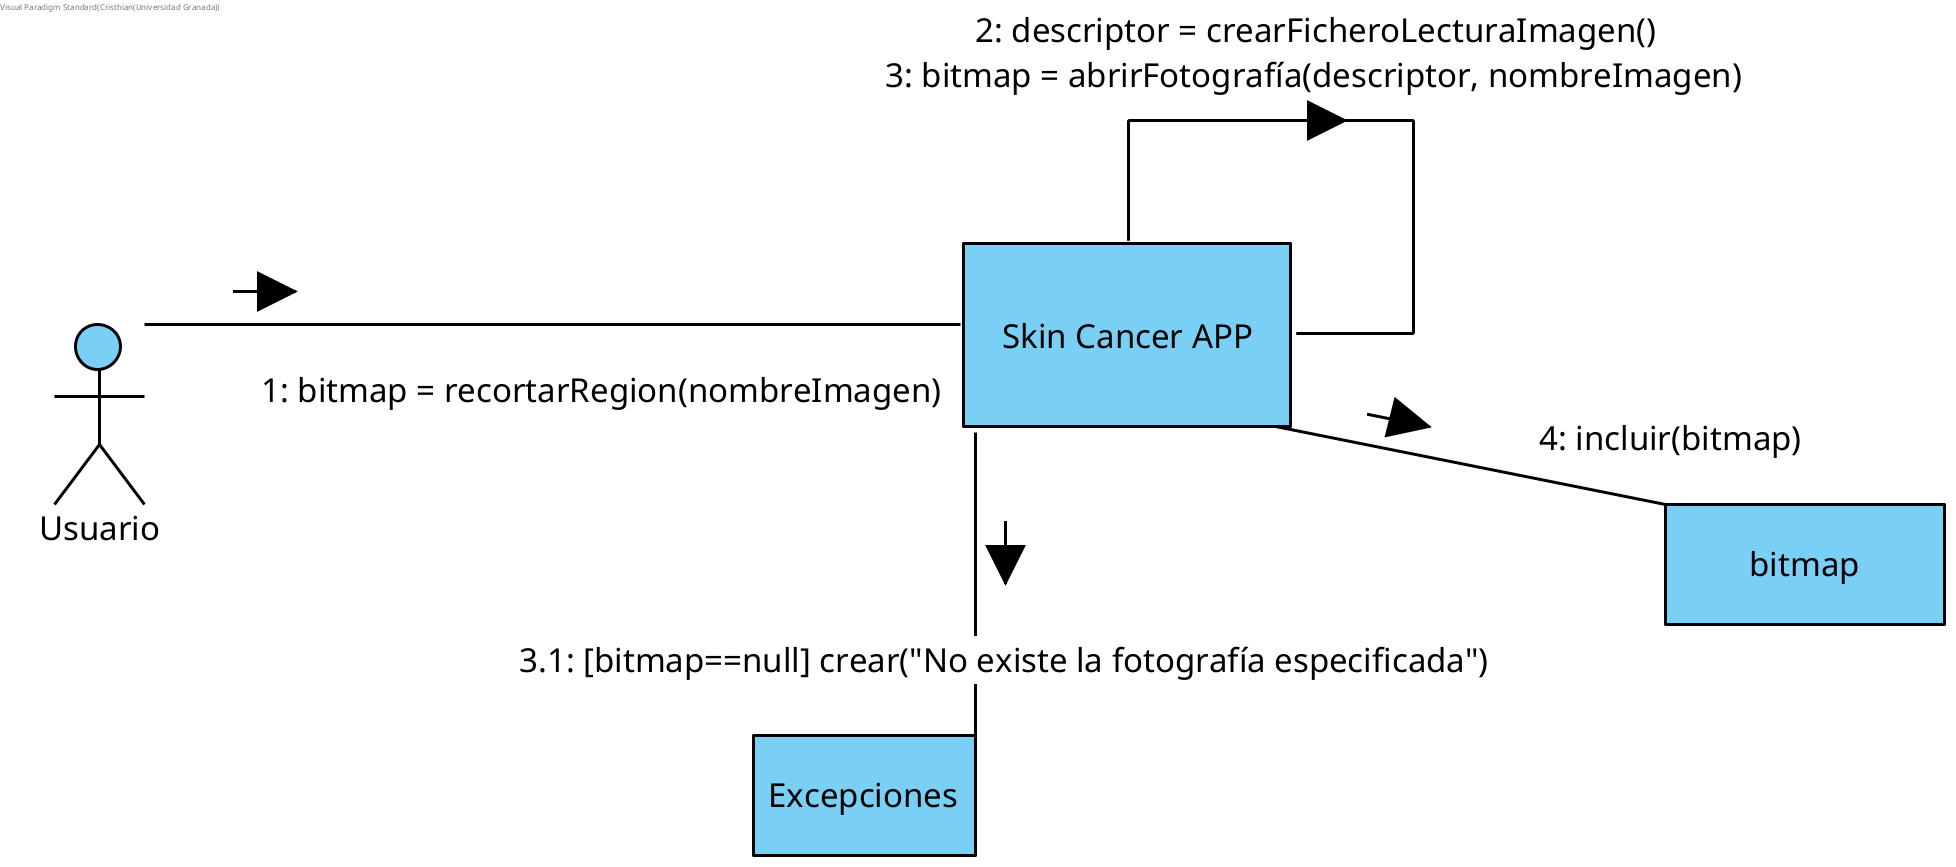
\includegraphics[scale = 0.8]{imagenes/RecortarRegión.png}
 	\caption{Diagrama de comunicación: recortar región}
 	\label{fig:com3}
 \end{figure}
 
 \begin{figure}[H]
 	\centering
 	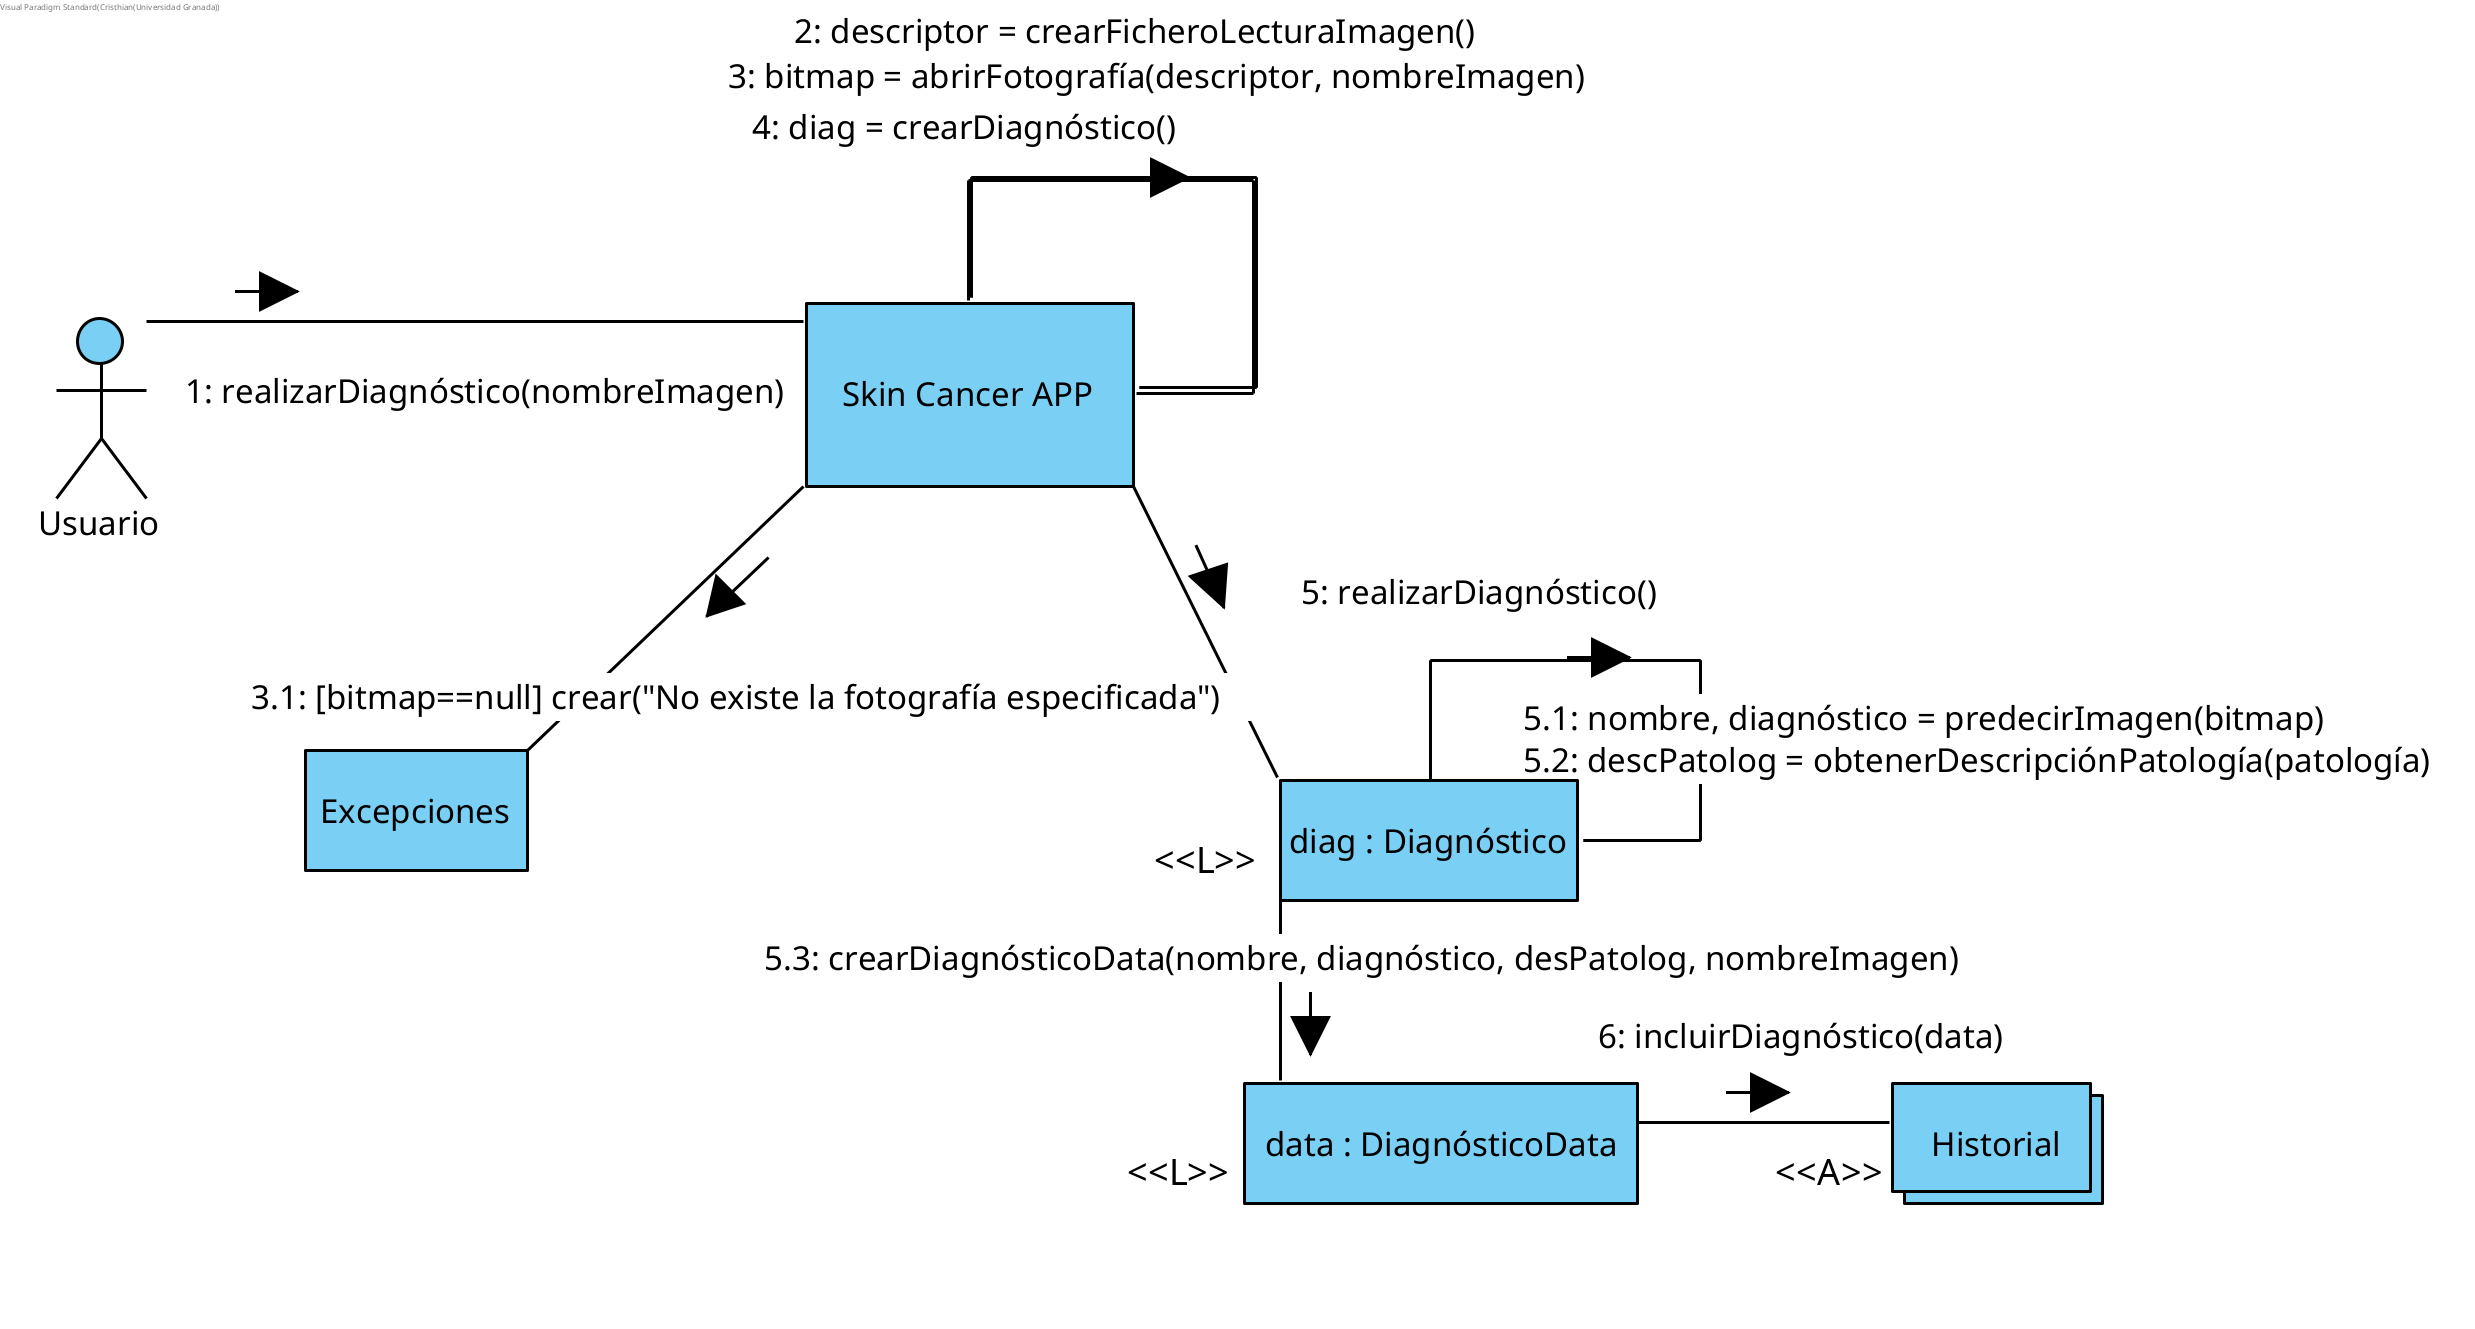
\includegraphics[scale = 0.75]{imagenes/RealizarDiagnóstico.png}
 	\caption{Diagrama de comunicación: realizar diagnóstico}
 	\label{fig:com4}
 \end{figure}
 
  \begin{figure}[H]
 	\centering
 	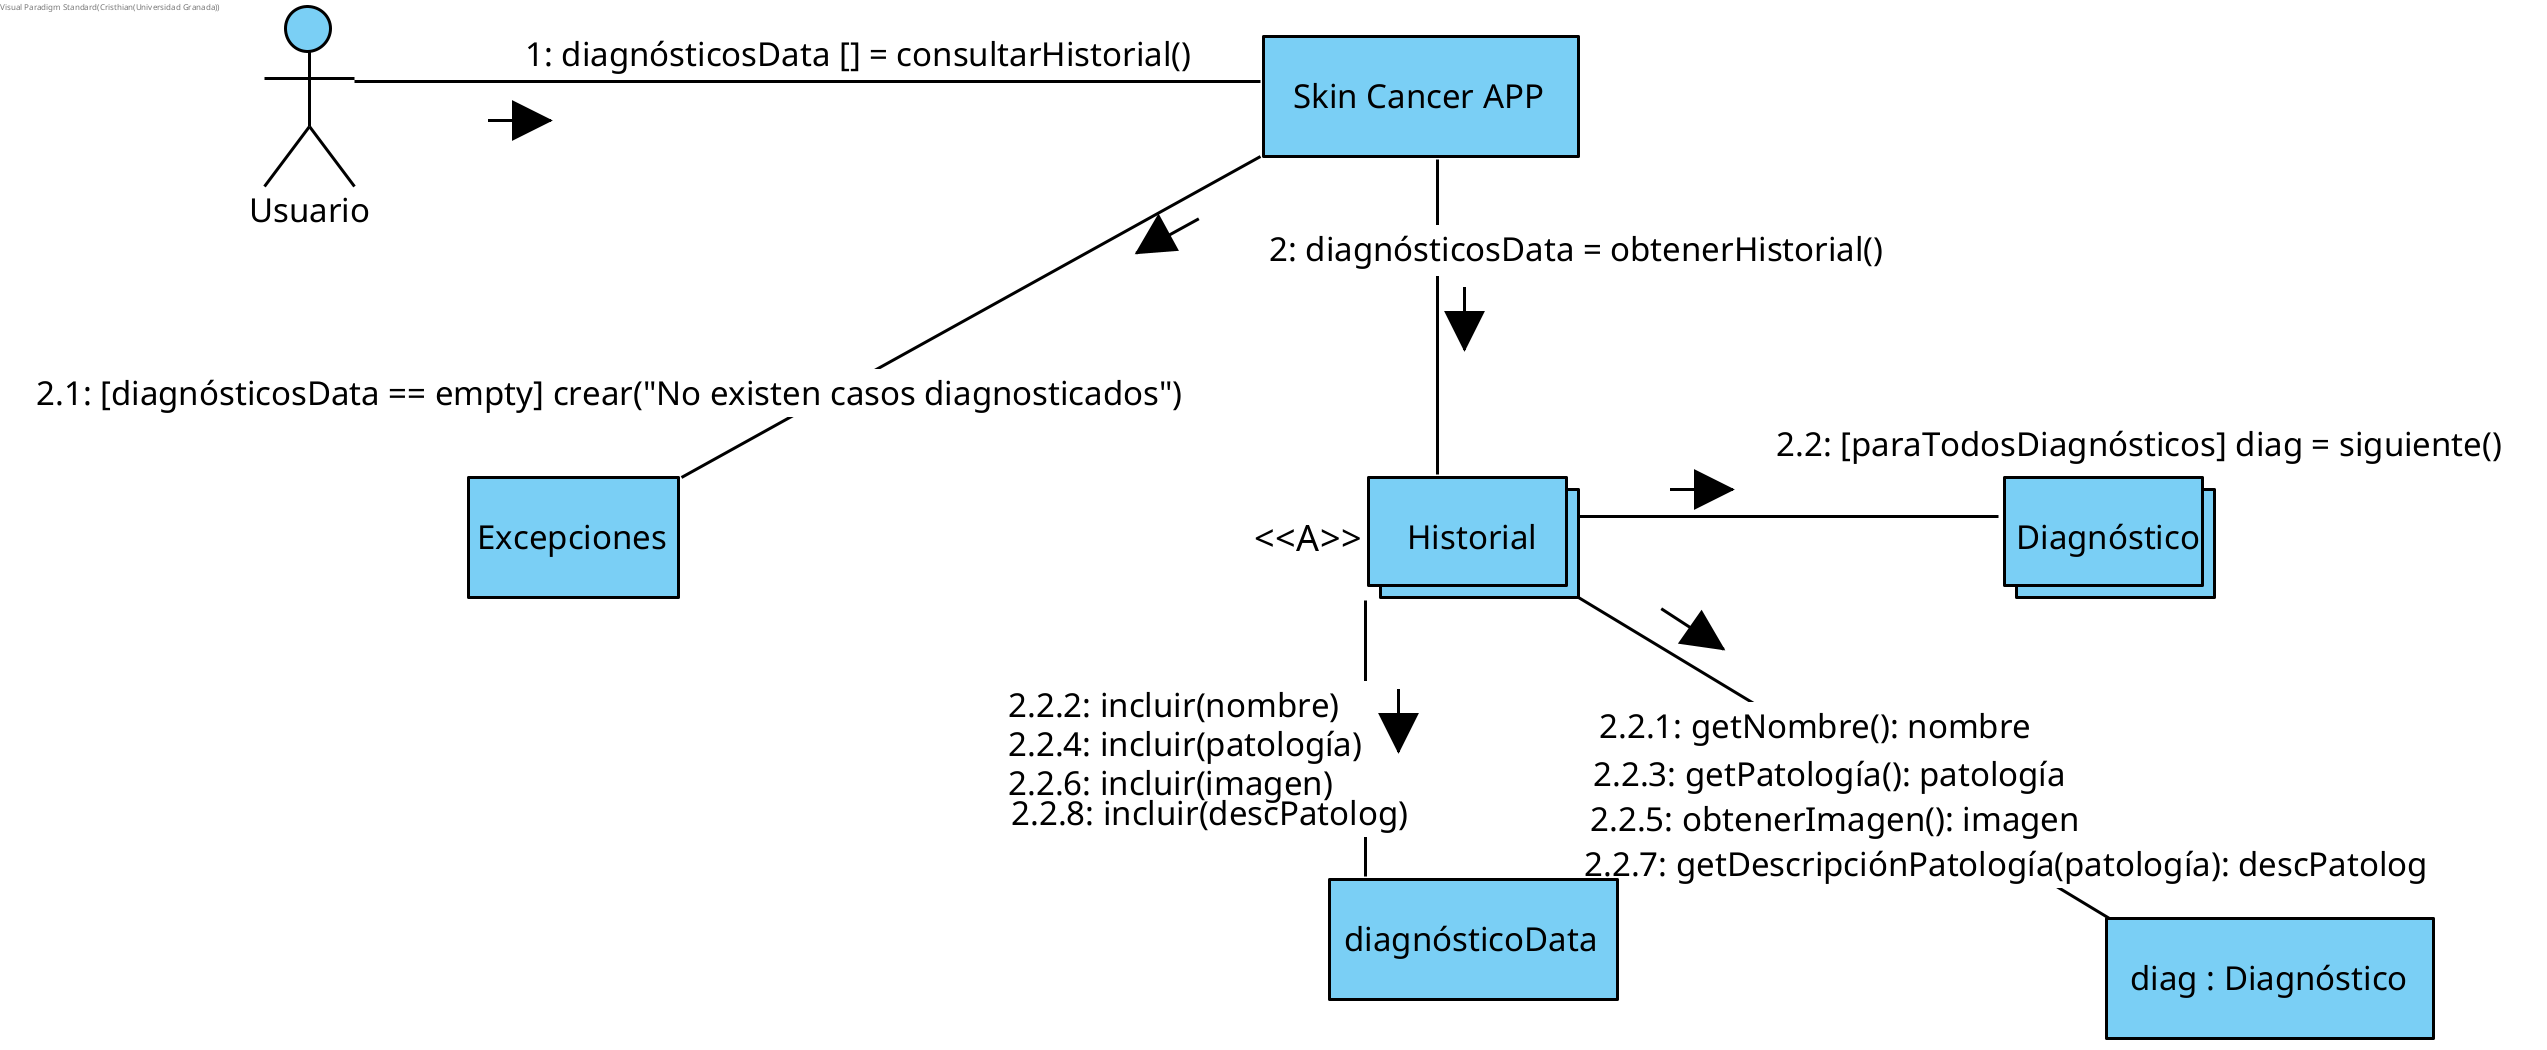
\includegraphics[scale = 0.75]{imagenes/HistorialSec.png}
 	\caption{Diagrama de comunicación: consultar historial}
 	\label{fig:com5}
 \end{figure}
 
 
   \begin{figure}[H]
 	\centering
 	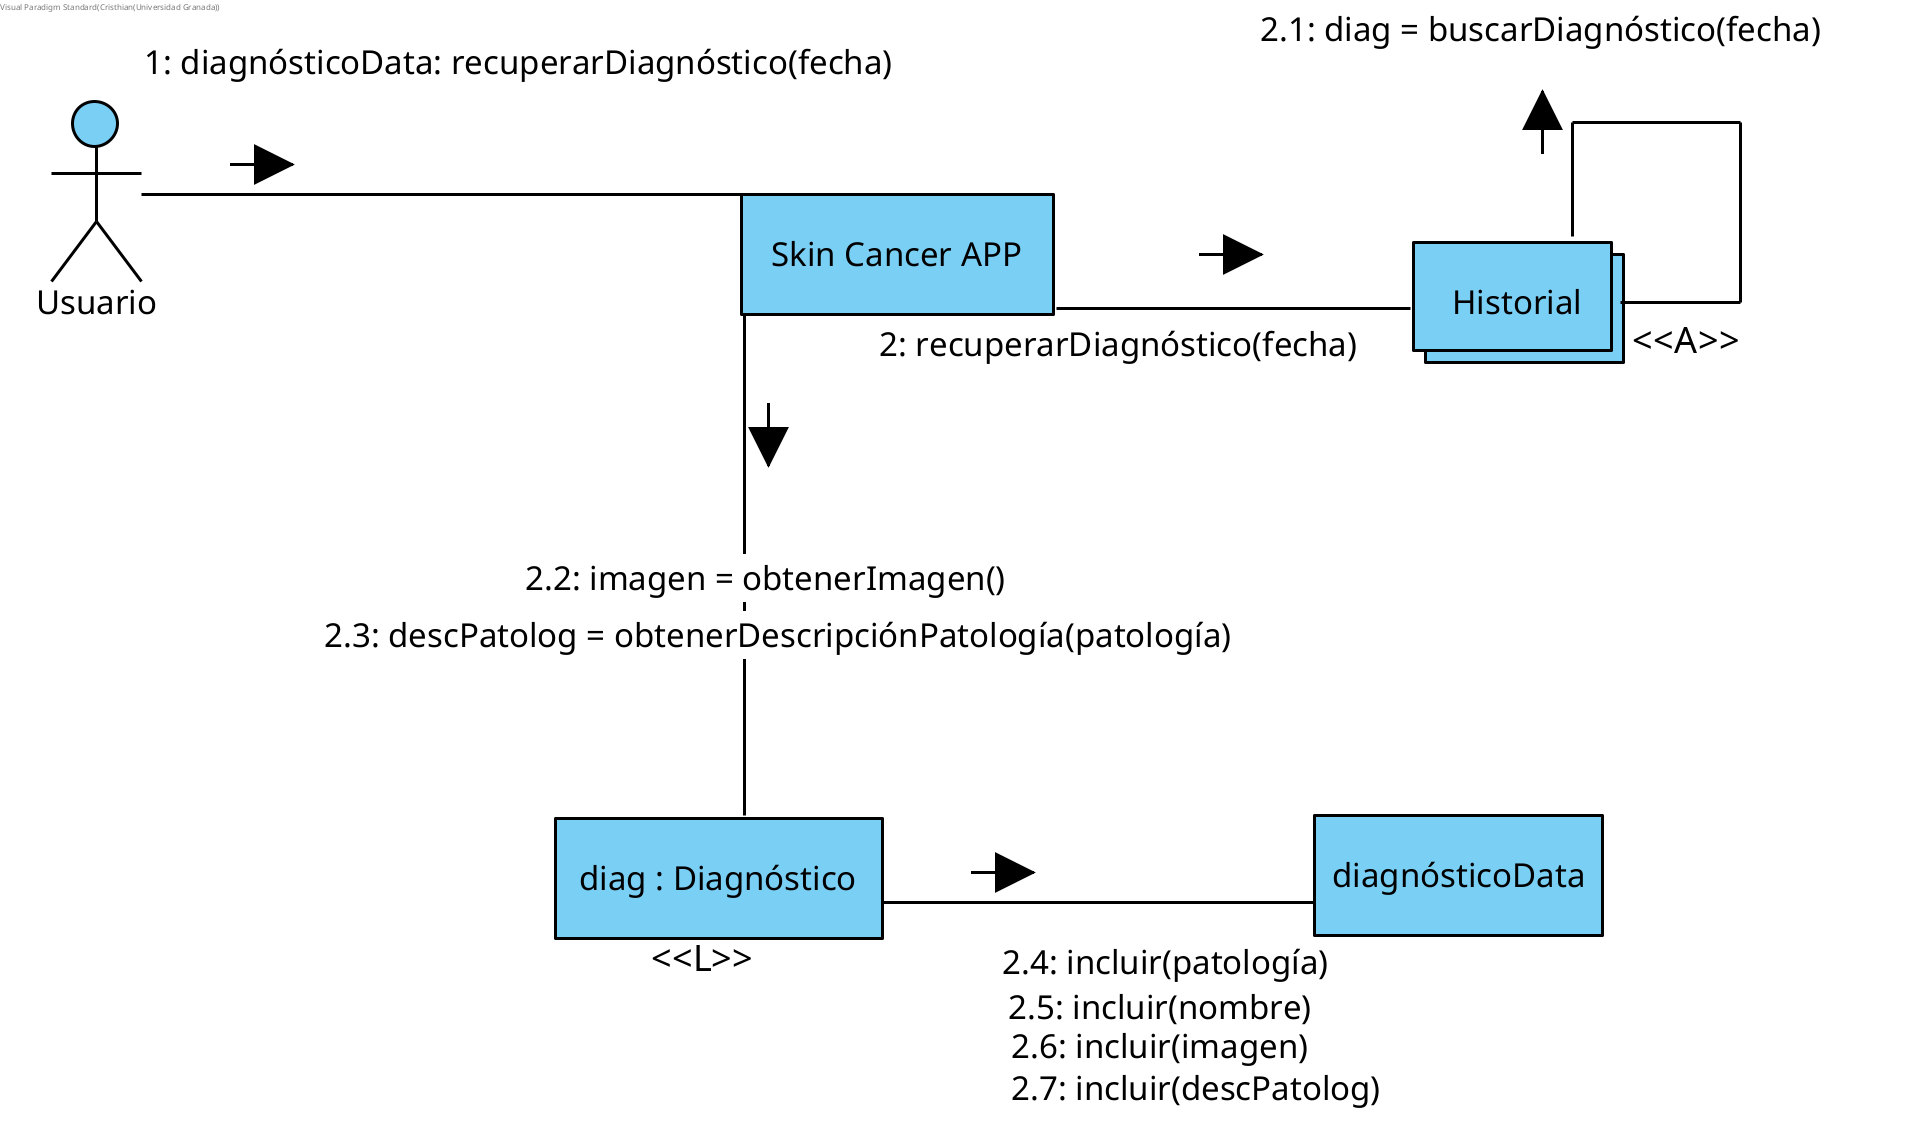
\includegraphics[scale = 0.75]{imagenes/GetDiagnóstico.png}
 	\caption{Diagrama de comunicación: consultar entrada de historial}
 	\label{fig:com6}
 \end{figure}
 
 Una vez establecido el comportamiento de forma específica, podemos pasar a la fase de creación del diagrama UML de clases.
 
 \subsection{Diagrama de clases de implementación}
 Este paso es el último antes de la implementación, por lo que debemos especificar adecuadamente cada una de las clases y métodos que realmente se requieren para crear la aplicación. La implementación se llevará a cabo empleando el IDE de Android Studio~\cite{androidstudio}, y siguiendo el patrón de implementación propuesto por Android.
  
 Su estructura es bastante diferente a la de un proyecto habitual; a pesar de emplear Java \cite{javalang} para la implementación de clases, la creación de una aplicación se centra en hacer uso de dos patrones principalmente: el uso de actividades y fragmentos, por lo que las clases presentes en el proyecto heredan de estas dos clases y producen cambios sustanciales en la estructura originalmente ideada. Si profundizamos en los conceptos de fragmento y actividad:
 
 \begin{itemize}
 	\item \textbf{Actividad}~\cite{actividad}. Unidad básica de ejecución de una aplicación Android, y permite mostrar el contenido de la aplicación. El ciclo de vida de una actividad comprende la creación de la misma, hasta su destrucción, cuando el sistema recupera los recursos de esa actividad. Es posible navegar entre actividades, realizando su declaración adecuadamente, aunque, como última tendencia, se suelen emplear fragmentos para realizar cambios de ventana.
 	\item \textbf{Fragmento}~\cite{fragmento}. Parte modular de la interfaz de usuario, la cual posee un ciclo vida con varias fases; principalmente, usaremos creación (método \textit{onCreate}), destrucción (\textit{onDestroy}) y actualización del contenido, mediante métodos implementados por nosotros mismos. Permite recoger las entradas y salidas del usuario, y normalmente, dependen de una actividad para funcionar.
 \end{itemize}
 
 Por tanto, al heredar de estas clases, deben incorporar los métodos de creación y destrucción, así como de actualización de información, y podemos obtener 3 subsistemas bien diferenciados: la pantalla de bienvenida de la aplicación, puramente informativa; el subsistema de diagnóstico y el subsistema de historial, siendo estos dos últimos los definidos en fases previas de esta tarea de diseño, pero que han requerido las modificaciones pertinentes para funcionar adecuadamente en el ecosistema Android.
 
 Podemos encontrar una visión general del sistema en el diagrama de la figura \ref{fig:clasesglobal}, así como una implementación del sistema de diagnóstico en la figura \ref{fig:clasesdiag} y el historial en la figura \ref{fig:claseshist}.
 
    \begin{figure}[H]
 	\centering
 	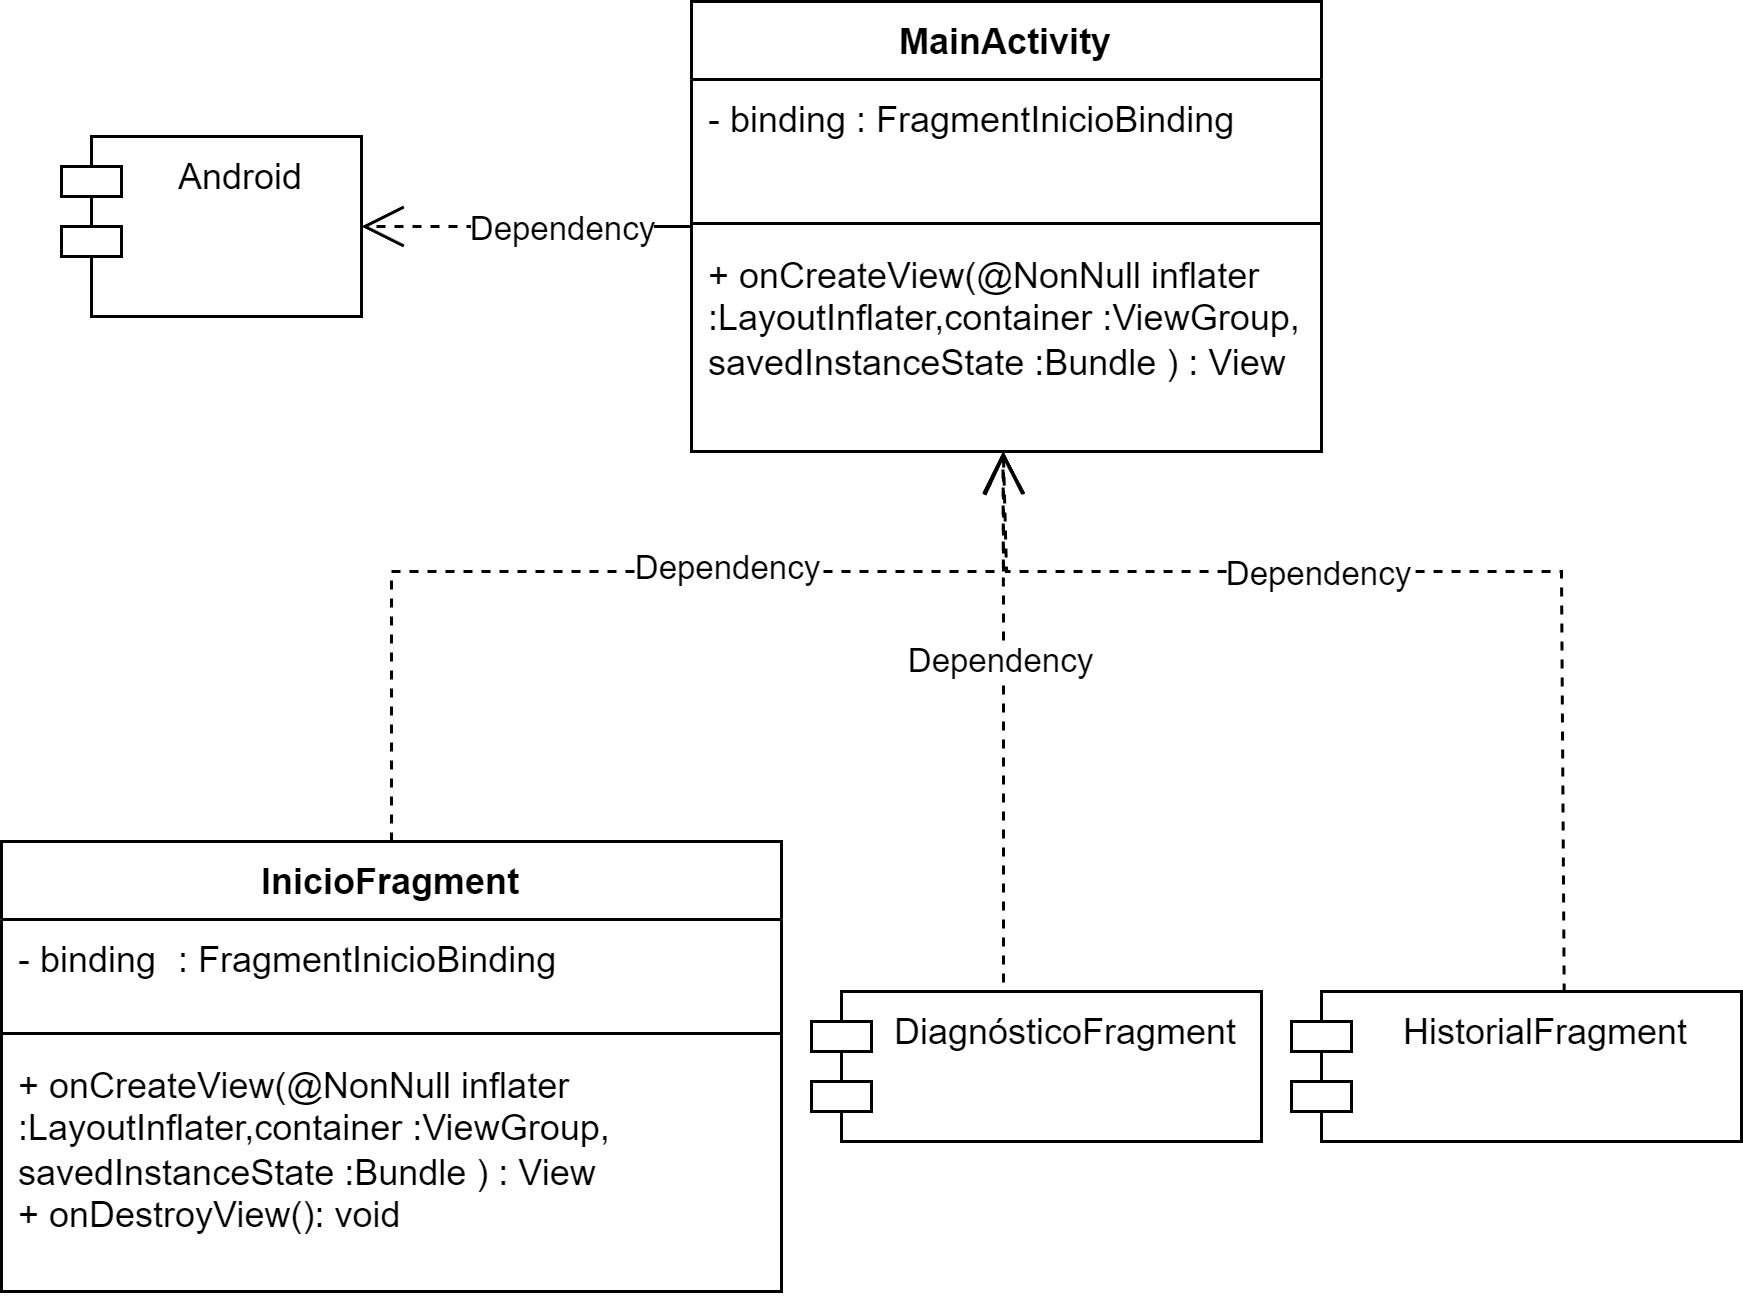
\includegraphics[scale = 0.75]{imagenes/DiagramaGeneral.png}
 	\caption{Diagrama de clases: visión general del sistema}
 	\label{fig:clasesglobal}
 \end{figure}
 
     \begin{figure}[H]
 	\centering
 	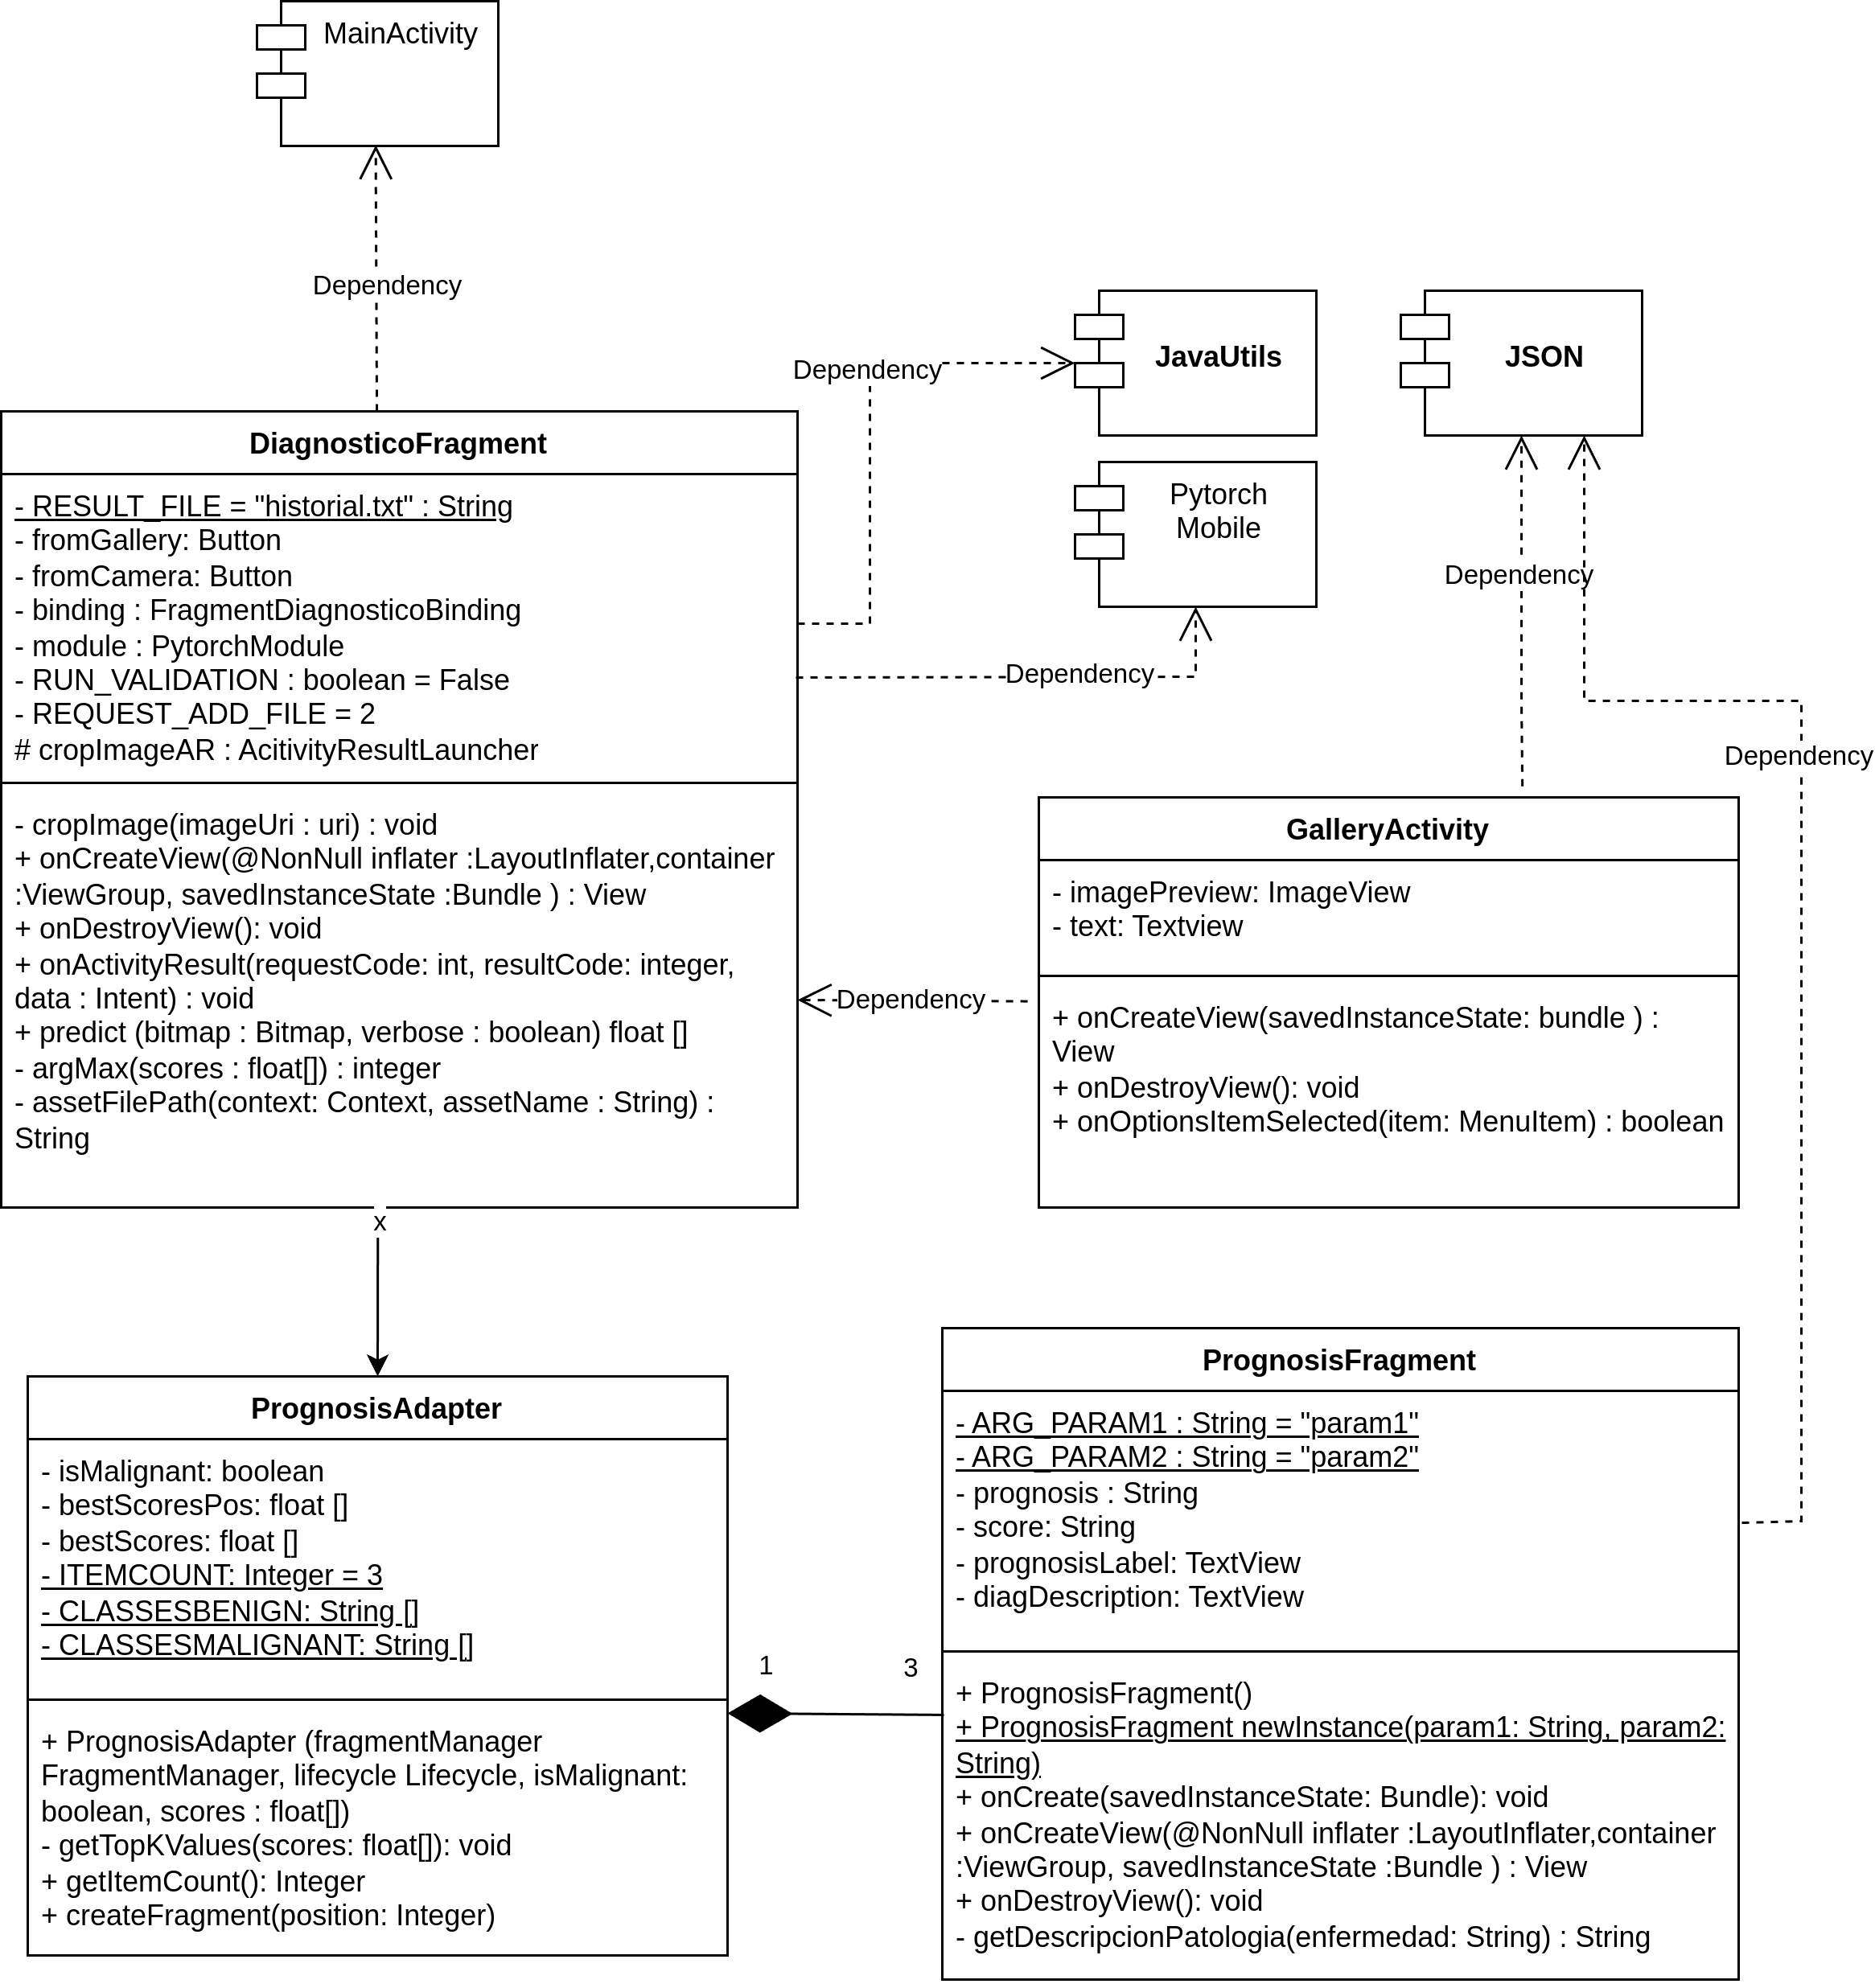
\includegraphics[scale = 0.75]{imagenes/androidAPP-Diagnostico.png}
 	\caption{Diagrama de clases: subsistema de diagnósticos}
 	\label{fig:clasesdiag}
 \end{figure}
 
      \begin{figure}[H]
 	\centering
 	\includegraphics[scale = 0.75]{imagenes/androidAPP-Historial.png}
 	\caption{Diagrama de clases: subsistema de historial}
 	\label{fig:claseshist}
 \end{figure}
 
 \section{Manual de uso de la aplicación}
 En este apartado, se muestra el comportamiento de la aplicación y todas las funcionalidades disponibles para facilitar al usuario su funcionamiento.  Aunque la aplicación muestra mensajes de retroalimentación y descripciones en la interfaz, destacaremos en este apartado de forma visual toda su disposición.
 
 Nada más proceder con su apertura, podemos encontrar 3 submenús distintos si hacemos uso del panel lateral de navegación (apreciable en la figura  \ref{fig:inicioapp}):
 \begin{itemize}
 	\item  \textbf{Pantalla de bienvenida}. Página principal al iniciar la aplicación. Muestra información previa acerca de la utilidad de la aplicación, consejos de cuidados para la piel, y una exención de responsabilidades, donde se informa del propósito plenamente informativo del producto (ver figura \ref{fig:inicioapp}).
 	\item \textbf{Sección de diagnóstico}. Menú que coincide con la descrita en los diagramas anteriores, en la cual el usuario puede especificar una imagen de galería o mediante la cámara para ser diagnosticada. Se explica con detalle en la sección \ref{sec:diag}.
 	\item \textbf{Sección de historial}. Menú en forma lista que muestra todos los casos diagnosticados por el paciente. Permite ver la imagen analizada, y la información del diagnóstico realizado. Profundizado en la sección \ref{sec:hist}.
 \end{itemize}
 
   \begin{figure}[H]
 	\centering
 	\subfigure[Pantalla de inicio]{\includegraphics[scale = 0.125]{imagenes/bievenidaapp.jpg}}
 	 \subfigure[Menú de navegación]{\includegraphics[scale = 0.125]{imagenes/menuapp.jpg}}
 	\caption{Interfaz de la aplicación: menús básicos}
 	\label{fig:inicioapp}
 \end{figure}
 
 \subsection{Realización de un diagnóstico}
  \label{sec:diag}
 La realización de un diagnóstico es la funcionalidad elemental de la aplicación. Es la actividad que contiene la mayor carga computacional  de la misma, ya que se requiere realizar la carga de modelos y se procede posteriormente a la inferencia del resultado.
 
 El proceso, descrito a modo guion, engloba los siguientes pasos:
 \begin{enumerate}
 	\item \textbf{Seleccionar la ventana de diagnóstico}. Haciendo uso del menú lateral, el usuario debe dirigirse a la segunda opción, llamada  \textbf{Diagnóstico}, y representada con el icono de una fotografía (figura \ref{fig:inicioapp}).
 	\item \textbf{Seleccionar método de importación}. Dentro de la actividad de diagnóstico, la aplicación nos permite realizar la importación de imagen a diagnosticar mediante dos medios: el uso de la galería, y la toma de una fotografía mediante la cámara. Para iniciar el proceso de importación, se debe pulsar uno de dos grandes botones azules en la parte inferior de la ventana, según el origen de la imagen (ver en figura \ref{fig:recortarapp}).
 	\begin{enumerate}
 		\item Si selecciona tomar fotografía, se solicitarán permisos de acceso a ella, y podrá tomar una fotografía con la aplicación de cámara por defecto de su dispositivo.
 		\item Si selecciona abrir galería, se mostrará una solicitud de acceso a memoria, y a continuación, se muestra la galería en modo mosaico para seleccionar la imagen que se desee, como se aprecia en la figura \ref{fig:recortarapp}.
 	\end{enumerate}
 	\item \textbf{Recortado}. Tras la importación de la fotografía mediante alguno de los medios, se ofrece de forma opcional realizar el recorte de la misma. Este mecanismo es útil si la cámara no es capaz de enfocar debido a la cercanía, o la imagen es demasiado grande. Su funcionamiento se basa en desplazar las esferas que marcan las esquinas de la imagen para modificar el tamaño, y arrastrando desde el centro del rectángulo en caso de que se desee desplazar la región, como se puede apreciar en la figura \ref{fig:recortarapp}.
 	
 	\item \textbf {Comunicación del resultado}. Tras el recorte, se procede a realizar la clasificación de la imagen y a mostrar los resultados del diagnóstico de forma el usuario pueda comprender qué enfermedad sufre. Se muestran los campos enunciados a continuación y en la figura \ref{fig:diagnostico}.
 	\begin{itemize}
 		\item \textit{Bondad del resultado}. Especifica si se trata de una imagen benigna o maligna, y el porcentaje de seguridad del modelo. No representa una opinión médica real, sólo un valor indicativo procedente del modelo subyacente.
 		\item \textit{Tipo de enfermedad}. Tras la predicción binaria, se ha realizado también en segundo plano la clasificación mediante los modelos especializados, de forma que se muestran las tres enfermedades con mayor porcentaje de coincidencias dentro del conjunto benigno o maligno.
 		\item \textit{Descripción}. A título informativo, se muestra en pantalla una breve descripción acerca de la gravedad de la enfermedad, posibles orígenes y formas que posee.
 	\end{itemize}
 	
 	El usuario dispone de la posibilidad de desplazar hacia la izquierda el recuadro de la descripción para observar otras dos posibles clases que con un valor de probabilidad especificado pudieran tratarse de posibles alternativas (figura \ref{fig:diagnostico}).
 \end{enumerate}
 
    \begin{figure}[!ht]
 	\centering
 	\subfigure[Importación desde galería]{\includegraphics[scale = 0.125]{imagenes/galeriaapp.jpg}}
 	\subfigure[Recorte de la sección]{\includegraphics[scale = 0.125]{imagenes/recorteapp.jpg}}
 	\caption{Interfaz de la aplicación: selección desde galería y recorte de imágenes}
 	\label{fig:recortarapp}
 \end{figure}
 
     \begin{figure}[!ht]
 	\centering
 	\subfigure[Diagnóstico benigno (mediante cámara)]{\includegraphics[scale = 0.125]{imagenes/diagnosticobenigno.jpg}}
 	\subfigure[Diagnóstico maligno (mediante galería)]{\includegraphics[scale = 0.125]{imagenes/diagnosticoapp.jpg}}
 	\caption{Interfaz de la aplicación: selección desde galería y recorte de imágenes}
 	\label{fig:diagnostico}
 \end{figure}
 
 
 \subsection{Consulta del historial}
 \label{sec:hist}
 
 Todos los diagnósticos realizados por el usuario son almacenados en un fichero JSON, el cual simula el comportamiento de una base de datos local. Son almacenadas en formato lista, de forma que si requiere comprobar la evolución de la enfermedad, sea capaz de comparar las imágenes y observar el diagnóstico ofrecido en aquel momento.  Para acceder a él, simplemente se deben seguir los pasos a continuación:
 
 \begin{enumerate}
 	\item \textbf{Seleccionar ventana de diagnóstico}. De la misma forma que la iniciación de la acción de diagnóstico, debemos seleccionar en el panel lateral el botón \textbf{Historial}, representado con un icono de elementos apilados.
 	\item \textbf{Búsqueda del diagnóstico}. Una vez accedido, es posible buscar el diagnóstico de interés gracias a su ordenado de mayor a menor cronología; es decir, los casos más antiguos aparecen primero, y los más recientes, últimos. La información proporcionada engloba:
 	\begin{enumerate}
 		\item \textit{Tipo de enfermedad}. Si el caso es maligno o benigno.
 		\item \textit{Diagnóstico}. Enfermedad específica con mayor valor de probabilidad.
 		\item \textit{Imagen}. Se crea la miniatura de la imagen durante el diagnóstico para ser mostrada en esta sección e identificar más fácilmente el caso a buscar. Adicionalmente, en caso de necesidad de comprobar la imagen completa, se guarda una copia de cada recorte realizado en la galería del dispositivo. Estas podrían ser borradas, pero la miniatura permanecería en el historial.
 	\end{enumerate}
 \end{enumerate}
 
 En la figura \ref{fig:historial}, podemos observar un ejemplo de la distribución de los casos, los cuales se almacenan en formato de lista deslizable mediante scroll.
 
      \begin{figure}[H]
 	\centering
 	\includegraphics[scale = 0.125]{imagenes/historialapp.jpg}
 	\caption{Interfaz de la aplicación: historial}
 	\label{fig:historial}
 \end{figure}
	
	\input{capitulos/08_Implementación}
	
	%\chapter{Pruebas de uso}

	
	%\chapter{Conclusiones y trabajos futuros}

	
	
	%\chapter{Conclusiones y Trabajos Futuros}
	%
	%
	\nocite{}
	\bibliography{bibliografia/bibliografia}
	\bibliographystyle{plain}
	
	\appendix
	%\input{apendices/manual_usuario/manual_usuario}
	%\input{apendices/paper/paper}
	%%\input{glosario/entradas_glosario}
	% \addcontentsline{toc}{chapter}{Glosario}
%	 \printglossary
	%\chapter*{}
	\thispagestyle{empty}

\end{document}
